\documentclass[11pt,oneside]{book}
\usepackage[a4paper,margin=1in]{geometry}
\usepackage[T1]{fontenc}
\usepackage[utf8]{inputenc}
\usepackage{lmodern}
\usepackage{microtype}
\usepackage{amsmath,amssymb,amsthm,mathtools}
\usepackage{booktabs,longtable,array}
\usepackage{xcolor}
\usepackage{enumitem}
\usepackage{hyperref}
\usepackage{fancyhdr}
\usepackage{makeidx}
\usepackage{url}
\usepackage{cite}
\usepackage{graphicx}

\definecolor{deepblue}{RGB}{20,55,110}
\hypersetup{colorlinks=true,linkcolor=deepblue,citecolor=deepblue,urlcolor=deepblue,pdftitle={The Abacus Medal: Human Ideas in Mathematical Information Sciences},pdfauthor={}}
\pagestyle{fancy}
\fancyhf{}
\fancyhead[L]{\nouppercase{\leftmark}}
\fancyhead[R]{\thepage}
\setlength{\headheight}{14pt}
\setcounter{tocdepth}{0}
\makeindex

\newtheorem{definition}{Definition}[chapter]
\newtheorem{theorem}[definition]{Theorem}
\newtheorem{proposition}[definition]{Proposition}
\newtheorem{remark}[definition]{Remark}
\newcommand{\E}{\mathbb{E}}
\newcommand{\R}{\mathbb{R}}
\newcommand{\PP}{\mathbb{P}}
\newcommand{\eps}{\varepsilon}
\newcommand{\norm}[1]{\left\lVert #1\right\rVert}
\newcommand{\abs}[1]{\left\lvert #1\right\rvert}
\newcommand{\booknote}[1]{\begin{quote}\small\textit{#1}\end{quote}}
\newcommand{\expandedchapterspacing}{\renewcommand{\baselinestretch}{1.35}\selectfont}
\newcommand{\longchapterspacing}{\renewcommand{\baselinestretch}{1.8}\selectfont}
\newcommand{\targetchapterspacing}{\renewcommand{\baselinestretch}{2.5}\selectfont}
\newcommand{\normalchapterspacing}{\renewcommand{\baselinestretch}{1}\selectfont}
\newcommand{\hint}[1]{\newline\small\textit{Hint: #1}}

\title{The Abacus Medal\\[0.4em]\large Human Intuition and Mathematical Exploration in Information Sciences}
\author{}
\date{2026}

\begin{document}
\frontmatter
\maketitle
\chapter*{How to Read This Book}
The IMU Abacus Medal recognizes outstanding contributions to the mathematical aspects of information sciences. This book is not a catalogue of medals, affiliations, or publication lists. It is a set of invitations to think: what question was hiding inside a technical obstacle, what representation made the obstacle visible, and how can a student learn to search for the next representation?

The official IMU list names Shayan Oveis Gharan as the 2026 recipient and Mark Braverman as the 2022 recipient. The medal continues the Rolf Nevanlinna Prize, which was awarded from 1982 through 2018. This book therefore covers the complete lineage of winners from 1982 onward. There was no 1992 award: the prize is presented every four years, so the sequence moves from 1990 to 1994. Each chapter moves between a human research problem and the mathematics that made progress possible. Historical statements and award descriptions are tied to the sources in the bibliography; formulas are developed as working tools rather than decorative notation.

No specialist background is assumed. Every chapter should first say what its objects are, what question is being asked about them, and why the question is difficult. Technical words are introduced only after the underlying idea has appeared in an ordinary example; notation then serves as a compact record of an idea the reader has already met. The exercises are intended to reinforce that progression rather than test unexplained vocabulary.

Every chapter follows the same eight-part arc, so the book can be read one chapter at a time or dipped into in any order. A brief note in italic opens the chapter naming the single habit of mind its subject rewards. Then: an opening story that meets the ideas in an ordinary situation; the problem, stated in everyday terms before any formalism; the world before, showing what was known and what blocked the field; the new idea, the representation or reframing that made the obstacle visible; worked examples, where the machinery is actually run on small inputs; the mathematics in brief, a compact record of definitions and claims with the reason each is true; and limits and modern views, connecting the result to what came after. Each chapter closes with a second italic note, an exercise in judgment that asks the reader to reuse the chapter's habit on a new situation.

The exercises and self-study guide at the end of every chapter ask you to verify the worked examples yourself, to vary them, and to notice where an argument relies on an assumption. Each exercise is followed by a small-print hint, so the book works in both directions: hide the hints to test yourself fully, or keep them visible to keep moving. The most useful way to read a chapter is actively. Before a subsection explains a theorem, pause and ask: what is the input, what would count as an answer, and what information would a direct method have to remember? Only then ask what representation makes the work smaller. Use the exercises to turn admiration into practice.

\tableofcontents
\mainmatter
\chapter{1982:Robert Endre Tarjan}
\label{chap:tarjan}
\begin{center}
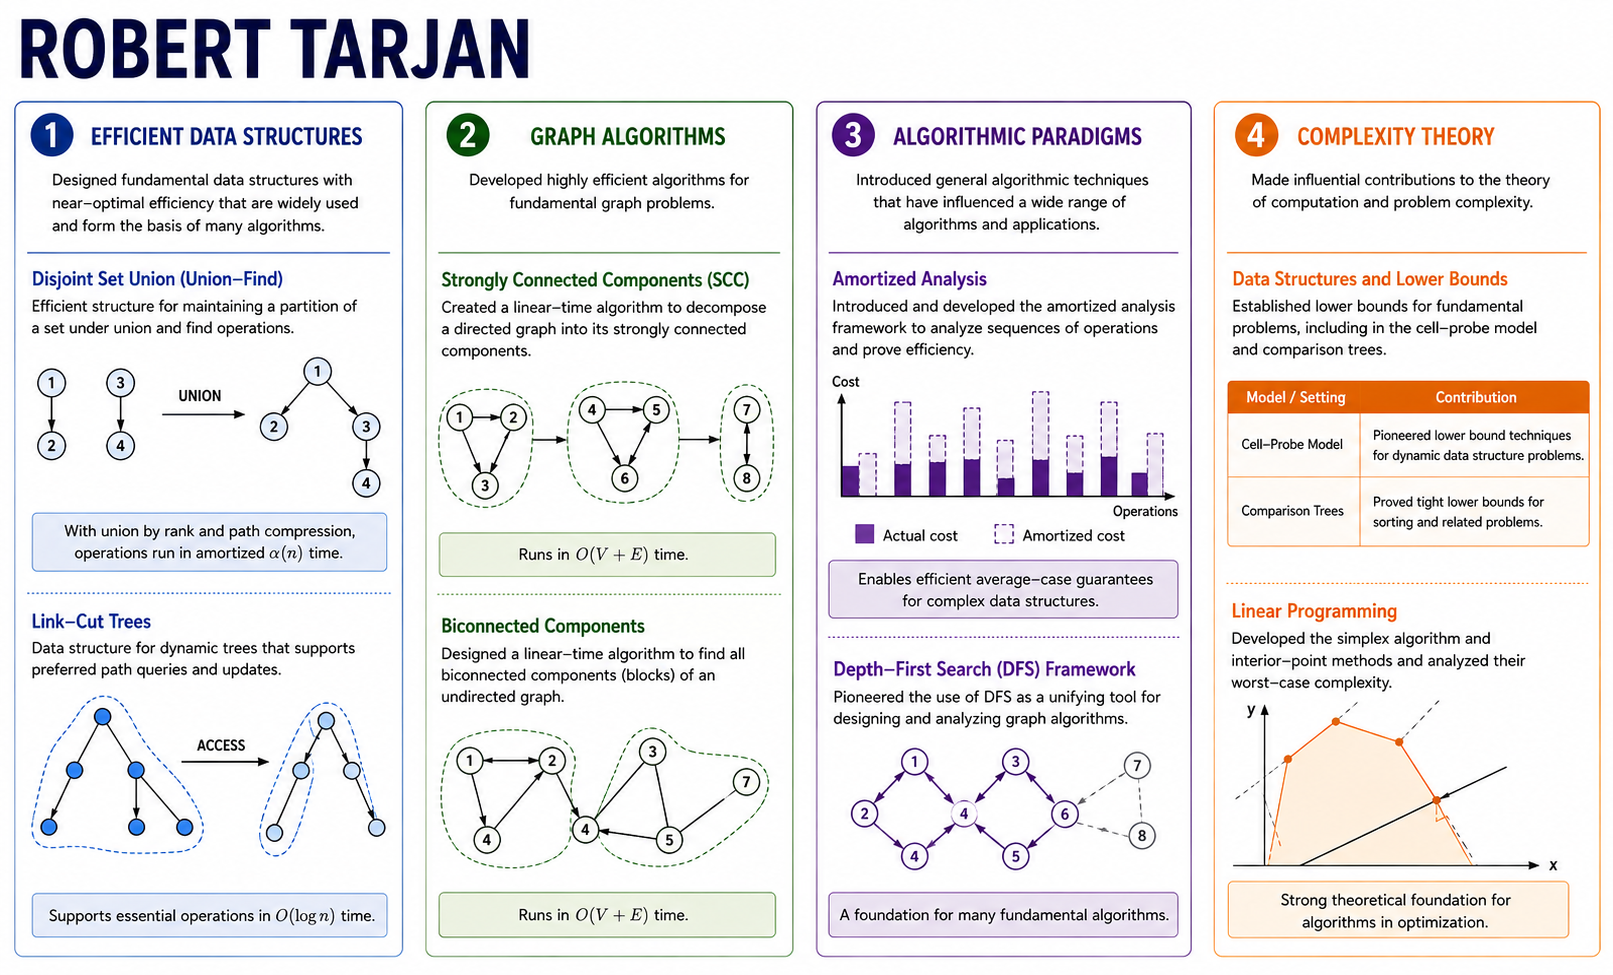
\includegraphics[width=\textwidth]{infographics/abacus1.png}
\end{center}
\expandedchapterspacing
\index{Tarjan, Robert Endre}
\booknote{The central habit in this chapter is to let a data structure remember the past, and to judge an algorithm over a whole \emph{sequence} of operations rather than one isolated step.}

\section{An Opening Story: Joining Clubs and Checking Roads}
Six friends---Alice, Bob, Carol, Dave, Eve, and Frank---start in six separate clubs, each with one member. They begin merging: Alice and Bob form one club, Carol and Dave form another, then Bob and Carol merge their two clubs. Now the question is asked: ``Are Alice and Dave in the same club?''

If the computer stores each club as a list of members, answering takes two list scans and an easy check. But suppose the clubs keep merging until thousands of people are involved. Every merge can force a list to be walked end to end, and every query may scan a large list. A program built this way can become unusable long before the problem itself is complicated. The simple question---who belongs to whom---hides a design decision: \emph{what information should the program remember between questions?}

The same issue appears for roads. A map of towns and roads is a \emph{graph}: points (\emph{vertices}) joined by lines (\emph{edges}). A \emph{bridge} is a road whose removal would split the map into two disconnected halves. How can we find every bridge without testing each road by hand?

Tarjan's 1982 Rolf Nevanlinna Prize recognized two answers that now appear in nearly every computer science curriculum: the \emph{union--find} data structure with amortized analysis, and \emph{depth-first search} with its discovery and low-link numbers. Both answers share one philosophy: the structure should record a small, provably correct summary of the past, and the running time should be measured over a whole sequence of operations.

\section{The Problem}
Two problems, both phrased as questions a computer must answer fast.

\noindent\textbf{Union--find.} We maintain a collection of disjoint sets of items. Two operations are allowed:
\begin{itemize}
\item \textsc{find}(x): return the name of the set containing $x$;
\item \textsc{union}(x,y): merge the sets containing $x$ and $y$.
\end{itemize}
A sequence of $m$ operations on $n$ items arrives, one after another. How much total time is needed? The naive list approach is easy but can be catastrophically slow on long sequences.

\noindent\textbf{Graph exploration.} Given a graph, find all bridges, articulation points (vertices whose removal disconnects the graph), and, for directed graphs, strongly connected components (maximal groups in which every vertex can reach every other). A correct but naive method---remove each edge and re-search---repeats a global computation $m$ times.

The problems look unrelated: one is about organizing data, the other about exploring a graph. The connection is that both were stuck because nobody had the right way to \emph{measure} cost and the right thing to \emph{remember}.

\section{The World Before}
In the early decades of computer science, memory was expensive, processors were slow, and an algorithm was typically judged by its worst-case performance on a single operation. Two consequences followed.

\noindent\textbf{Union--find as linked lists.} The natural implementation stores each set as a linked list. A \textsc{find} walks the list of the item's set; a \textsc{union} walks one list to its tail and attaches the other list. This is easy to describe and correct. But consider merging $n$ singletons into one set by always appending the whole current set to the next item: the growing list is walked once per merge, costing about $n^2/2$ steps. Each \textsc{union} is individually cheap---except when it is the $n$-th one---and every earlier merge looks fine in isolation. There was no language for saying: ``this particular operation is expensive, but that is fine because it can only happen rarely.''

\noindent\textbf{Finding bridges by deletion.} To test whether a road is a bridge, remove it and check whether the two endpoints are still connected. Repeating this for every edge of a graph with $m$ edges costs about $m$ full connectivity searches. On a large road map, that is hopeless. The naive algorithm works on paper but reveals nothing about the structure that makes some roads fragile and others not.

The missing ingredients were two ideas that seem obvious in hindsight:
\begin{enumerate}
\item \emph{Amortized analysis}: judge a sequence of operations, and let rare expensive operations be paid for by many cheap ones.
\item \emph{Reusable certificates}: a graph exploration should record exactly the information a later decision needs, not re-derive it from scratch.
\end{enumerate}

\section{The New Idea}
\subsection{Union--find: sets as shallow trees}
Store each set as a rooted tree, with every item pointing to its parent and a root pointing to itself. \textsc{find}(x) climbs from $x$ to its root and returns it. \textsc{union}(x,y) finds both roots and attaches one under the other.

Two refinements make the trees stay shallow:
\begin{itemize}
\item \textbf{Union by rank.} Each root carries a \emph{rank}, roughly the height of its tree. Always attach the smaller-rank root under the larger-rank one. This alone guarantees that every tree has height at most $\log_2 n$, so a single \textsc{find} never costs more than $O(\log n)$.
\item \textbf{Path compression.} During \textsc{find}(x), every vertex on the path from $x$ to the root is re-pointed directly at the root. The mathematical partition is unchanged---the representative is the same---but future queries along that path become one step each. The query \emph{rewrites the structure to make later work cheaper}.
\end{itemize}

The second refinement is the surprising one. A query that ``only asks a question'' actively improves the data structure. That is only safe if the improvement preserves the invariant that makes answers correct. It does: pointing a vertex at its root does not change which set any item belongs to.

\subsection{Amortized analysis: the bank account}
To understand why the combination is fast, forget single operations. Think of a bank account. Cheap operations deposit credit; an expensive operation spends the accumulated credit. An analysis is successful if we can prove the balance never goes negative.

Formally, assign a number $\Phi$ (the \emph{potential}) to the current state of the data structure. If operation $i$ costs $c_i$ and changes the potential from $\Phi_{i-1}$ to $\Phi_i$, its \emph{amortized} cost is defined as
\[
\widehat c_i=c_i+\Phi_i-\Phi_{i-1}.
\]
Summing over a whole sequence makes the potential terms telescope, so the total real cost equals the total amortized cost plus a boundary term. If the potential is nonnegative and each $\widehat c_i$ is small, the whole sequence is cheap. This is the mathematical version of the bank account: an expensive operation is charged for \emph{raising} the potential, and later cheap operations are the ones that spend it.

For union--find, the potential measures how ``squashed'' the trees are. Path compression is expensive when it flattens a long path, but it buys a large improvement in the forest; union by rank ensures that any one vertex cannot be moved into a better position too many times.

\subsection{Depth-first search: two numbers as a certificate}
Start at any vertex and follow one unexplored road at a time, turning back only when you reach a dead end. Number each vertex (\emph{disc}, for discovery time) in the order it is first reached. While searching, also record, for each vertex $v$, the number
\[
\operatorname{low}(v)=\text{the smallest discovery time reachable from the subtree under }v
\]
using tree edges followed by at most one non-tree edge. In words: \emph{how far back can this part of the map return, without retracing the parent road?} This is the undirected low-link quantity; for directed strongly connected components, Tarjan's algorithm uses a related low-link value that tracks edges to vertices still on the active search stack.

Two inequalities now read like the whole answer:
\begin{itemize}
\item if a child $w$ of $v$ has $\operatorname{low}(w)>\operatorname{disc}(v)$, then the road $v$--$w$ is a bridge (the subtree under $w$ cannot return to $v$ or above);
\item if $\operatorname{low}(w)\geq\operatorname{disc}(v)$, then removing $v$ separates that child's subtree from the rest (the subtree can return to $v$ itself, but not above it).
\end{itemize}
One pass over the graph produces all bridges and articulation points; with the directed-graph low-link variant and a stack, the same depth-first-search framework also produces strongly connected components. The discovery numbers and low-links are the certificate: they summarize an enormous family of possible return paths without listing them.

\section{How It Works: Worked Examples}
\subsection{A warm-up: amortization with a growing array}
Before union--find, see amortization on a friendlier object. A dynamic array must grow when it is full. Doubling the size and copying every item costs $O(n)$ when the array holds $n$ items, which sounds expensive. But over $m$ appends, the array doubles only about $\log_2 m$ times, and the total copying is
\[
1+2+4+\cdots+2^{\lceil\log_2 m\rceil}=O(m).
\]
The expensive rebuilds are paid for by the many cheap appends that filled the old block. Each append has amortized cost $O(1)$. This is the same accounting that makes path compression work.

\subsection{Union--find on six people, step by step}
Start with $A,B,C,D,E,F$, each in its own set.

\begin{enumerate}
\item \textsc{union}(A,B): both roots have rank $0$; attach $A$ below $B$. Tree: $A\to B$.
\item \textsc{union}(C,D): similarly, $C\to D$.
\item \textsc{union}(B,D): roots $B$ and $D$ have equal rank; attach $B$ below $D$. Now $A\to B\to D$ and $C\to D$. Root: $D$.
\item \textsc{find}(A): climb $A\to B\to D$ and return $D$. Path compression re-points $A$ and $B$ directly at $D$. The next \textsc{find}(A) or \textsc{find}(B) costs one step.
\item \textsc{union}(E,F): $E\to F$.
\item \textsc{find}(A) vs.\ \textsc{find}(E): returns $D$ and $F$---different clubs.
\end{enumerate}

Without path compression, step 4 would leave the chain $A\to B\to D$ intact forever. With it, the query paid for a permanent shortcut. If a club merge later asks for \textsc{find}(A) a hundred times, the first costs three steps and the remaining ninety-nine cost one each.

\subsection{A bridge hunt with depth-first search}
Take the graph with edges
\[
(a,b),(b,c),(c,a),(c,d),(d,e),(e,f),(f,d).
\]
Explore from $a$, always taking the alphabetically first unexplored road.

\begin{center}
\begin{tabular}{lcc}
\toprule
Vertex & \textsc{disc} & \textsc{low} \\
\midrule
$a$ & 1 & 1 \\
$b$ & 2 & 1 \\
$c$ & 3 & 1 \\
$d$ & 4 & 4 \\
$e$ & 5 & 4 \\
$f$ & 6 & 4 \\
\bottomrule
\end{tabular}
\end{center}

How the low-links are computed, from the leaves upward. Vertex $f$ has a back edge to $d$ (discovery time 4), so $\operatorname{low}(f)=4$. Vertex $e$ sees its child $f$ reaching 4, so $\operatorname{low}(e)=4$. Vertex $d$'s subtree reaches 4 and no further, so $\operatorname{low}(d)=4$. Vertex $c$ has a back edge to $a$ (time 1), so $\operatorname{low}(c)=1$, and this value propagates up through $b$.

Now test the bridges:
\begin{itemize}
\item edge $c$--$d$: is $\operatorname{low}(d)=4>\operatorname{disc}(c)=3$? Yes. The subtree $\{d,e,f\}$ cannot return above $c$---bridge. This matches intuition: the triangle on $a,b,c$ and the cycle on $d,e,f$ are joined only by $c$--$d$.
\item edge $e$--$f$: $\operatorname{low}(f)=4>\operatorname{disc}(e)=5$? No. Within a cycle, no single road is a bridge.
\end{itemize}
The search never tests every alternative route. It asks, once per tree edge, whether the child's subtree can climb back over the parent road. The two numbers $\operatorname{disc}$ and $\operatorname{low}$ contain exactly the information needed and no more.

\section{The Mathematics in Brief}
The famous union--find guarantee is
\[
O(m\,\alpha(n))
\]
for $m$ operations on $n$ items, where $\alpha$ is the \emph{inverse Ackermann function}. This function grows so slowly that it is at most $4$ for any number of atoms in the universe. The notation is a compact record of a real theorem: the total pointer changes across all unions and finds are almost linear. The proof groups vertices by rank and shows that a vertex can be redirected only through a tiny hierarchy of rapidly expanding rank classes. The intuition is simple even when the hierarchy is not: \emph{every expensive flattening buys a large, durable improvement in the vertex's future position.}

For depth-first search, the inequalities
\[
\operatorname{low}(w)>\operatorname{disc}(v)\quad\Longrightarrow\quad \text{edge }v\text{--}w\text{ is a bridge}
\]
and
\[
\operatorname{low}(w)\geq\operatorname{disc}(v)\quad\Longrightarrow\quad v\text{ is an articulation point for that branch}
\]
turn a visual idea about fragile networks into a checkable algorithm. The strict versus non-strict inequality is exactly the difference between ``the subtree can return to $v$ but not above it'' and ``it cannot even reach $v$ again.''

Depth-first search also produces certificates for directed graphs. A stack holds vertices of the search branch currently being explored. When a vertex is identified as the root of a strongly connected component (its low-link equals its discovery time), popping until the root removes exactly one complete component. Each vertex and edge is pushed, inspected, and removed a bounded number of times, so the whole algorithm runs in linear time.

\section{Limits and Modern Views}
The classical guarantees depend on implementation details. A careless union rule creates tall trees and destroys the near-linear bound. If parallel edges are stored without identifiers, a bridge test can mistake one copy of a doubled road for the parent edge. Recursive depth-first search can exhaust the call stack on a very long path; an iterative version must store its own exploration state. The lesson is that the invariant must be stated before the code is written.

Two modern settings push beyond the classical picture:
\begin{itemize}
\item \textbf{Dynamic graphs.} Real networks change: a road closes, a dependency is deleted. Re-running a linear algorithm after every update is too slow. Deletions are the hard case because an edge that once supported connectivity can vanish. The low-link invariant does not survive a deletion automatically, so dynamic connectivity maintains richer structures---spanning forests, balanced trees, randomized sampling---while asking the same Tarjan-style question: \emph{what summary of the past is enough to repair the answer after a local change?}
\item \textbf{Parallelism.} Depth-first search is sequential in its purest form, because the next branch depends on which vertices are already marked. Connectivity and union operations parallelize better, but synchronization and memory traffic become part of the real cost. An asymptotically optimal algorithm can lose to a worse one on real hardware if its operations are hard to distribute.
\end{itemize}

The design philosophy survives all these changes: use a small, explicit certificate of the past to make a large future computation cheap. The certificate may be a parent pointer, a rank, a discovery time, or a low-link value. Its power comes from the proof that it is exactly the information later decisions require \cite{tarjan-union,tarjan-dfs}.

\section{Exercises and Self-Study Guide}
\begin{enumerate}[label=\textbf{E\arabic*.}]
\item Run \textsc{union} by rank and \textsc{find} with path compression on the people $A,B,C,D,E,F$ with merges $(A,C)$, $(E,D)$, $(B,F)$, $(C,D)$, $(F,A)$. Draw the forest after each merge.
\hint{Attach the smaller-rank root under the larger; remember that path compression happens only inside \textup{\textsc{find}}.}
\item Show that merging $n$ singletons into one set by the linked-list method can cost about $n^2/2$ steps.
\hint{Keep merging the growing list into the next singleton, and count how many times the growing list is walked.}
\item Prove, from the low-link definition, that $\operatorname{low}(w)>\operatorname{disc}(v)$ forces the tree edge $v$--$w$ to be a bridge.
\hint{If removing $v$--$w$ still left the graph connected, some path from the subtree under $w$ to the outside would exist; trace how low-link would then reach $\operatorname{disc}(v)$ or less.}
\item On the graph $(a,b),(b,c),(c,a),(c,d)$, run depth-first search from $a$ and compute all discovery and low-link numbers. Where is the articulation point?
\hint{Follow the same table format as the worked example. Check which child $w$ of $c$ satisfies $\operatorname{low}(w)\geq\operatorname{disc}(c)$.}
\item Design a potential function that proves the amortized $O(1)$ append cost of a doubling array.
\hint{Let the potential be the number of occupied slots beyond half the array's capacity.}
\item Kruskal's minimum-spanning-tree algorithm accepts edges from lightest to heaviest, adding an edge exactly when its endpoints lie in different components. Explain which two invariants prove correctness and which data structure provides the speed.
\hint{Separate ``the accepted edges form a forest'' from ``each accepted edge is the lightest across a cut.'' Union--find maintains only the component information the first invariant needs.}
\end{enumerate}

\booknote{A final exercise in judgment: whenever a query operation improves the structure for the future, check which invariant guarantees the improvement is invisible to the answers. If you cannot name that invariant, the optimization is not safe.}
\clearpage

\chapter{1986:Leslie Valiant}
\label{chap:valiant}
\begin{center}
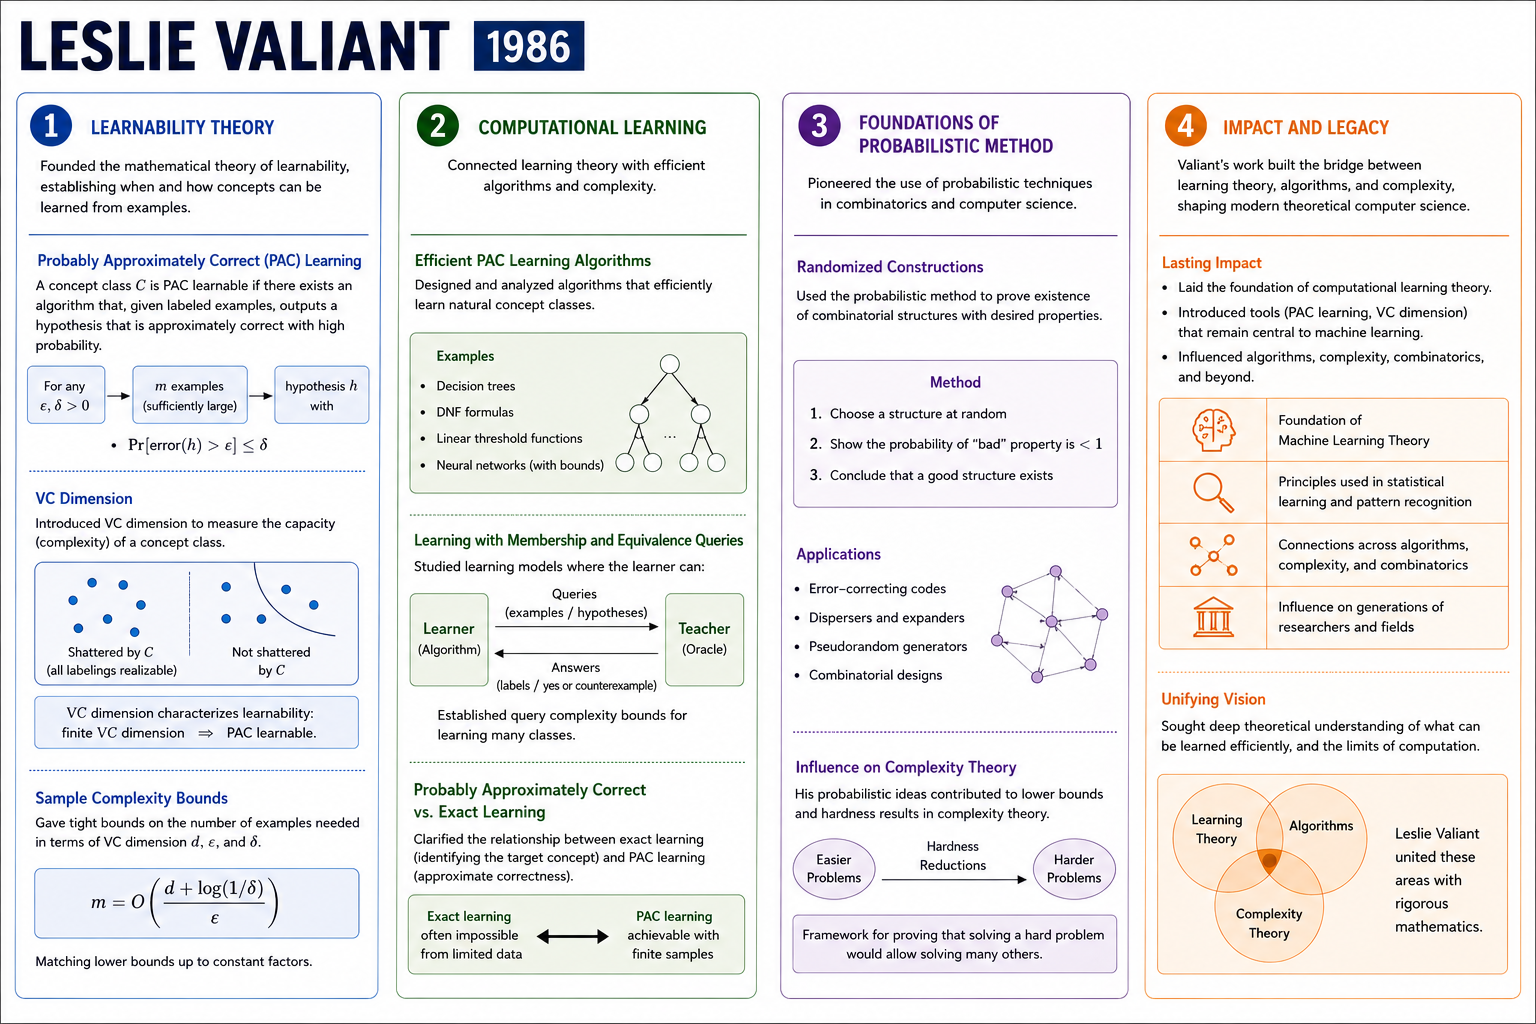
\includegraphics[width=\textwidth]{infographics/abacus2.png}
\end{center}
\longchapterspacing
\index{Valiant, Leslie}
\booknote{The central habit in this chapter is to count the witnesses, not merely to decide that one exists, and to judge a learner by a proven promise about unseen examples rather than by its score on the examples it has already seen.}

\section{An Opening Story: Pairing Up for a Quiz Night}
A quiz club has four members---Alice, Ben, Chen, and Dana---who must form two teams of two for a friendly round. There is one house rule: two members who have already been teammates this month may not pair up again. Only Alice and Ben have played together so far.

The captain asks the obvious question: ``Can we form the two teams at all?'' The answer is one bit: yes. Then the captain asks a quieter question: ``\emph{How many} different ways are there to split the four members into two allowed teams?'' The answer is a number. The full pairings of four people are (Alice,Ben)$+$(Chen,Dana), (Alice,Chen)$+$(Ben,Dana), and (Alice,Dana)$+$(Ben,Chen)---three in total. The first is forbidden, so exactly two survive. The computer had to say \emph{2}, not merely ``yes,'' and it would have had to distinguish 2 from 1 or 3 with equal care. Now grow the club: with 40 members and no restrictions, the number of ways to split into 20 teams is about \(3.2\times10^{23}\), larger than all the stars of the Milky Way, even though ``does any split exist?'' is still answered by one word. The questions look identical but are different computations: one produces a bit, the other a number that can be astronomically large.

This chapter is the mathematics of answering the second kind of question, and of a parallel discovery about learning: the same discipline that separates ``is there one?'' from ``how many are there?'' also separates ``does it fit?'' from ``will it generalize?''

\section{The Problem}
\noindent\textbf{Counting versus deciding.} A \emph{bipartite graph} is a collection of points split into two sides, left \(L\) and right \(R\), with lines (\emph{edges}) joining only left to right. A \emph{matching} is a set of edges in which no two edges share an endpoint; a \emph{perfect matching} uses every point exactly once. Think of the left side as people and the right side as jobs, an edge meaning ``this person can do this job.'' Decision asks whether every person can be assigned a distinct job; counting asks how many complete assignments exist. On a tiny instance---\(L=\{a,b,c\}\), \(R=\{1,2,3\}\), every edge present except \(a\)--\(1\)---the answers are ``yes'' and ``4.''

The same split appears in logic. A \emph{Boolean formula} is a recipe built from variables that are each true or false. The formula \(\varphi=(x\vee y)\wedge(x\vee z)\) over the variables \(x,y,z\) is true for exactly 5 of the 8 possible truth choices. ``Is there any satisfying choice?'' has answer \emph{yes}; ``how many are there?'' has answer \emph{5}.

Why should the second be harder than the first? Because a search can stop the moment it finds one witness, while a count must account for every branch, including those that contain no witness at all. To find a perfect matching you grow an assignment edge by edge, backtracking when a road closes; but backtracking records only ``this branch failed,'' discarding how many completions it contained. The count is a global property of the whole input; each local yes/no answer reveals almost nothing about it.

\noindent\textbf{Learning a rule from examples.} A learner receives examples of the form (features, label). A concrete case: a course records, for each student, the hours studied and whether the student passed. The learner wants a rule---say, a threshold on hours---that predicts the label of the \emph{next} student, who is unseen. Fitting is the easy part: any threshold that agrees with the examples is a candidate. The hard part is a promise about the future: what could justify a statement like ``with 76 examples, any threshold that fits them all misclassifies at most 10 in every 100 new cases, with 95\% confidence''? That claim concerns data never observed, so fitting cannot verify it; it needs a model in which ``generalizes'' has a precise meaning and can be proved.

\section{The World Before}
In the 1970s, Cook and Levin proved that ``does this Boolean formula have a satisfying assignment?'' is the hardest of a whole family of decision problems, and Karp exhibited dozens more with the same status. The central object of the new theory was the \emph{decision problem}: a set of inputs whose answer is yes or no. Complexity was measured by the difficulty of telling yes apart from no, and in the same decade Edmonds showed the matching problem easy for \emph{decision}: polynomial-time algorithms say whether a perfect matching exists and return one if it does.

Because decision was the currency of the field, ``solving'' a problem came to mean finding a single witness, and the folklore reflex for a count was to run the decision procedure repeatedly. This fails even in miniature. For the formula \(\varphi=(x\vee y)\wedge(x\vee z)\), a decision oracle answers ``yes,'' and each time you ask again it returns one witness, say \((1,0,0)\), then another; each answer is a single object. To learn that five exist, you must stop the oracle repeating itself by feeding back what you have already seen---bookkeeping that is enumeration, the counting computation itself. An oracle that answered ``are there at least \(k\)?'' could binary-search the count, but answering ``at least \(k\)?'' is itself a counting question.

Learning was in a similar state, but murkier. The folk model was curve fitting: take a few data points and draw a rule through them. A polynomial can pass through any finite set of points and then go anywhere at all; fitting was never the issue, so nobody could say what was being asked. Statisticians had heuristics---model selection, cross-validation, bias--variance trade-offs---but their claims were not theorems with explicit parameters.

Two conceptual tools were missing. First, a complexity theory for \emph{counting functions} rather than languages, with reductions that preserve the number of witnesses rather than merely the answer to a yes/no question. Second, a mathematical model of learning in which the error, the confidence, the number of examples, and the running time all appear as quantities in a single theorem. Valiant supplied both.

\section{The New Idea}
The first idea: \emph{count the witnesses, and treat the count as a function in its own right.} Suppose \(R(x,y)\) means ``\(y\) is a valid witness for input \(x\)'' with two constraints: each witness has length at most polynomial in the size of \(x\), and checking \(R(x,y)\) takes polynomial time. Define
\[
F_R(x)=\bigl|\{y:\lvert y\rvert\le q(\lvert x\rvert),\,R(x,y)\}\bigr|
\]
for some polynomial \(q\). The family of all such functions is \(\#\mathrm{P}\), read ``sharp P'': the functions that count efficiently checkable, polynomially bounded witnesses. Satisfying assignments, perfect matchings, and schedules all fit this form. The conceptual shift is sharp: \emph{before}, complexity theory studied sets and asked whether an input belongs to one; \emph{the new idea} is that ``how many witnesses does this input have?'' is a different question, whose answer is a possibly enormous integer. Such \emph{parsimonious} reductions---the counting analogue of polynomial-time reductions---must preserve that integer exactly, and they build a hierarchy whose top, \(\#\mathrm{SAT}\) and the \emph{permanent}, is \(\#\mathrm{P}\)-complete.

The permanent is the canonical hard counting function:
\[
\operatorname{perm}(A)=\sum_{\pi\in S_n}\prod_{i=1}^n A_{i,\pi(i)}.
\]
For a zero-one matrix it counts perfect matchings of a bipartite graph. Compare it with the determinant: the same sum, but with a sign \(\operatorname{sgn}(\pi)\) in front of every term. The sign lets elimination cancel most of the sum, which is why determinants run in polynomial time; the permanent has no cancellation, and Valiant proved it \(\#\mathrm{P}\)-complete. A single bit of information---which sign to attach---separates easy from believed-hard.

The second idea, for learning, is an explicit contract rather than a new complexity class. In the \emph{Probably Approximately Correct} (PAC) model, examples are drawn independently from an unknown distribution \(D\). The learner picks a hypothesis \(h\) from a class \(H\), and the guarantee is: with probability at least \(1-\delta\) over the sample, the probability that \(h\) errs on a fresh draw is at most \(\varepsilon\). Both the sample size \(m\) and the running time are charged. \emph{Before}, people thought learning was fitting; \emph{the new idea} is that learning is a theorem of the form ``with \(m\) samples, whatever hypothesis the algorithm chooses is good,'' where the key move is to prove the guarantee for \emph{all} hypotheses in \(H\) simultaneously---because the chosen one depends on the sample, it cannot be certified after the fact.

\section{How It Works: Worked Examples}
\subsection{Counting perfect matchings, line by line}
Take \(L=\{a,b,c\}\), \(R=\{1,2,3\}\), and every edge except \(a\)--\(1\). A perfect matching pairs each left point with a distinct right point, so it is exactly a permutation of \(\{1,2,3\}\) with \(a\) not paired with 1. Enumerate:

\begin{center}
\begin{tabular}{lccc}
\toprule
matching & assignment & uses \(a\)--1? & allowed? \\
\midrule
\(a\)--1, \(b\)--2, \(c\)--3 & 123 & yes & no \\
\(a\)--1, \(b\)--3, \(c\)--2 & 132 & yes & no \\
\(a\)--2, \(b\)--1, \(c\)--3 & 213 & no & yes \\
\(a\)--2, \(b\)--3, \(c\)--1 & 231 & no & yes \\
\(a\)--3, \(b\)--1, \(c\)--2 & 312 & no & yes \\
\(a\)--3, \(b\)--2, \(c\)--1 & 321 & no & yes \\
\bottomrule
\end{tabular}
\end{center}

Of the \(6=3!\) permutations, the two using the missing edge are discarded, leaving 4. The decision answer is ``yes,'' one bit; the count must tell this graph, with its 4 perfect matchings, apart from a graph with 1, 2, or 6. A decision algorithm returns a single matching and stops; to reach the number 4 it would have to find all four without repeating one---maintaining the list it has already produced, the counting work in disguise.

\subsection{The satisfying assignments of a tiny formula}
For \(\varphi=(x\vee y)\wedge(x\vee z)\), test all 8 assignments:

\begin{center}
\begin{tabular}{ccccc}
\toprule
\(x\) & \(y\) & \(z\) & \((x\vee y)\) & \((x\vee y)\wedge(x\vee z)\) \\
\midrule
0 & 0 & 0 & 0 & 0 \\
0 & 0 & 1 & 0 & 0 \\
0 & 1 & 0 & 0 & 0 \\
0 & 1 & 1 & 1 & 1 \\
1 & 0 & 0 & 1 & 1 \\
1 & 0 & 1 & 1 & 1 \\
1 & 1 & 0 & 1 & 1 \\
1 & 1 & 1 & 1 & 1 \\
\bottomrule
\end{tabular}
\end{center}

The count is 5. A more instructive way to see it: split on \(x\). If \(x=1\), both clauses are already satisfied and \(y,z\) are free, giving \(2\cdot2=4\) assignments. If \(x=0\), the clauses reduce to \(y=1\) and \(z=1\), giving exactly one. Total: \(4+1=5\). A decision search walks down one branch and stops; only an algorithm that keeps both branches and adds their counts returns 5.

\subsection{Learning a threshold, with a number attached}
Suppose the unknown rule is ``pass iff hours \(\ge 3\).'' Four samples arrive: hours 1 and 2 fail; hours 3.5 and 5 pass. The learner's class is thresholds \(x\ge t\); a natural choice, \(t=2.5\), sits just past the largest negative example and fits the sample, but so does \(t=3.1\). The two hypotheses differ exactly in the strip between 2.5 and 3.1, which the sample never shows. In general, a consistent threshold can err only inside the \emph{gap} between the largest negative and the smallest positive sample point, and its risk is at most the probability mass of that gap.

Now suppose the learner restricts itself to \(N=100\) candidate thresholds, so the class is finite. Fix one candidate whose true error is at least \(\varepsilon=0.1\). The probability that it makes no mistake on \(m\) random samples is at most
\[
(1-\varepsilon)^m\le e^{-\varepsilon m}.
\]
By the union bound, the probability that \emph{some} candidate is bad and yet fits the sample is at most \(100\,e^{-\varepsilon m}\). Forcing this below \(\delta=0.05\) gives
\[
m\ge\frac{1}{\varepsilon}\ln\frac{N}{\delta}=10\ln 2000\approx 76.
\]
So about 76 samples suffice: with probability at least 95\%, every candidate threshold that fits the sample has true error at most 10\%, and therefore so does the one the learner chose. The bound is \emph{uniform}---proved for all 100 candidates before the sample is drawn---so it covers whichever hypothesis the data selects; a non-uniform argument would be circular, because the chosen hypothesis is a random function of the very sample used to evaluate it.

\section{The Mathematics in Brief}
A function \(F\) belongs to \(\#\mathrm{P}\) when \(F(x)=\abs{\{y:\lvert y\rvert\le q(\lvert x\rvert),\,R(x,y)\}}\) for a polynomial \(q\) and a relation \(R\) checkable in polynomial time: the value counts \emph{witnesses}, and both the witness length and the checking time are polynomially bounded. A \emph{parsimonious reduction} maps instances of one counting problem to instances of another so that the number of witnesses is preserved exactly; \(\#\mathrm{SAT}\) and the permanent are \(\#\mathrm{P}\)-complete. Why is the permanent \(\#\mathrm{P}\)-complete? Valiant reduced \(\#\mathrm{SAT}\) to the permanent by way of \emph{cycle covers}. The permanent of the adjacency matrix of a directed graph with edge weights \(0,\pm1\) sums, over all ways to cover the vertices with disjoint directed cycles, the product of the weights on those cycles---a sum of exactly the right shape to simulate counting. Each Boolean variable becomes a small gadget with exactly two surviving local configurations, recording its truth value; each clause becomes a gadget whose cycles survive precisely for the assignments that satisfy it. The graph is built so that the only nonzero cycle covers correspond one-for-one with satisfying assignments, making the permanent equal the count. Hence a polynomial-time permanent algorithm would compute \(\#\mathrm{SAT}\), and hardness has teeth: by Cook--Levin it would put satisfiability (ask whether the count is zero) in polynomial time, and Toda's theorem extends the reach of a single counting computation beyond the whole polynomial hierarchy. Yet the difficulty is really about magnitude, not about the objects: the permanent and determinant are identical except for signs, and since \(-1\equiv 1\pmod 2\), the parity of the number of perfect matchings is computable in polynomial time as a determinant. Counting mod 2 is easy; counting exactly is believed impossible.

The PAC guarantee has the structure
\[
\text{true error}(h)\;\le\;\text{training error}(h)+\text{complexity penalty}.
\]
For a finite class of size \(N\), the penalty carries a \(\ln N\) term; the bound \(m\ge\frac1\varepsilon\ln\frac N\delta\) follows from the union bound---for a fixed hypothesis with true error at least \(\varepsilon\), the chance it looks perfect on \(m\) samples is at most \(e^{-\varepsilon m}\), multiply by the number of hypotheses, and solve for \(m\). The empirical picture transfers to new data \emph{simultaneously for the whole class}, which makes it valid for a hypothesis chosen by looking at the sample.

\section{Limits and Modern Views}
Exact counting of witnesses is believed impossible in polynomial time, so modern work asks what can be saved. One line, \emph{approximate counting}, accepts a multiplicative estimate and uses Markov chains: design a random walk whose stationary distribution weights each matching correctly, let it mix, and average an observable over the walk. This replaces the impossible exact count with a sampler, but only when the chain mixes fast. The permanent admits a fully polynomial-time randomized approximation scheme for nonnegative matrices (Jerrum, Sinclair, and Vigoda), and the subject is haunted by \emph{bottlenecks}: a chain whose state space is two dense regions joined by a narrow corridor takes exponentially long to cross it. Sampling, counting, and the geometry of the state space are one theorem.

The PAC model has aged in two ways. It is a worst-case guarantee over distributions: it holds for any \(D\), which is honest but demands more than practice needs, so modern learning theory adds structure---VC dimension replaces \(\ln N\) for infinite classes, noise and robust estimation change the loss, privacy budgets a new resource. And PAC is only the \emph{statistical} clause of learning. A hypothesis class can be statistically learnable while no efficient algorithm finds the hypothesis, and a rule that generalizes under \(D\) can fail when the future differs from the past. Valiant's insistence that error, confidence, samples, and running time be accounted together remains the frame in which all these refinements are stated \cite{valiant-counting,valiant-learning}.

\section{Exercises and Self-Study Guide}
\begin{enumerate}[label=\textbf{E\arabic*.}]
\item Verify by listing: how many assignments of \((x,y,z)\in\{0,1\}^3\) satisfy \((x\vee y)\wedge(y\vee z)\wedge(z\vee x)\)?
\hint{Only four of the eight assignments are excluded. Group the exclusions by which pair of variables is both 0.}
\item In the worked matching graph, remove a second edge, \(b\)--\(2\), in addition to \(a\)--\(1\). Count the perfect matchings using inclusion--exclusion.
\hint{Start from \(3!=6\). The 2 matchings using \(a\)--\(1\) and the 2 using \(b\)--\(2\) overlap in the 1 matching using both, so \(6-2-2+1=3\).}
\item Give a counting problem whose decision version is easy but whose count is believed hard, and explain why calling the decision algorithm repeatedly does not help.
\hint{2-satisfiability is solvable in polynomial time, yet counting its satisfying assignments is \(\#\mathrm{P}\)-complete.}
\item Derive the union-bound sample size \(m\ge\frac1\varepsilon\ln\frac N\delta\) from scratch, and re-check the number 76.
\hint{Fix one hypothesis with true error at least \(\varepsilon\); bound the chance that it is clean on \(m\) samples by \(e^{-\varepsilon m}\); union over all \(N\) and solve for \(m\).}
\item Give two thresholds that agree on the sample \(\{1,2,3.5,5\}\) but disagree on an unseen region, and state what extra information would distinguish them.
\hint{Any \(t\in(2,3.5]\) is consistent with the sample; two such thresholds differ on the strip between them, where the risk lives.}
\item Describe a Markov chain whose states are the perfect matchings of a small bipartite graph, and draw a graph for which the chain has a clear bottleneck.
\hint{Let a step move to a new matching by toggling one or two edges, with proposal probabilities chosen to keep the chain symmetric; a bottleneck is two large families of matchings joined by very few intermediate matchings.}
\item Take the claim ``a learner trained on these examples will generalize.'' Separate it into a statistical clause, a computational clause, and a robustness clause, and say which one the PAC theorem actually proves.
\hint{The theorem proves the statistical clause under the assumption that samples are independent draws from a fixed distribution; the computational clause concerns the algorithm's running time, and the robustness clause concerns what happens if the future distribution differs.}
\end{enumerate}

\booknote{A final exercise in judgment: whenever someone hands you a number that claims to describe how many, or a learner that claims to have generalized, ask which parts of the claim are theorems, which parts are assumptions, and which parts are hope---and state what data, or what reduction, would have to exist to convert each hope into a theorem.}
\clearpage

\chapter{1990:Alexander A. Razborov}
\label{chap:razborov}
\targetchapterspacing
\index{Razborov, Alexander A.}
\booknote{The central habit in this chapter is to prove a universal negative: find a quantity that every allowed gate changes only a little, so every small circuit is trapped in a box the target function can escape.}

\section{An Opening Story: The Proof Game}
Three switches guard a vault door, which opens only when all three are on. You build the obvious controller: two AND gates, one combining switches 1 and 2, the second combining that with switch 3. Done. Now a skeptic enters. ``You found one circuit,'' she says. ``Prove that \emph{no} circuit with a single two-input gate can open the vault.''

A single gate reads at most two switches and ignores the third, so the output cannot react to it---the claim is easy. So she makes it harder: five switches, the door opens exactly when at least three are on, and she wants a certificate that no circuit with, say, seven gates can do the job. No single gate ignores enough inputs, and no obvious trick works. This is the \emph{proof game}: one player claims a rule is easy, the other must rule out \emph{every} circuit that might compute it, including circuits nobody has thought to write down. Alexander Razborov won the 1990 Nevanlinna Prize for winning the hard side of this game for important restricted circuits, proving that natural rules such as ``does this graph contain a large clique?'' need many gates.

\section{The Problem}
A \emph{Boolean function} is a rule $f\colon\{0,1\}^n\to\{0,1\}$ reading $n$ bits and answering one. Unless stated otherwise, a \emph{Boolean circuit} is a directed acyclic graph whose leaves are the input bits, whose internal nodes are binary AND, OR, and NOT gates, and whose top node is the output. The \emph{size} is the number of gates; the \emph{depth} is the longest path from an input to the output. We will explicitly identify models with unbounded fan-in when they are used.

The question is \emph{prove that a specific function requires many gates.} The asymmetry is brutal: an upper bound is one construction, while a lower bound must defeat \emph{all} circuits in a class---an unbounded set of objects, most never seen. Easy to find clever constructions; hard to show cleverness has a limit.

\section{The World Before}

\noindent\textbf{Counting says hard functions exist.} There are $2^{2^n}$ Boolean functions on $n$ bits---$2^{16}=65{,}536$ for $n=4$, about $10^{308}$ for $n=10$. A circuit of $s$ gates is described by naming a type and wires per gate, leaving roughly $(c\,s)^s$ circuits of size $s$; for $s=2^n/n$ this is far smaller than $2^{2^n}$. So almost all functions need about $2^n/n$ gates: hard functions are the typical case.

\noindent\textbf{But existence is not an example.} The counting argument never names a hard function. ``Most functions are hard'' and ``here is one, with a proof'' are different statements, and for decades nobody could make the second. For explicit functions the best bounds were trivial---roughly enough gates to read the input and nothing more.

\noindent\textbf{The field was rich in upper bounds.} Sorting, multiplying, matching: fast algorithms, each a triumph of construction. The discipline could answer ``how fast can it be done?'' and had almost no tools for ``how slow must it be?'' The temptation was to judge hardness by cleverness---``I could not find a circuit'' is a statement about one person, not a theorem about all circuits.

\noindent\textbf{What was missing: an invariant.} A lower bound needs a measure $\mu(f)$ with two properties: each single gate changes $\mu$ by a controlled amount, so a circuit of $s$ gates leaves $\mu$ inside a controlled range; and the target function sits far outside that range. The creative work is finding a measure that \emph{survives composition of gates}, so composing two gates cannot let it explode.

\section{The New Idea}
\emph{Step one:} choose a measure every allowed gate changes by a controlled amount. \emph{Step two:} exhibit a target whose measure is unavoidably large. Three moves make this work.

\subsection{Monotone circuits: remove the eraser}
A function is \emph{monotone} if flipping an input bit from $0$ to $1$ never flips the output from $1$ to $0$; evidence once collected cannot be forgotten. A \emph{monotone circuit} uses only AND and OR gates, no NOT. This sounds mild but removes the most dangerous power of general circuits: \emph{cancellation}. With NOT, a circuit can combine a fact with its negation, $x\wedge\neg x=0$, and erase everything it learned. Monotone circuits must keep what they collect, so a measure of ``how much evidence is held'' can survive the whole computation.

\subsection{Polynomial approximations: the stabilizer}
Even monotone gates are hard to track exactly. Razborov's key move was to replace each gate's behavior, on carefully chosen test graphs, by a low-complexity combinatorial stand-in---essentially a bounded collection of small sets or terms. The stand-in makes only a controlled number of mistakes at each gate, while the target clique function cannot be approximated accurately by any sufficiently small collection. The whole circuit is therefore trapped between two facts: local approximants are stable under AND and OR, but no small approximant can separate the relevant positive and negative graphs. Approximation is the lever that lets a counting argument reach inside the circuit.

\subsection{The clique bound: a target that resists}
The flagship target: input a graph on $n$ vertices---one bit per possible edge---and ask whether it contains $k$ vertices all pairwise connected, a $k$-\emph{clique}. This is monotone: adding edges only creates cliques. Razborov's 1985 work gave the first super-polynomial monotone-circuit lower bound for clique. Alon and Boppana later strengthened this line of work to bounds of the form $n^{\Omega(\sqrt{k})}$ over a broad range of $k$. Positive inputs carry huge numbers of incompatible witnesses, while a small circuit's approximant keeps only a limited catalogue, so some graph with no $k$-clique slips through. The conceptual shift is the whole lesson: \emph{an upper bound needs one construction; a lower bound must defeat every construction, so find the invariant all small circuits share.}

\section{How It Works: Worked Examples}

\subsection{No monotone circuit computes parity of three bits}
Let $p$ be parity of $x_1,x_2,x_3$: output $1$ for an odd number of $1$s. Then
\[
p(0,1,0)=1,\qquad p(0,1,1)=0.
\]
Flipping $x_3$ from $0$ to $1$ moved the output from $1$ to $0$: an input bit went up and the answer went down. Monotone functions never do that, so parity is not monotone. And every monotone circuit computes a monotone function: input wires are monotone, and AND or OR of monotone functions is monotone. Hence \emph{no} monotone circuit computes parity, of any size. Trivial---yet it teaches the method's point: monotonicity removes the ability to cancel. Parity needs the circuit to remember that two ones cancel, and monotone hardware has no eraser. Nor is the case moot: reachability, matching, and clique are all monotone, and these are exactly what graph circuits are asked to compute.

\subsection{AND of three bits: two models, and a measure that fails}
First, the model matters. In an unbounded-fan-in model, one 3-input AND gate computes $x_1\wedge x_2\wedge x_3$ in size $1$, depth $1$. In the binary model used by default here, the same function needs $(x_1\wedge x_2)\wedge x_3$: size $2$, depth $2$.

Now try the most naive measure: $\mu(f)=$ number of assignments where $f$ outputs $1$. Two tiny circuits show it cannot work. The four-way OR $x_1\vee x_2\vee x_3\vee x_4$ takes three binary gates yet outputs $1$ on $15$ of $16$ assignments: tiny circuit, huge $\mu$. The function $x_1\wedge(x_2\vee x_3)$ takes two gates yet outputs $1$ on only $3$ of $8$. Same gate counts, opposite measures. The reason is composition: for $h$ and $g$,
\[
\mu(h\vee g)=\mu(h)+\mu(g)-\mu(h\wedge g),
\]
and the correction $\mu(h\wedge g)$ is a correlation no gate-local rule can predict. A chain of OR gates can keep $\mu$ small by exploiting overlaps, or inflate it by avoiding them. The measure does not respect composition, so it proves nothing---real measures must be \emph{provably stable} under each gate, not merely plausible.

\section{The Mathematics in Brief}
The precise objects first. A \emph{Boolean circuit} with $n$ inputs is a directed acyclic graph whose leaves are the input bits and whose internal nodes are AND, OR, and NOT gates, with one designated output; \emph{size} is the number of gates and \emph{depth} is the longest input-to-output path. A polynomial-size circuit family defines the nonuniform class $\mathrm{P}/\mathrm{poly}$, the circuit analogue of polynomial-time computation. Proving that an explicit language in $\mathrm{NP}$ requires super-polynomial general circuits would show $\mathrm{NP}\not\subseteq\mathrm{P}/\mathrm{poly}$, and therefore $\mathrm{P}\ne\mathrm{NP}$. Removing NOT gates and keeping only AND/OR gives \emph{monotone circuits}; a \emph{monotone function} satisfies $f(x)\le f(y)$ whenever $x\le y$ coordinatewise. Keeping NOT but fixing the depth at a constant, requiring polynomial size, and letting AND/OR gates read unboundedly many inputs gives $\mathrm{AC}^{0}$. The headline theorem:

\medskip
\noindent\emph{Razborov (1985), with later strengthening by Alon--Boppana (1987)} \cite{razborov-monotone,alon-boppana}. Razborov proved a super-polynomial lower bound for monotone circuits deciding whether an $n$-vertex graph contains a suitable $k$-clique. Later work established the more general form $n^{\Omega(\sqrt{k})}$ over a broad range of $k$; for $k\approx n^{1/3}$ this outgrows every fixed power of $n$.

The engine is Razborov's \emph{method of approximation}, not a generic low-degree-polynomial substitution. On a carefully selected collection of positive and negative graphs, replace the output of each gate by a bounded-complexity monotone approximant, such as a short DNF built from small vertex sets. The approximant for each gate makes only a controlled number of errors, and the gate rules ensure that these errors cannot disappear without being charged to earlier gates. At the output, however, every small approximant must confuse a graph containing a genuine $k$-clique with a graph whose largest clique is much smaller. The local and global error bounds contradict one another unless the original circuit has many gates. Low-degree polynomial approximation is an important related technique in other circuit lower bounds, but it should not be presented as the mechanism of this monotone clique proof.

The general question---an explicit function needing super-polynomial \emph{general} circuits---remains open: negation reintroduces cancellation, and $x\wedge\neg x=0$ destroys every known measure.

\section{Limits and Modern Views}
Monotone circuits are a restricted model, and the restriction does the work. General circuits can cancel, forget, and coordinate globally; the measures that defeat monotone circuits evaporate at the first NOT gate. Threshold gates---comparing a weighted sum $\sum_i w_i x_i$ to a threshold---add a power none of the classical invariants controls. No one has exhibited an explicit function provably requiring super-polynomial general circuits, and Razborov and Rudich's \emph{natural proofs} barrier explains part of why: assuming strong pseudorandom functions exist, no lower-bound property that is both sufficiently constructive and sufficiently large can yield the desired general-circuit lower bounds. Many promising techniques cannot resolve $\textsf{P}$ vs.\ $\textsf{NP}$; a breakthrough must be unnatural in a precise technical sense.

What survived is the method. The invariant-and-approximant pattern now appears in proof complexity (Razborov's own work on the pigeonhole principle and bounded arithmetic bounds how concisely some statements can be proved \cite{razborov-circuit}), pseudorandomness, communication complexity, and learning theory, where a ``small approximator'' is what an efficient learner must find. The 1990 Nevanlinna Prize honored the pattern, not just the clique bound \cite{razborov-monotone}: \emph{to prove a machine cannot be small, find the quantity every small machine must respect, then find a task that violates it.}

\section{Exercises and Self-Study Guide}
\begin{enumerate}[label=\textbf{E\arabic*.}]
\item Compare a balanced formula for AND of $n=8$ variables with a chain formula. Give the exact size and depth of each.
\hint{Draw both trees: a balanced binary AND tree has depth $\log_2 8=3$; a chain has depth $7$; both use $7$ gates.}
\item Prove that the parity function $p(x_1,x_2,x_3)$ is not monotone, and conclude no monotone circuit computes it.
\hint{Find two inputs differing in one bit where $p$ drops from $1$ to $0$; every AND/OR-only circuit computes a monotone function.}
\item Apply a random restriction to the majority-of-three DNF $f=(x_1x_2)\vee(x_2x_3)\vee(x_1x_3)$ by hand: first set $x_2=1$, then $x_2=0$. Which terms die, and what function remains?
\hint{Setting $x_2=1$ turns $x_1x_2$ and $x_2x_3$ into $x_1$ and $x_3$; setting $x_2=0$ kills all three terms.}
\item Explain why a lower bound for monotone circuits says nothing directly about general circuits, using AND of three bits as a test case.
\hint{The same function is cheaper in a stronger model: one 3-input AND beats any binary-circuit bound, and a NOT gate adds powers monotone circuits lack.}
\item Compute $\mu(f)$, the number of assignments where $f$ outputs $1$, for $x_1\vee x_2\vee x_3\vee x_4$ and for $x_1\wedge(x_2\vee x_3)$. Why do these numbers rule out ``small circuit implies small $\mu$''?
\hint{The four-way OR outputs $1$ on $15$ of $16$ assignments; the two-gate function on $3$ of $8$. Same gate counts, opposite measures.}
\item Prove that no circuit with a single two-input AND, OR, or NOT gate computes majority of three bits.
\hint{A one-gate circuit ignores some input $x_j$; pick two inputs differing only in $x_j$ where majority flips, e.g.\ $(0,1,0)$ vs.\ $(0,1,1)$.}
\item Read a published lower-bound proof (Razborov's monotone clique bound, or an exposition of it) and mark every place the machine model is used.
\hint{Ask the four questions: what is the model, what quantity is small for every small machine, why does it survive each gate, where does the target violate it.}
\end{enumerate}

\booknote{A final exercise in judgment: whenever you read that a circuit class cannot compute a function, name the forbidden power---cancellation, global coordination, thresholds---and ask which future gadget would make the old measure fail. Naming the next forbidden power is how lower bounds progress.}
\clearpage

\chapter{1994:Avi Wigderson}
\label{chap:wigderson}
\begin{center}
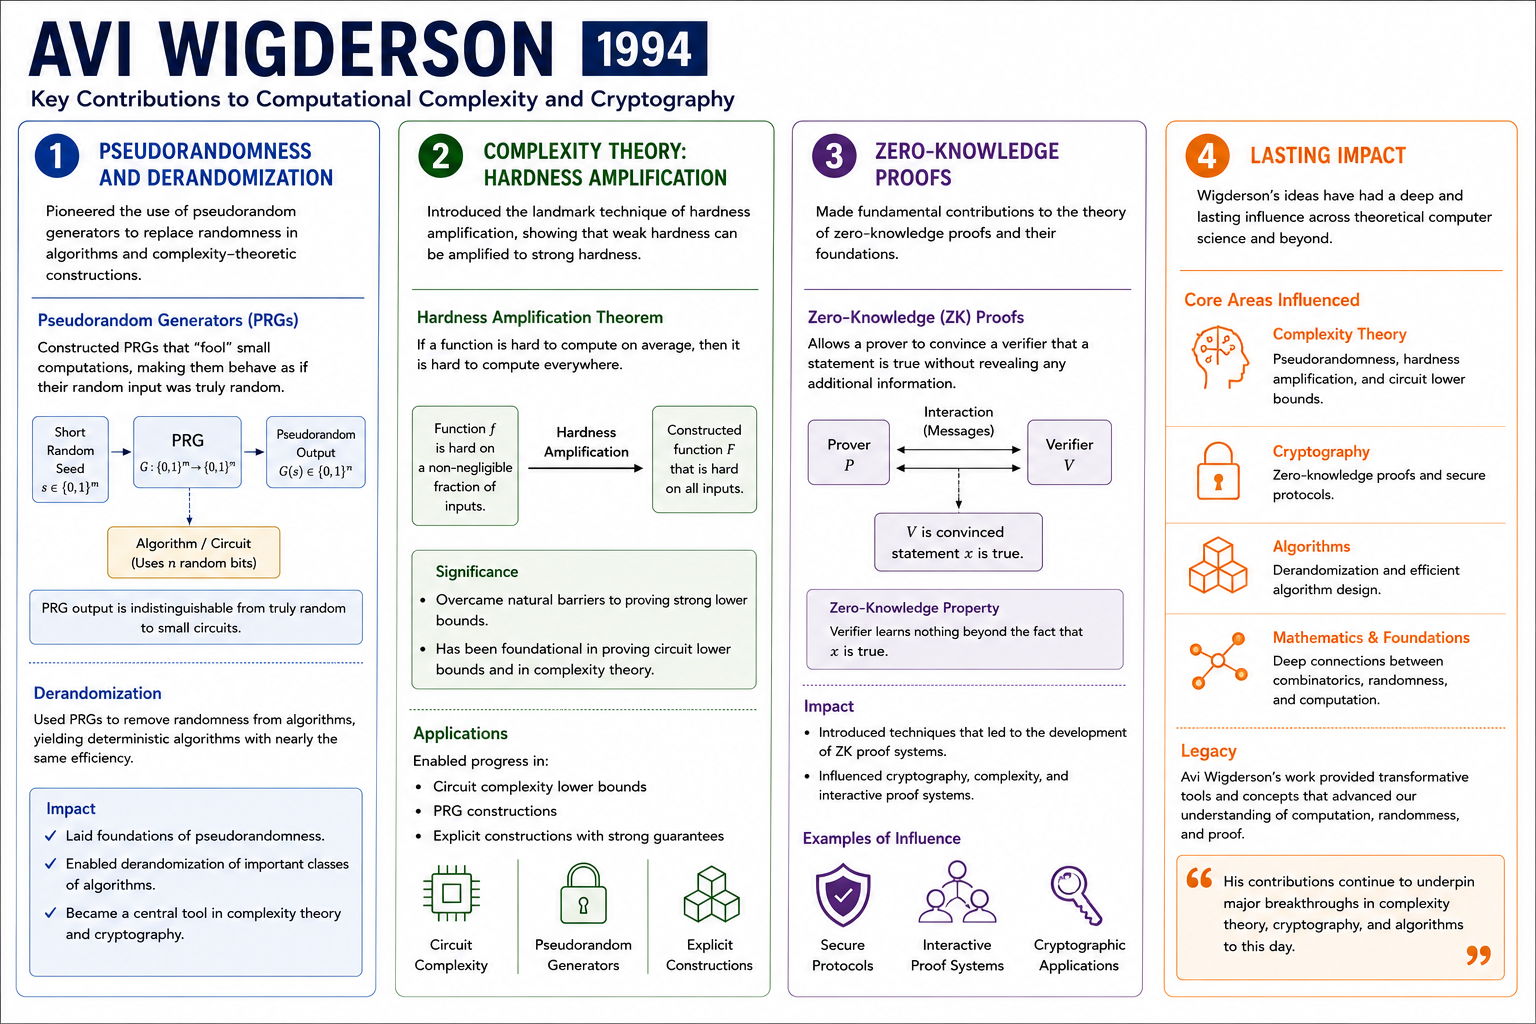
\includegraphics[width=\textwidth]{infographics/abacus4.png}
\end{center}
\targetchapterspacing
\index{Wigderson, Avi}
\booknote{The central habit in this chapter is to let a verifier's random challenge choose what to inspect, and to judge a claimant by the probability of being caught rather than by any single answer.}

\section{An Opening Story: Two Drawings and a Know-It-All}
Two cards lie on a table, each showing a graph on five dots and five lines: one is a five-cycle, the other is a triangle with a two-edge tail attached to one of its vertices. Sam claims he can always tell them apart, even after someone renames the dots.

The teacher tests him. She secretly picks a card, renames all five dots with a fresh shuffle each round, shows the result, and asks: five-cycle or triangle-plus-tail? If the graphs really differ, Sam answers correctly every round. If they secretly showed isomorphic graphs, the rename hides which card was picked and even a perfect answerer is right only half the time; ten rounds of guessing pass with probability $(1/2)^{10}<1/1000$.

Nothing was checked directly. The teacher asked a question she could not answer herself, and the shuffle made it fair: a challenge known in advance could be met with a prepared lie. Randomness turned ``these two are not the same''---a claim with no short written proof---into tests a liar cannot all pass.

\section{The Problem}
One person, the \emph{prover}, claims a fact and will do enormous work to defend it. A second, the \emph{verifier}, has little time and must decide whether to believe it. The prover might lie. How can the verifier be convinced?

The classical answer is a \emph{certificate}: a fixed string a fast deterministic algorithm checks. For ``these two drawings are the same shape'' the certificate is easy: hand over the renaming and compare. The opposite claim, ``these two are \emph{not} the same shape,'' has no known short certificate. For graphs $G_1,G_2$ this is graph non-isomorphism (GNI): an isomorphism witnesses that they \emph{are} the same, but no short static certificate of non-isomorphism is known.

The verifier cannot recompute, cannot trust, and cannot peek inside the prover's head. The escape is conversation: questions the prover could not have anticipated. \emph{Can a weak verifier be convinced of a statement with no short static certificate, by a powerful prover who might be lying?}

\section{The World Before}
For most of the history of logic, a proof was a static object: a certificate string checked mechanically. Computer science inherited this as the class NP: every yes-instance has a short certificate a deterministic verifier accepts, and no no-instance has one. ``Checking is easy, finding is hard'' was the whole vocabulary.

GNI was an embarrassment for that picture. Its no-instances---the isomorphic pairs---have short certificates, namely an isomorphism; its yes-instances have no known short static certificates. Since a certificate can only witness membership, ``not isomorphic'' looked like a problem with no proof at all.

Randomness made things worse before better: randomized algorithms were viewed as a confession of weakness, and the goal was to remove the coin flips. Nobody asked whether a verifier could \emph{use} coin flips as a resource.

What was missing was a proof as a conversation with two extra resources: \emph{interaction} (follow-up questions) and \emph{public randomness} (unpredictable coins). Without both, GNI sat outside any efficient verification framework.

\section{The New Idea}
\subsection{Conversation, not certificate}
An \emph{interactive proof} replaces the certificate with a dialogue. The prover may compute anything; the verifier flips coins, asks questions, and the prover's answer is conditioned on a challenge not known in advance. A pre-announced challenge could be met by one fixed lie; the random challenge is the whole point.

\subsection{The two promises}
\emph{Completeness}: if the claim is true, an honest prover convinces the verifier with high probability. \emph{Soundness}: if it is false, no prover, however clever, convinces it except with small probability. Both probabilities are over the verifier's coins, not the prover's goodwill. Repetition with fresh coins multiplies the error: $1/2$ becomes $(1/2)^k$, below $1/1000$ at $k=10$.

\subsection{Arithmetization: logic becomes algebra}
Rewrite a Boolean computation as polynomial equations over a finite field. A bit $x$ is forced by $x^2-x=0$; AND becomes multiplication ($x\wedge y\mapsto xy$) and OR becomes $x+y-xy$. A circuit becomes one polynomial identity, checked at a few random points.

\subsection{IP = PSPACE}
Lund, Fortnow, Karloff, Nisan, and Shamir proved that every problem solvable with polynomial memory---the class PSPACE---has an interactive proof. A conversation is as powerful as any algorithm for the problem.

\subsection{Zero knowledge: validity without the secret}
Wigderson's signature addition: prove a statement true while revealing nothing about why. A zero-knowledge proof is complete and sound and has transcripts that can be simulated without the witness; if the verifier could have produced the conversation alone, it carries no information. \emph{A proof is not an object; it is a conversation.}

\section{How It Works: Worked Examples}
\subsection{Graph non-isomorphism, round by round}
Let $G_1$ be the five-cycle and $G_2$ the triangle with a two-edge tail attached to one vertex---five vertices and five edges each, not isomorphic. One round: the verifier flips a coin, applies a uniformly random relabeling $\pi$ to the chosen graph, and sends it to the prover, who answers ``five-cycle'' or ``triangle-plus-tail.''

If the claim is true, the honest prover always identifies the graph and passes with probability $1$. If it is false---the graphs \emph{are} isomorphic---a relabeled $G_1$ and a relabeled $G_2$ come from exactly the same distribution, so the answer is independent of the coin and correct with probability $1/2$; ten rounds leave error at most $(1/2)^{10}<1/1000$. The coins matter: a fixed rename could be answered by a memorized lie; a fresh one cannot.

\subsection{Checking a polynomial identity}
The prover claims $x^2=1$ for every $x$. Over $\mathbb{F}_{101}$, the verifier picks a random $r\in\{0,\ldots,100\}$, computes $r^2$ and $1$, and checks equality. The difference $x^2-1=(x-1)(x+1)$ has exactly two roots, $x=1$ and $x=100$, so a random point exposes the lie with probability at most $2/101\approx2\%$. Three independent checks multiply the error to about $(2/101)^3<10^{-5}$.

This is the engine of arithmetization: two distinct polynomials of degree at most $d$ over a field of size $q$ agree at at most $d$ points, so one random evaluation gives meaningful evidence.

\subsection{Zero knowledge on a small graph}
A triangle $a,b,c$ is colored red, blue, red. The prover wants to prove the triangle is $3$-colorable without naming a color. Each round it picks a fresh random permutation of the colors, commits to every vertex's color (hidden until opened), and the verifier picks one of the three edges and asks to open just its two endpoints. The check: the colors differ.

A proper coloring passes every round. A lying prover with a bad edge is caught exactly when that edge is picked, with probability at least $1/3$ per round; $k$ rounds leave error at most $(2/3)^k$, about $1.7\%$ at $k=10$. Nothing leaks because each round uses a fresh permutation: the opened pair is always just ``two distinct colors from three,'' exactly what a simulator without the coloring can reproduce.

\section{The Mathematics in Brief}
An interactive proof for a language $L$ is a pair of machines exchanging messages. For an instance $x$:
\[
x\in L \Rightarrow \PP[V\text{ accepts with honest }P]\geq 2/3,
\qquad
x\notin L \Rightarrow \PP[V\text{ accepts with any }P]\leq 1/3.
\]
The gap between $2/3$ and $1/3$ is deliberate: repetition pushes the $1/3$ toward $0$ exponentially while an honest prover stays accepted. Probabilities are over the verifier's coins only.

The workhorse lemma: \emph{two distinct polynomials of degree at most $d$ over a field of size $q$ agree at at most $d$ points}---their difference is a nonzero polynomial with at most as many roots as its degree.

Arithmetization rests on three exact translations (field of characteristic not $2$):
\[
x\in\{0,1\} \Longleftrightarrow x^2-x=0,\qquad
x\wedge y \Longleftrightarrow xy,\qquad
x\vee y \Longleftrightarrow x+y-xy.
\]
A circuit becomes a system of polynomial equations; a claimed computation becomes a polynomial identity. Lund--Fortnow--Karloff--Nisan and Shamir then proved $\mathrm{IP}=\mathrm{PSPACE}$: interactive proofs capture exactly polynomial memory. Constructively: unwind the computation into a layered circuit, arithmetize it, and verify by a sum-check that justifies a multivariate sum one variable at a time.

Zero knowledge adds a simulation condition: a polynomial-time machine that, given only $x\in L$, produces transcripts indistinguishable from real ones; since it needs no witness, real transcripts cannot be milked for one. The costs are asymmetric: the prover may work exponentially, the verifier polynomially, and soundness error and randomness spent are part of the resource bill.

\section{Limits and Modern Views}
The costs are real: for GNI the prover must actually decide isomorphism, and for arithmetized computations it must manipulate polynomials the verifier never touches. The guarantee is probabilistic, not certain. Zero knowledge adds friction: commitments rest on computational assumptions, transcripts must be rechecked for leakage, and reusing randomness across rounds can destroy privacy.

The ideas outgrew their origin in three directions. \emph{Probabilistically checkable proofs} (PCPs) showed an ordinary NP certificate can be checked by reading a handful of bits---a static object with interactive power. \emph{Succinct proofs} (SNARKs, STARKs) let a cloud computer convince a laptop that a huge computation ran correctly, trading prover time against tiny proofs, amid debates about trusted setup and proof length. \emph{Post-quantum cryptography} asks whether the assumptions behind commitments and succinct proofs survive a quantum adversary, and answers with lattice problems \cite{wigderson-interactive,wigderson-zk}. The lessons persist: expose algebraic structure, sample random constraints instead of rechecking everything, and separate validity from secrecy.

\section{Exercises and Self-Study Guide}
\begin{enumerate}[label=\textbf{E\arabic*.}]
\item Write the polynomial constraint that forces a variable to be a bit, and verify it in $\mathbb{F}_3$ at $x=0,1,2$.
\hint{$x^2-x=0$; $x=2$ gives $4-2=2\neq0$, and note why the trick silently fails in $\mathbb{F}_2$.}
\item Show that $P(x)=x^2$ and $Q(x)=1$ agree at exactly two points in $\mathbb{F}_7$, and list them.
\hint{Solve $x^2=1$ over $\{0,\ldots,6\}$; the solutions are $x=1$ and $x=6$, so a random point catches the difference with probability $5/7$.}
\item A protocol has soundness error $1/3$. Find the smallest $k$ such that $k$ independent rounds bring the error below $1/100$.
\hint{$(1/3)^4=1/81$ is still above $1/100$; $k=5$ gives $1/243$.}
\item Construct a zero-knowledge transcript that accidentally reveals the witness, using the $3$-coloring protocol on the triangle.
\hint{Reuse the same color permutation in two rounds opening two edges that share a vertex; combining the opened colors pins down the full coloring.}
\item Compute the soundness error of the GNI protocol for $k=5$ rounds, and state the honest prover's acceptance probability.
\hint{$(1/2)^5=1/32\approx3\%$; the honest prover is still accepted with probability $1$.}
\item Convert the Boolean formula $(x\wedge y)\vee z$ into polynomial equations, including bit constraints.
\hint{Introduce $a=xy$ for the AND; the OR becomes $a+z-az$; each variable satisfies $t^2-t=0$.}
\item Explain why the verifier must not reveal its random challenge before the prover answers, using GNI.
\hint{A pre-announced rename is a single test with a memorized answer; randomness makes every round a fresh test.}
\end{enumerate}

\booknote{A final exercise in judgment: before trusting any verification system, name what the verifier's random coins protect against. If the answer is ``a prepared lie,'' find the challenge the prover cannot predict; if you cannot name it, the protocol is only a certificate wearing a costume.}
\clearpage

\chapter{1998:Peter W. Shor}
\label{chap:shor}
\begin{center}
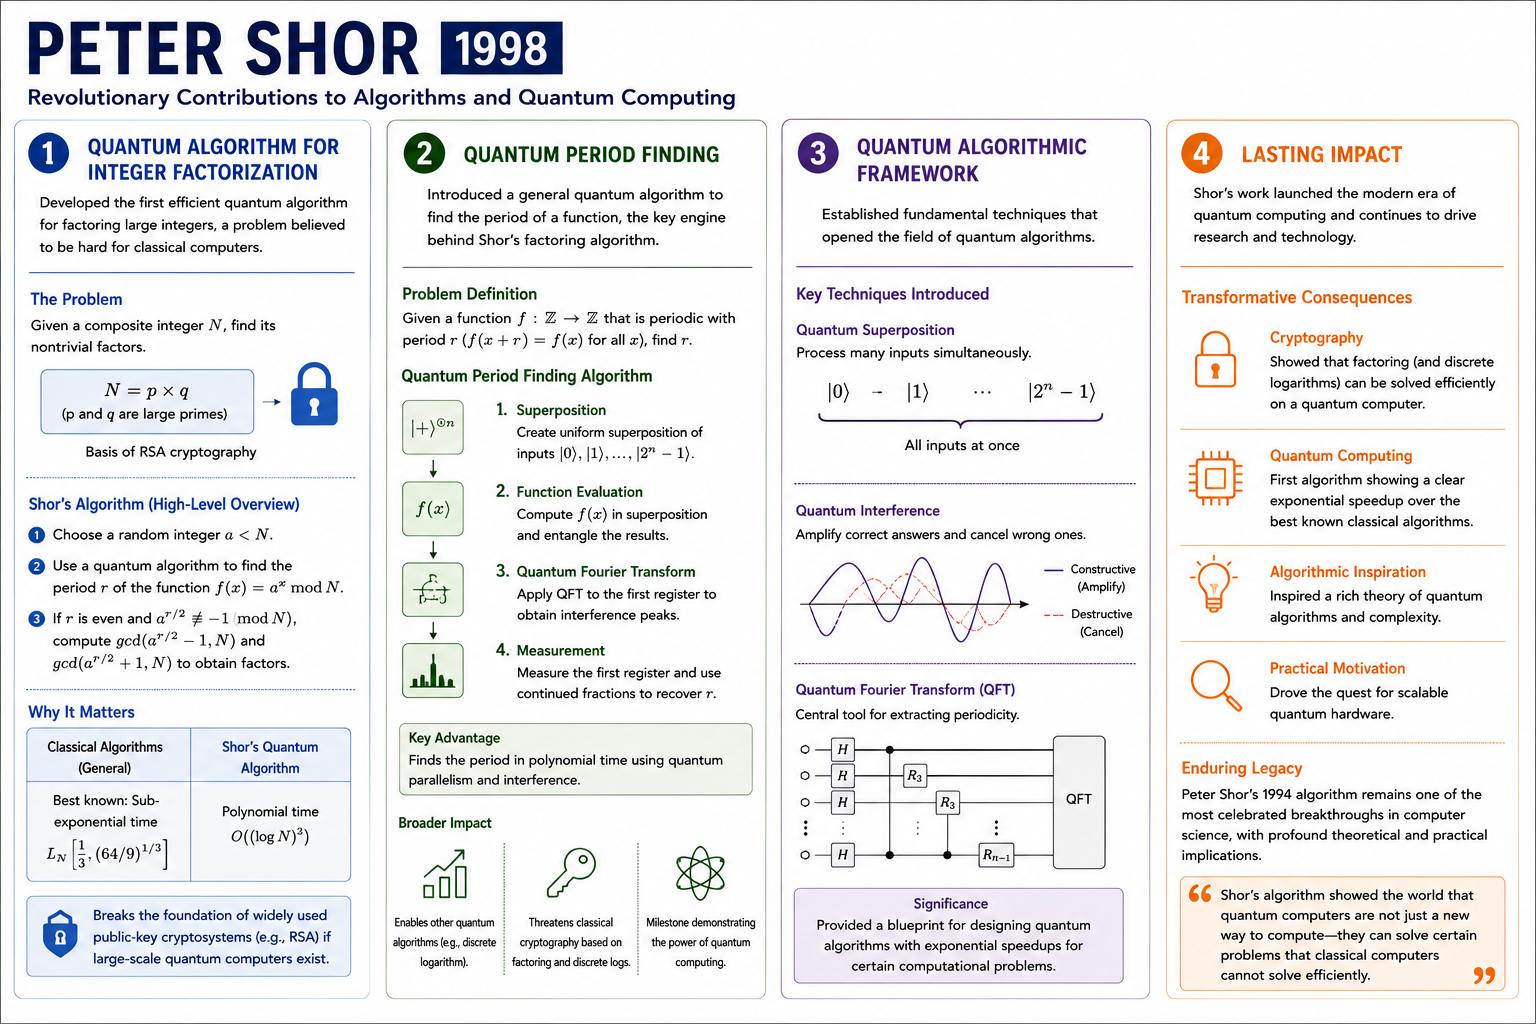
\includegraphics[width=\textwidth]{infographics/abacus5.png}
\end{center}
\targetchapterspacing
\index{Shor, Peter W.}
\booknote{The central habit in this chapter is to hunt for a hidden period, and to ask how interference can make a repeating pattern measurable when sampling one value at a time is too slow.}

\section{An Opening Story: The Wheel and the Strobe Light}

A black wheel with one red dot spins at an unknown rate. Flash a strobe once per second: at the wrong rate the dot darts to a different spot each flash; in time with the wheel it appears frozen. One sample per flash, yet the period is known exactly.

The same trick works when a process repeats every $r$ steps and you may sample it once per step: taken one at a time, the samples look arbitrary. The strobe combines many at once, so combinations agreeing with the true period \emph{add up} and everything else blurs away. Reinforce the compatible, cancel the incompatible---that is the whole mechanism.

In 1998 Peter W. Shor received the Rolf Nevanlinna Prize for building a computer from exactly this mechanism: factoring hides a repeating pattern, and a quantum computer makes it visible and, with the period, obtains the factors.

\section{The Problem}

\noindent\textbf{Factoring.} Multiplying is fast: $23\times 41=943$; reversing it is not. Trial division works for small numbers, but for an $n$-bit $N$, trying all primes up to $\sqrt{N}$ costs about $2^{n/2}$ steps---astronomical at $n=200$. The best classical methods (Pollard's rho, the quadratic sieve, the number field sieve) are still not polynomial: for an $n$-bit input, the number field sieve needs roughly $\exp\!\bigl(c\,n^{1/3}(\log n)^{2/3}\bigr)$ steps. Nobody has proved factoring hard; the belief rests on fifty years of failed attempts.

\noindent\textbf{Why it matters.} Public-key cryptography lives on this asymmetry. In RSA the public key is a product $N=pq$; anyone can encrypt, but only someone knowing $p$ and $q$ can decrypt. The related \emph{discrete logarithm} problem---find $x$ given $g^x\equiv h\pmod p$ for a prime $p$, or the analogous problem on an elliptic curve---protects key exchange and signatures. Both bet that reversing an easy computation is hard.

\noindent\textbf{The physics, in one paragraph.} A qubit is a superposition $\alpha\lvert 0\rangle+\beta\lvert 1\rangle$ with $|\alpha|^2+|\beta|^2=1$; amplitudes can add and cancel, but measuring samples one outcome---0 with probability $|\alpha|^2$---and only that survives. Is there a problem whose difficulty comes from sampling one thing at a time, that a machine built to interfere amplitudes could solve instead?

\section{The World Before}

Factoring grew harder to do as it grew more useful: trial division covers a few digits, Pollard's rho tens of digits, the quadratic sieve reached 100 digits in 1991, and the number field sieve passed 250 digits in the 2020s. All remain subexponential, and RSA keys grew from 512 bits to 2048 because the multiply-versus-factor gap seemed safe.

Quantum computing had a quieter history. Feynman (1982) suggested a quantum machine might be the only efficient way to \emph{simulate} quantum physics; Deutsch (1985) and Deutsch--Jozsa (1992) separated quantum from classical machines only on problems with no practical use. As of the early 1990s no quantum algorithm beat the best classical one on any realistic task, and many doubted a useful quantum algorithm existed.

The doubt was grounded: $n$ qubits represent $2^n$ inputs at once, but measure and you get one random outcome with all structure discarded. \emph{Parallelism alone is not power.} Missing was a way to process amplitudes \emph{before} measuring---letting them add and cancel so a meaningful statistic survives.

\section{The New Idea}

\subsection{Factoring becomes a hidden period}

The pivot is classical number theory: \emph{factoring reduces to finding a period.} Choose $a$ sharing no factor with $N$ (say $a=7$, $N=15$). The powers $a^1,a^2,a^3,\ldots$ modulo $N$ take finitely many values, so they repeat; since $a$ and $N$ share no factor, the first repeated value is $a^1$ itself. The sequence cycles with period $r$, the least positive integer with $a^r\equiv 1\pmod N$, called the \emph{order} of $a$ modulo $N$. Computing powers until the pattern returns---the classical way to find $r$---is the slow, sample-by-sample search the strobe defeats.

What makes $r$ valuable: if $r$ is even and $a^{r/2}\not\equiv -1\pmod N$, then
\[
\gcd(a^{r/2}-1,\,N)\quad\text{and}\quad\gcd(a^{r/2}+1,\,N)
\]
are genuine factors of $N$. Indeed $N$ divides $(a^{r/2}-1)(a^{r/2}+1)$ because it divides $a^r-1$, yet neither factor alone---otherwise the order would be smaller, or $a^{r/2}\equiv-1$---so each gcd pulls out a proper divisor. Finding the factors \emph{is} finding the period.

\subsection{Quantum period-finding: interference does the searching}

Before Shor, a computation was a step-by-step pipeline from input to output. The new idea: compute $a^x\bmod N$ for many $x$ in superposition, then apply an operation that converts \emph{periodic} input into \emph{concentrated} output---the quantum Fourier transform (QFT). A classical Fourier transform already has the strobe's property: a signal of period $r$ concentrates its energy in a few frequencies; a random signal spreads it. The quantum version does this to amplitudes, which can interfere: outcomes agreeing with the hidden period reinforce, others cancel. A measurement then lands, with high probability, on a frequency carrying the period; continued fractions recover $r$, and the number theory above turns it into factors. The speedup is not ``trying every answer at once'': interference moves probability toward answers agreeing with the period and silences the rest.

\subsection{Quantum error correction: protecting the fragile}

A long computation faces a second enemy: the state decays. Classical error correction copies bits and compares---but quantum states cannot be copied, and measuring a qubit collapses it. Shor's solution spreads one \emph{logical} qubit across several \emph{physical} ones and measures carefully chosen combinations whose values reveal which error occurred without revealing the information itself. Redundancy plus a syndrome, arranged so checking does not disturb what it protects. Below a physical error threshold, arbitrarily long computations become possible in principle.

\section{How It Works: Worked Examples}

\subsection{Factoring 15 by order-finding}

Factor $N=15$ by finding the order of $a=7$. First, $\gcd(7,15)=1$. Compute powers modulo 15:
\begin{align*}
7^1&=7,\\
7^2&=49\equiv 4\pmod{15} &&(49-45=4),\\
7^3&=4\cdot 7=28\equiv 13\pmod{15} &&(28-15=13),\\
7^4&=13\cdot 7=91\equiv 1\pmod{15} &&(91-90=1).
\end{align*}
The first power equal to 1 is the fourth, so the order is $r=4$.

Since $r=4$ is even, $a^{r/2}=7^2=49\equiv 4\pmod{15}$, and $4\not\equiv 14\equiv-1\pmod{15}$, so the formula applies:
\[
\gcd(7^2-1,\,15)=\gcd(48,15)=3,\qquad
\gcd(7^2+1,\,15)=\gcd(50,15)=5.
\]
The factors appear directly: $15=3\cdot 5$.

The quantum part supplies $r=4$ without the four-step search: its output is a frequency, and continued fractions recover the denominator 4. The algorithm is probabilistic in two ways: the order may be odd, or $a^{r/2}$ may be $-1$---then the formula fails and one retries with a different $a$; and the measured frequency only approximates a fraction with denominator $r$, so a few runs suffice. The final arithmetic is exact; only the search is probabilistic.

\subsection{A strobe in frequency space: the Fourier transform of a repeating pattern}

Take the length-four signal $[1,0,1,0]$, period 2. Its discrete Fourier transform is $X_k=x_0+x_1\omega^k+x_2\omega^{2k}+x_3\omega^{3k}$, where $\omega=e^{-2\pi i/4}$ is a quarter-turn, so $\omega^2=-1$ and $\omega^4=1$:
\begin{align*}
X_0&=1+0+1+0=2,\\
X_1&=1+1\cdot\omega^2=1-1=0,\\
X_2&=1+1\cdot\omega^4=1+1=2,\\
X_3&=1+1\cdot\omega^6=1-1=0.
\end{align*}
The transform is $(2,0,2,0)$: two peaks, two exact zeros. Repetition has become concentration, exactly as the strobe freezes a wheel; all the mass sits at frequency 0, the constant part, and frequency 2, the rate of repetition.

Contrast the non-repeating signal $[1,1,1,0]$: its transform is $X_0=3$, $X_1=-i$, $X_2=1$, $X_3=i$, magnitudes $(3,1,1,1)$---energy spread across every frequency. In the periodic case the entries agreeing with the repetition add up and the others cancel to zero. The quantum Fourier transform performs this interference on amplitudes, so a single measurement sees the peak and not the noise.

\section{The Mathematics in Brief}

A qubit is a unit vector $\alpha\lvert 0\rangle+\beta\lvert 1\rangle$ with $|\alpha|^2+|\beta|^2=1$; measuring samples 0 or 1 with those probabilities and collapses the state. Several qubits carry $2^n$ coefficients, but an algorithm may touch them only through unitary operations and measurements.

\noindent\textbf{Order.} For $\gcd(a,N)=1$, the \emph{order} $r$ is the least positive integer with $a^r\equiv 1\pmod N$; the sequence $a^x\bmod N$ repeats with period $r$.

\noindent\textbf{The factor-recovery identity.} If $r$ is even and $a^{r/2}\not\equiv -1\pmod N$, then $\gcd(a^{r/2}-1,N)$ and $\gcd(a^{r/2}+1,N)$ are nontrivial factors of $N$. \emph{Why it is true:} $N$ divides $(a^{r/2}-1)(a^{r/2}+1)$ yet divides neither factor, so each gcd lies strictly between 1 and $N$.

\noindent\textbf{The quantum Fourier transform.} A signal of period $r$ has a Fourier transform concentrated at frequencies whose denominators divide $r$. \emph{Why it is true:} values spaced $r$ apart carry identical phase and add; the others spread around the circle and cancel. Shor's algorithm superposes $a^x\bmod N$, applies the QFT, and measures; continued fractions recover $r$ from the measured frequency.

\noindent\textbf{Error correction.} One logical qubit is encoded across many physical qubits, and syndrome measurements reveal errors without revealing the logical state. The threshold theorem: below a physical error rate determined by the code and noise model, arbitrarily long computations become reliable with modest overhead; above it, adding qubits can make things worse.

\noindent\textbf{Where the speed comes from.} The gain is interference, not parallelism: the machine never reads every answer; it arranges amplitudes so answers compatible with the hidden period keep their probability and incompatible answers lose it, then measures once.

\section{Limits and Modern Views}

Current devices remain noisy and far below the fault-tolerant scale required for a cryptographically relevant factorization; the exact physical-qubit count depends on the platform and changes rapidly. Resource estimates commonly place such a computation in the millions of physical qubits. The threshold theorem is a statement about a noise model, not a guarantee about any chip; correlated errors and imperfect operations can violate its assumptions. The theorem, the resource estimate, and the engineering forecast are three different claims; the theory establishes the first, while the third remains open \cite{shor-factoring,shor-error}.

What is threatened, precisely? Systems whose security rests on factoring or discrete logarithms, such as RSA and conventional Diffie--Hellman or elliptic-curve key exchange. Symmetric cryptography (AES, SHA) is different: the best generic quantum attack, Grover's search, only squares the effective security, so doubling the key length restores it. Post-quantum cryptography seeks replacements believed hard even for quantum machines---lattices, error-correcting codes, and hash-based constructions are leading families; isogeny-based proposals remain a research direction after major candidate failures. None is unconditionally safe; each is a bet on an assumption.

\section{Exercises and Self-Study Guide}
\begin{enumerate}[label=\textbf{E\arabic*.}]
\item Verify the factor-recovery formula on another pair: take $N=21$, $a=2$. Compute the powers of 2 modulo 21, find the order, and use the gcd identity to factor 21.
\hint{Follow the 15 example line by line. The order is 6, $2^3=8\not\equiv -1\pmod{21}$, and the two gcds are 7 and 3.}
\item Compute the powers of $a=14$ modulo 15, find its order, and apply the gcd identity. Explain why this $a$ is a poor choice for the algorithm.
\hint{The order is 2 and $a^{r/2}=14\equiv-1\pmod{15}$; the two gcds come out 1 and 15, not proper factors.}
\item Explain why measuring a qubit destroys access to its amplitudes. Give the state $\alpha\lvert 0\rangle+\beta\lvert 1\rangle$ and describe what happens to $\alpha$ and $\beta$ after one measurement.
\hint{After the measurement the state is $\lvert 0\rangle$ or $\lvert 1\rangle$; one amplitude has vanished. Write the probabilities of the two outcomes before the collapse.}
\item Explain why superposition alone is useless, using the coin metaphor: $n$ qubits represent $2^n$ values, yet a measurement returns one random outcome.
\hint{Unless amplitudes were engineered beforehand, the chance that a single sample hits a useful answer is exponentially small.}
\item Compute the discrete Fourier transform of the length-eight signal $[1,0,1,0,1,0,1,0]$ and state where its peaks sit.
\hint{All nonzero entries lie at even positions, so each $X_k$ is a sum of four unit vectors spaced a quarter-turn apart; they add to 4 only at $k=0$ and $k=4$.}
\item List every assumption hidden in a threshold-theorem statement, and identify which one an engineer could measure on a real device.
\hint{Errors are assumed independent or local; gates and measurements must be accurate enough; correction must run fast enough. The effective per-operation error rate is what to measure.}
\item Separate cryptographic primitives into those threatened by order-finding and those affected only by generic quantum search. Justify each placement.
\hint{Order-finding attacks anything built on modular exponentiation, such as RSA and discrete-logarithm key exchange; Grover's search only halves the effective key length of a hash or block cipher.}
\end{enumerate}

\booknote{A final exercise in judgment: before celebrating any quantum speedup, ask what structure the interference is amplifying. If you cannot name the hidden period---the pattern the amplitudes are agreeing on---then the advantage, like the strobe's frozen wheel, may be an illusion of coherence rather than a real discovery.}
\clearpage

\chapter{2002:Madhu Sudan}
\label{chap:sudan}
\begin{center}
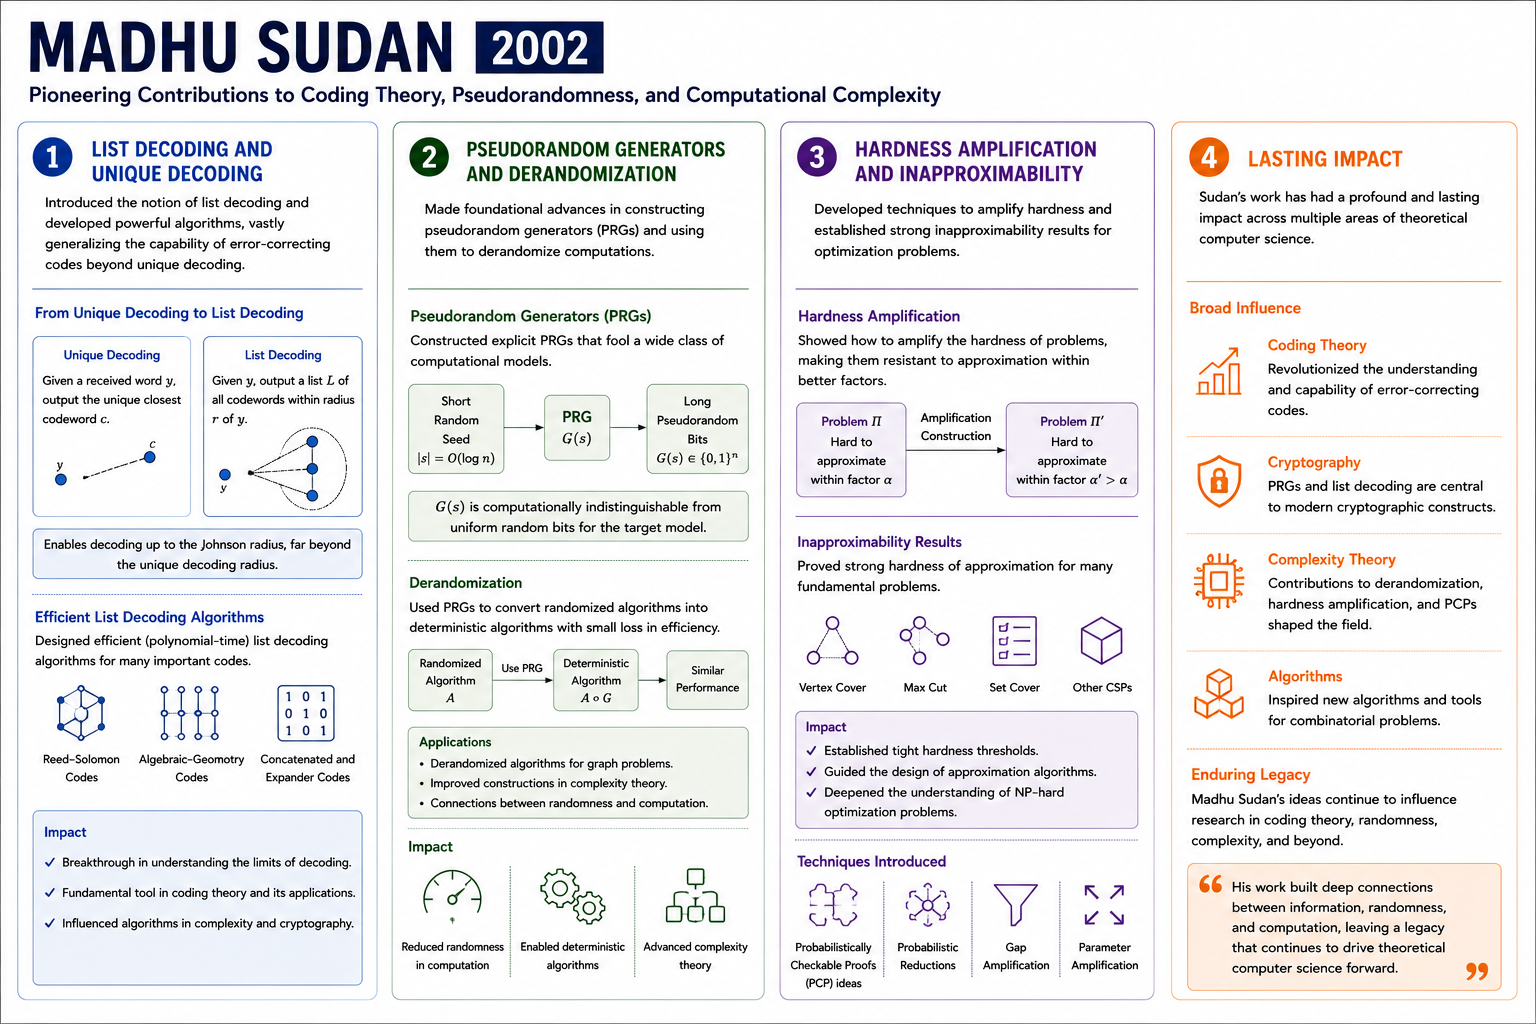
\includegraphics[width=\textwidth]{infographics/abacus6.png}
\end{center}
\targetchapterspacing
\index{Sudan, Madhu}

\booknote{The central habit in this chapter is to treat ambiguity as information: when the noise is heavy, the honest output of a decoder is a short list of every message that could explain what arrived, rather than one forced guess.}

\section{An Opening Story: Two Garbled Words, Four Plausible Messages}

A friend texts you a four-word sentence, and the channel scrambles two of the four words. What arrives is

\emph{MEET ?? OLD ??}

the question marks are unreadable words. The sentence could have been ``MEET AT OLD DOCK,'' ``MEET IN OLD TOWN,'' or ``MEET BY OLD MILL''---each explains exactly the fragments you received. A machine forced to print one sentence must guess---a coin flip that may send you to the wrong place. Two ruined words out of four outrun what cleverness can resolve from this message alone.

Yet the receiver is not helpless: the plausible sentences form a short list, and the true one is on it. A second text---``bring the fishing rod''---narrows the two together to one winner. The first message did not need to decide; it only had to keep every candidate alive until better evidence arrived. That division of labour, \emph{report the ambiguity now, resolve it later}, is the subject of this chapter, and Madhu Sudan's 2002 Rolf Nevanlinna Prize recognized the mathematics that made it efficient.

\section{The Problem}

An error-correcting code expands a message with redundancy so that noise can be repaired. A codeword is a valid expanded message; \emph{decoding} recovers the message from the corrupted string.

The classical contract is strict. If the code has \emph{minimum distance} $D$---the fewest positions in which two codewords differ---a decoder is guaranteed success exactly when the number of corrupted positions is at most $(D-1)/2$: inside that radius the received word is closer to its true codeword than to any other. This is \emph{unique decoding}: one received word, one answer, always right, provided the noise is mild.

Beyond radius $(D-1)/2$ the contract collapses: two codewords can be equidistant from the received word, so no rule always picks the true one. A unique decoder then guesses, and a guess destroys information. The hard question: must decoding stop there, or was the \emph{output contract} wrong?

\section{The World Before}

In 1950 Richard Hamming set the modern framework: a code is a set of strings with minimum distance $D$, and a decoder corrects up to $(D-1)/2$ errors by returning the nearest codeword. Hamming also priced codes---longer codewords buy more protection---so the subject could ask quantitative questions.

Reed--Solomon codes (1960) gave the framework its most beautiful example. Write the message as a polynomial $p(x)$ of degree at most $k$; the codeword is its values $p(a_1),\dots,p(a_n)$ at $n$ fixed points. Two distinct such polynomials agree in at most $k$ positions, so the minimum distance is $D=n-k$. Algebraic algorithms---Berlekamp--Welch, Berlekamp--Massey---decoded these codes in polynomial time all the way to the $(D-1)/2$ bound.

The barrier looked fundamental. A received word can sit halfway between two codewords, so no unique answer is always correct beyond half the minimum distance; this was read as ``heavy noise is hopeless.'' True for unique decoding, false for a different notion of ``the answer.'' In the late 1950s Elias and Wozencraft independently proposed \emph{list decoding}: return every codeword within the radius, not just one. The geometry was clear, but no efficient algorithm existed---trying every message is exponential---so it stayed exotic for thirty-five years.

One well-known fact was the seed: two distinct polynomials of degree at most $k$ agree in at most $k$ points, so agreement is sharp evidence. But organizing the search over all messages without checking them one by one---that nobody saw.

\section{The New Idea}

Sudan's insight begins with a question about what an answer should be. When several messages genuinely explain the received word, returning one candidate is not solving the problem; it hides the fact that the problem has several solutions. The correct output is the set of all explanations. \emph{Ambiguity can be managed mathematically: a short list is a better answer than a forced guess.}

The surprise is that this is not just philosophy; it makes heavy noise tractable. Sudan's 1997 algorithm rests on two counting arguments that expose every plausible message at once.

\emph{Unknowns versus equations.} Seek a nonzero bivariate polynomial $Q(x,y)$ vanishing at every received point $(a_i,b_i)$: one linear equation per point, in $Q$'s unknown coefficients. More coefficients than points means the system is under-determined, so a nonzero solution must exist. Two variables are essential: a univariate $Q(x)$ vanishing at $n$ points needs degree at least $n$, while a bivariate $Q(x,y)$ of small total degree has far more coefficients than $n$.

\emph{Roots versus degree.} If a message $p$ agrees with the received word in $t$ positions, $Q(x,p(x))$ is a univariate polynomial with $t$ roots. When $t$ exceeds its degree, $Q(x,p(x))\equiv0$, so $(y-p(x))$ divides $Q$: \emph{every sufficiently plausible message is a factor of $Q$}. Factoring $Q$ prints the list, which is short: at most one factor per degree of $y$.

Both counts succeed together. Sudan's algorithm then decodes in polynomial time up to roughly $n-\sqrt{2nk}$ errors, and Guruswami--Sudan improves this to roughly $n-\sqrt{n(k-1)}$ under the usual Reed--Solomon conventions; the unique-decoding radius is only about $(n-k)/2$. For small $k$ the list-decoding radii dwarf it, and the only price is a short list. The errors once declared ``impossible'' became routine.

\section{How It Works: Worked Examples}

\subsection{Four symbols, two errors, six honest answers}

Take a Reed--Solomon code with message polynomial $p(x)=2x+1$ of degree $k=1$, evaluated at $x=0,1,2,3$:
\[
(p(0),p(1),p(2),p(3))=(1,3,5,7).
\]
The minimum distance is $D=n-k=3$, so unique decoding corrects at most $(D-1)/2=1$ error. Suppose the received word is
\[
(1,0,0,7),
\]
the second and third symbols (values $3$ and $5$) corrupted. Two errors: unique decoding is beyond its guarantee.

List decoding returns every degree-1 polynomial agreeing with the received word in at least two positions. Since two distinct degree-1 polynomials agree in at most one point, each candidate is identified by the pair of positions where it agrees. From the points $(0,1),(1,0),(2,0),(3,7)$:
\begin{itemize}
\item $(0,1)$ and $(3,7)$: slope $(7-1)/(3-0)=2$, so $p(x)=2x+1$---the true message.
\item $(0,1)$ and $(1,0)$: slope $-1$, so $p(x)=1-x$.
\item $(1,0)$ and $(3,7)$: slope $7/2$, so $p(x)=\frac72(x-1)$.
\end{itemize}
Three more pairs give $p(x)=1-\frac12x$, $p(x)=0$, and $p(x)=7(x-2)$, for six candidates in total.

Check one: $p(0)=1$, $p(1)=0$, matching the received values. Six different messages explain the same evidence, the true one among them. A unique decoder might pick $p=1-x$ and lose the message; the list keeps $2x+1$ alive until later evidence selects it. (Reals are used for familiar arithmetic; over any field with at least four evaluation points the story is identical.)

\subsection{The bivariate polynomial in action}

Now use Sudan's machinery on the same points $(0,1),(1,0),(2,0),(3,7)$. A bivariate polynomial of total degree at most $2$ has $6$ coefficients:
\[
Q(x,y)=c_0+c_1x+c_2y+c_3x^2+c_4xy+c_5y^2.
\]
Requiring $Q(a_i,b_i)=0$ at the four points gives four homogeneous linear equations in six unknowns, so a nonzero solution must exist. One is
\[
Q(x,y)=7x^2+2y^2-21x-16y+14.
\]
Check: at $(0,1)$, $0+2-0-16+14=0$; at $(1,0)$, $7+0-21+0+14=0$; the other two cancel the same way. \emph{More unknown coefficients than constraints forces a nonzero $Q$}, and finding it is routine linear algebra.

Now substitute a candidate. For the true message $p=2x+1$,
\[
Q(x,2x+1)=15x^2-45x=15x(x-3),
\]
with roots $x=0,3$, exactly its agreement positions. For $p=1-x$,
\[
Q(x,1-x)=9x^2-9x=9x(x-1),
\]
roots at $x=0,1$. Here agreement $t=2$ equals the degree of $Q(x,p(x))$, so roots appear but are not forced; the forcing step needs the counting tilted. In Sudan's real regime---many points, $k\ll n$---a genuine candidate agrees in $t$ positions \emph{exceeding} that small degree; $Q(x,p(x))$ then has more roots than its degree permits, vanishes identically, and the candidate is a factor of $Q$. Factoring $Q$, or solving for its $y$-roots, prints the whole list in polynomial time.

\section{The Mathematics in Brief}

\emph{The agreement lemma.} Two distinct polynomials of degree at most $k$ agree in at most $k$ points. Why: their difference is a nonzero polynomial of degree at most $k$, which has at most $k$ roots.

\emph{Reed--Solomon geometry.} A message is a polynomial of degree at most $k$; its codeword is its $n$ values. Hence $D=n-k$ and the unique radius is $(D-1)/2=(n-k-1)/2$.

\emph{The list-decoding radius.} A Johnson-type bound says that for any code of distance $D=n-k$, agreement radius $\sqrt{nk}$ (about $n-\sqrt{nk}$ errors) yields only a polynomially bounded list. Sudan achieves this up to a constant factor ($n-2\sqrt{nk}$); Guruswami--Sudan reaches the Johnson bound exactly. The formula $\sqrt{nk}$ balances the counting: enough points for a sparse $Q$, yet enough agreements for $t$ to outrun the degree of $Q(x,p(x))$.

\emph{The $Q(x,y)$ method.} Choose $Q$ with more coefficients than points, so $Q(a_i,b_i)=0$ has a nonzero solution. A candidate agreeing in $t$ positions makes $Q(x,p(x))$ a degree-$(<t)$ polynomial with $t$ roots; it must vanish identically, so $p$ divides $Q$. With $B$ bounding the $y$-degree, the list has at most $B$ members. Every inequality has an algorithmic meaning: existence from linear algebra, extraction from factoring.

\emph{The proof-checking connection.} The same ``local evidence forces a global conclusion'' pattern powers probabilistically checkable proofs: encode a long proof, test a local relation at a few random positions, and let distance make a wrong proof fail most tests. Decoding and proof-checking are two faces of one idea: \emph{redundancy turns a few observations into a guarantee about the whole object}.

\section{Limits and Modern Views}

The list is polynomially bounded but not free: its precise size depends on the radius and interpolation parameters, and the field must supply $n$ distinct evaluation points, limiting block length; algebraic-geometry codes relax this and give the best known length--rate--distance tradeoffs. The Guruswami--Sudan refinement---weights and multiplicities in the interpolation---reaches the Johnson bound and extends to \emph{soft-decision decoding}, where each symbol carries a reliability score and weights favour trustworthy positions.

The PCP connection went beyond metaphor. These algebraic verification ideas became the engine of the PCP theorem---every proof can be encoded so that a verifier reading a constant number of random positions separates valid proofs from almost all invalid ones---and from it came hardness of approximation: problems like MAX-3SAT are hard even to approximate \cite{sudan-list,sudan-pcp}. Engineering inherited the same ideas: erasure coding (Reed--Solomon's descendant) protects RAID arrays and data centres, and list decoding appears in regenerating codes that repair a failed node from a few surviving blocks.

List decoding remains the honest statement of what decoding means. Heavy noise is not ``unsolvable''; it produces a short list, and shortening it to a winner is a job for side information, not the decoder. The field's slogan changed from ``correct the errors'' to ``know the plausible messages.''

\section{Exercises and Self-Study Guide}
\begin{enumerate}[label=\textbf{E\arabic*.}]
\item Prove the agreement lemma: two distinct polynomials of degree at most $k$ agree in at most $k$ points.
\hint{Subtract the two polynomials; a nonzero polynomial of degree at most $k$ has at most $k$ roots.}

\item Verify that $(1,0,0,7)$ is at Hamming distance $2$ from the codewords of both $p=2x+1$ and $p=1-x$, while the unique-decoding radius is $1$. Why must a unique decoder guess?
\hint{Write both codewords and count differing positions; a distance-$3$ code cannot tell them apart at radius $2$.}

\item Set up $Q(x,y)=c_0+c_1x+c_2y+c_3xy$ vanishing at the four received points and show it has only the zero solution; explain why adding $x^2$ and $y^2$ terms yields a nonzero one.
\hint{The first three points force $c_0=c_1=c_2=0$, the fourth forces $c_3=0$: four unknowns, four equations, no slack.}

\item A Reed--Solomon code has $n=100$ points and message degree $k=5$. Compare the unique-decoding radius with the list-decoding radius and state the agreement threshold for a guaranteed place on the list.
\hint{Unique radius $(n-k-1)/2\approx47$; list radius about $100-\sqrt{500}\approx78$ errors; the Johnson threshold is roughly $t>\sqrt{nk}\approx22$.}

\item Explain why $Q$ must have two variables; what goes wrong with a univariate $Q(x)$?
\hint{To vanish at $n$ points a univariate $Q$ needs degree at least $n$, so coefficients never beat the equations; the second variable carries the received value.}

\item The repetition code maps $0\mapsto000$, $1\mapsto111$. A local test reads two random positions and accepts if they match. Show it never rejects a valid codeword, and compute the rejection probability for $001$.
\hint{For $001$ the pairs $(0,0),(0,1),(0,1)$ disagree in two of three cases.}

\item Give an example where the worked-example list collapses to one message only after a second constraint, and name the constraint.
\hint{The received word cannot separate $2x+1$ from $1-x$; a second transmission revealing $p(1)=3$ leaves only $2x+1$.}
\end{enumerate}

\booknote{A final exercise in judgment: whenever a decoder is forced to return one answer, ask whether the ambiguity it suppresses is real. If two messages genuinely explain the same evidence, the honest output is the list; the winner should be chosen by side information, not by the decoder.}
\clearpage

\chapter{2006:Jon Kleinberg}
\label{chap:kleinberg}
\begin{center}
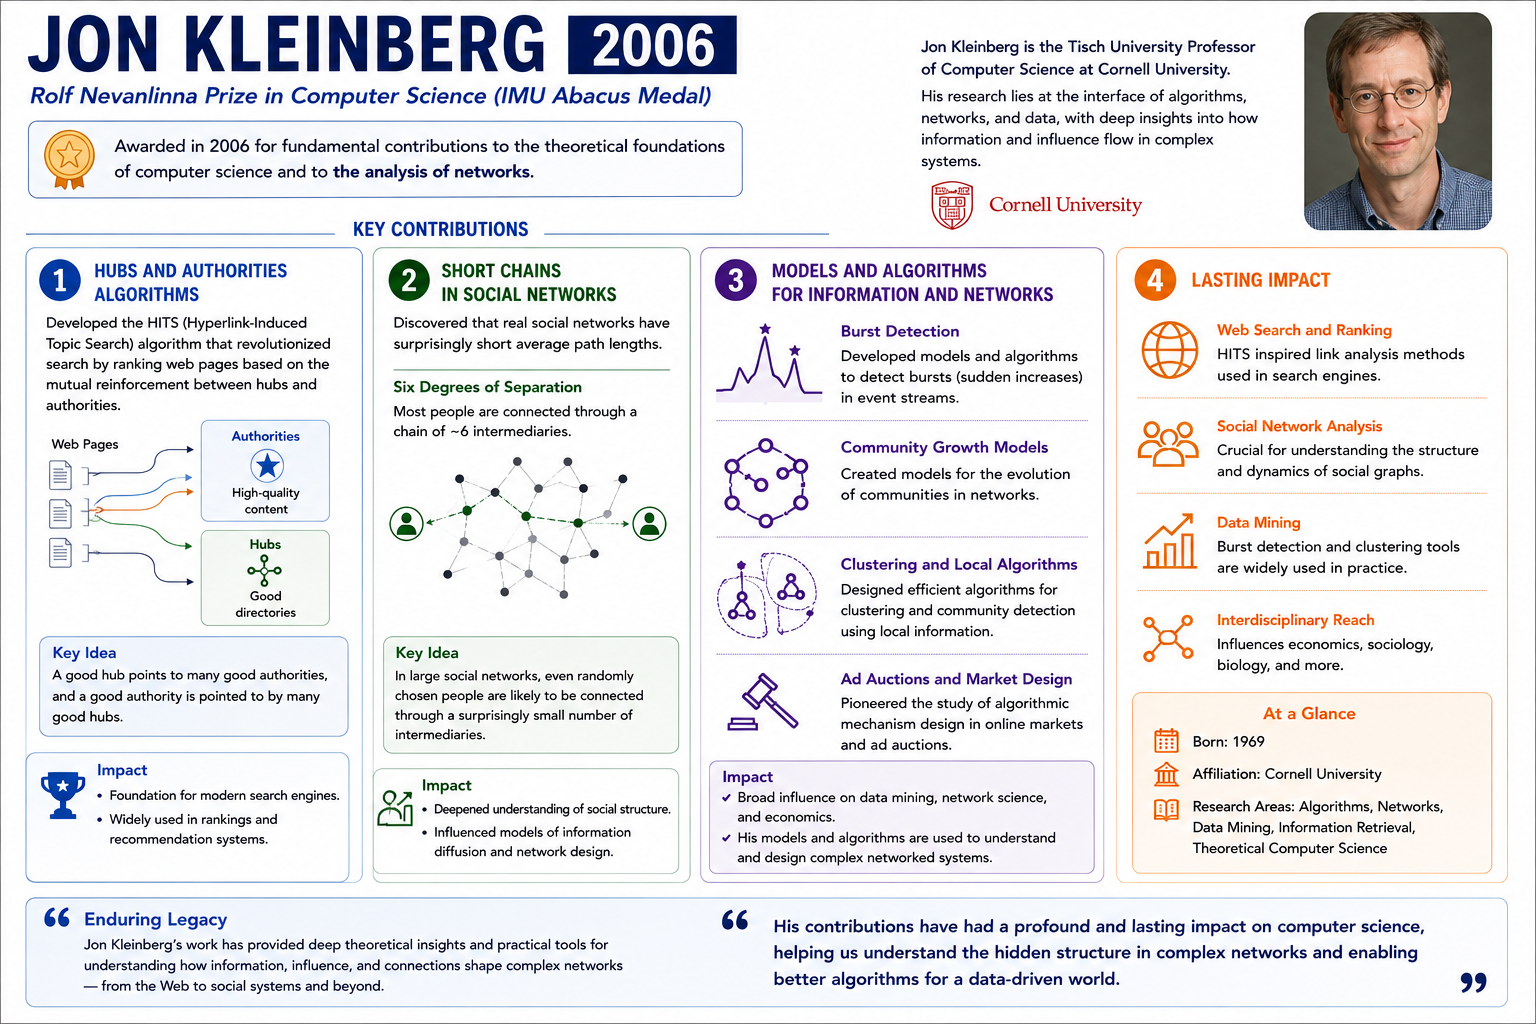
\includegraphics[width=\textwidth]{infographics/abacus7.png}
\end{center}
\targetchapterspacing
\index{Kleinberg, Jon}
\booknote{The central habit in this chapter is to state what local information an algorithm may use and what global question it must answer---and then to name the reinforcement rule whose equilibrium the answer represents.}

\section{An Opening Story: A Recipe Site Where Popularity Is Circular}
Maya runs a small cooking site with four pages. Page A holds a famous lasagna recipe; page B, a weeknight-dinner blog, links to A; page C, a family recipe box, links to B and A; page D, a kitchen forum, links to C. Nobody links to D.

Which page answers ``lasagna''? Count incoming links: A has two, B and C have one, D has none. Ask which is most \emph{trusted} and the reasoning turns circular: A is trusted because good pages point to it, B because C points to it, C because D points to it, D because \ldots nothing. Popularity defined by popularity has no answer until we agree on a rule that breaks the circle.

\section{The Problem}
Network data arrives locally: a search engine sees millions of pages and the links among them; a person reaching a stranger sees only their own friends; a log shows one event at a time. Yet the questions worth asking are global: which pages are authoritative? Can someone reach a distant person using only nearby contacts? Is an hour of frantic activity a real story or ordinary noise?

A single local observation carries almost no information; the answer lives in the whole pattern. The difficulty is \emph{aggregation}. Three problems make this concrete:
\begin{itemize}
\item \textbf{Ranking.} Given the web's links, rank pages so authoritative ones rise to the top.
\item \textbf{Navigation.} Given a network with long-range shortcuts, reach a distant target using only local information.
\item \textbf{Burst detection.} Given a stream of timestamped events, decide when the rate genuinely rises and where bursts begin and end.
\end{itemize}
Each is easy to state and easy to get wrong: ranking is gameable, navigation can be blocked by information never seen, and bursts hide inside random variation.

\section{The World Before}
Early search engines matched query words against page text. Simple---and a standing invitation to cheat: a page repeating ``lasagna recipe'' twenty times outranked a better page using the phrase once. Keyword-stuffed pages became the norm; raw text was trivial to game.

Counting incoming links was the natural fix: more pages pointing at you meant more people found you useful. Harder to fake with one page, but not with a thousand---a \emph{link farm} is a cluster of pages built only to point at one target. Counting also hid the circularity of the recipe puzzle: a page is popular partly because \emph{popular} pages link to it.

Social networks had a folklore theorem: Milgram's letter experiments suggested a small diameter, about six handoffs between any two people, so navigation must be easy. But a person can only hand a letter to someone they know. Small diameter says a short path \emph{exists}; it says nothing about whether someone who sees only their own acquaintances can \emph{find} it. The inference---short paths imply easy navigation---is not merely unproven; it is false.

Bursts had a statistical description, but no algorithm for finding where a rate changes; eleven messages in ten minutes could be a burst or ordinary luck. Two ideas were missing: an \emph{explicit model of mutual reinforcement}, turning circular importance into a computable fixed point, and an \emph{explicit model of the information a local navigator has}, separating ``a short path exists'' from ``a local rule can find it.'' Kleinberg's 2006 Nevanlinna Prize recognized precise answers to all three.

\section{The New Idea}
\subsection{HITS: two roles, one fixed point}
An \emph{authority} is worth reading; a \emph{hub} is worth following. They reinforce each other: good authorities are linked by good hubs, and good hubs link to good authorities.

Break the circle by iteration. Start every score at $1$, then alternate:
\begin{itemize}
\item \textbf{Authority update:} new authority $=$ sum of the hub scores of the pages linking to it.
\item \textbf{Hub update:} new hub $=$ sum of the authority scores of the pages it links to.
\end{itemize}
Rescale after each round. The mutual definition becomes concrete arithmetic that settles down. In matrix language,
\[
a\leftarrow A^{\mathsf T}h,\qquad h\leftarrow Aa,
\]
and the stable scores are the principal singular vectors of the adjacency matrix $A$.

\subsection{The small-world model: what a local navigator can use}
Lay the network on a two-dimensional grid. Each person knows their grid neighbors and a few \emph{shortcuts}---long-range contacts. The navigator's rule is greedy and myopic: move to the contact closest to the target; no one sees the map.

Suppose node $u$ links to node $v$ with probability proportional to $d(u,v)^{-r}$. The answer is sharp:
\begin{itemize}
\item $r=2$: polylog expected steps;
\item $r<2$: too-uniform shortcuts---polynomial time;
\item $r>2$: too-local shortcuts---polynomial time.
\end{itemize}
The $2$ is the grid's dimension. From distance $\delta$ to the target, the useful jumps land in the \emph{halving ball}---nodes within $\delta/2$ of the target---about $\delta^{2}$ of them, each reached with probability about $1/\delta^{2}$. A useful jump has comparable probability at every scale, so $\log_2 n$ halvings reach the target.

\subsection{Bursts: separating a baseline from a self-exciting process}
A burst is a stretch in which events arrive faster than the baseline rate. Kleinberg's model uses hidden states: a normal state at rate $\lambda_0$ and a burst state at rate $\lambda_1>\lambda_0$. Assigning each event to a state while explaining the observed waiting times and paying a penalty per switch turns a burst into an \emph{inferred hidden structure} rather than a claim that each event directly causes the next.

\subsection{The conceptual shift}
All three models make explicit what information the algorithm may use and what rule converts it into an answer. The conclusions are precise and surprising: \emph{local connectivity can generate useful global signals, but only when the definition of relevance is explicit; and small diameter does not imply navigability.}

\section{How It Works: Worked Examples}
\subsection{Example 1: HITS by hand on four pages}
Maya's site as a directed graph: $B\to A$, $C\to A$, $C\to B$, $D\to C$. Start all scores at $1$.

Round 1, authority ($a_j=$ sum of hub scores of pages linking to $j$):
\[
a_A=h_B+h_C=2,\qquad a_B=h_C=1,\qquad a_C=h_D=1,\qquad a_D=0.
\]
Round 1, hub ($h_i=$ sum of authority scores of pages $i$ links to):
\[
h_A=0,\qquad h_B=a_A=2,\qquad h_C=a_A+a_B=3,\qquad h_D=a_C=1.
\]
Round 2, authority:
\[
a_A=h_B+h_C=2+3=5,\qquad a_B=h_C=3,\qquad a_C=h_D=1,\qquad a_D=0.
\]
Round 2, hub:
\[
h_A=0,\qquad h_B=a_A=5,\qquad h_C=a_A+a_B=5+3=8,\qquad h_D=a_C=1.
\]
Collect the two rounds: authority $(2,1,1,0)\to(5,3,1,0)$, hub $(0,2,3,1)\to(0,5,8,1)$. A rises as the dominant authority, C as the dominant hub. Renormalizing after each round---dividing by the length of each score vector---keeps the iteration convergent without changing which page is largest. These scores are the \emph{equilibrium of this rule}, not an objective fact about the pages.

\subsection{Example 2: greedy routing on a 4 by 4 grid}
Draw a $4\times4$ grid, target at $(4,4)$, navigator at $(1,1)$; without shortcuts the trip takes $6$ steps.

Give $(1,1)$ a shortcut to $(3,3)$. Greedy compares options: $(1,2)$ is $5$ from the target, $(2,1)$ is $5$, the shortcut endpoint is $2$. It jumps, then $(3,3)\to(3,4)\to(4,4)$: three steps, and the jump cut the remaining distance from $6$ to $2$---roughly in half.

How should shortcuts be distributed? From the corner $(1,1)$ the grid has two nodes at distance $1$, three at $2$, four at $3$, three at $4$, two at $5$, one at $6$. Under $r=2$ (probability proportional to $1/d^2$):
\begin{center}
\begin{tabular}{lcccccc}
\toprule
distance $d$ & 1 & 2 & 3 & 4 & 5 & 6 \\
\midrule
chance & $57\%$ & $21\%$ & $13\%$ & $5\%$ & $2\%$ & $0.8\%$ \\
\bottomrule
\end{tabular}
\end{center}
Short jumps dominate; under a uniform law ($r=0$) every distance is equally likely at about $6.7\%$, so no scale can be counted on. The contrast is decisive at scale $n$: the halving ball holds about $\delta^{2}$ nodes, each reached with probability about $1/\delta^{2}$, so a useful jump has comparable chance at every scale and $\log_2 n$ halvings reach the target. Under $r<2$ the longest links dominate and the halving chance collapses; under $r>2$ shortcuts almost never reach half the gap. Both force polynomial time.

\section{The Mathematics in Brief}
\textbf{HITS.} The iteration
\[
a\leftarrow A^{\mathsf T}h,\qquad h\leftarrow Aa
\]
with normalization is power iteration for the symmetric matrices $A^{\mathsf T}A$ and $AA^{\mathsf T}$, converging to the principal singular-vector pair of $A$. \emph{Why:} substituting gives $a\leftarrow A^{\mathsf T}Aa$, and repeated multiplication by a symmetric matrix amplifies the largest-eigenvalue direction while shrinking all others.

\textbf{Small-world navigation.} Shortcuts follow
\[
\PP(u\text{ links to }v)\propto d(u,v)^{-r}.
\]
On an $n\times n$ grid, greedy routing takes $O((\log n)^2)$ expected steps when $r=2$ and $\Omega(n^{\beta})$ for a constant $\beta>0$ when $r\ne2$. \emph{Why:} under $r=2$ the normalization sum is $\Theta(\log n)$, so the halving ball is hit with probability $\Theta(1/\log n)$ per shortcut; under $r<2$ the halving chance is $\Theta((\delta/n)^{2-r})$; under $r>2$ shortcuts never reach the ball. The exponent must equal the dimension.

\textbf{Bursts.} Waiting times are exponential at rate $\lambda_0$ in the normal state and $\lambda_1>\lambda_0$ in the burst state; the model picks the assignment of events to states that best explains the observed waits, minus a penalty per switch. \emph{Why:} a constant-rate model predicts long runs of very short waits to be exponentially unlikely, so when they occur a state switch is the parsimonious explanation; the penalty stops a new burst being declared around every event.

\textbf{The distinction.} A centralized algorithm knows the whole graph; a navigator sees only its position and contacts. ``There is a short path'' and ``a local rule can find it'' are different statements, and the small-world theorem draws the line between them.

\section{Limits and Modern Views}
The HITS equilibrium is not a neutral measure. A tightly connected community can dominate without being globally authoritative, and a feedback loop can lock in an early accident: top-ranked pages attract attention, attention creates links, links raise the rank \cite{kleinberg-hits}. A link is not a causal statement: two pages may link because they share an audience, a platform may recommend both, and friendship and purchase may share a hidden cause. Rankings amplify these hidden causes, so modern work asks causal questions alongside graph questions \cite{kleinberg-smallworld}.

Models are static while networks move, so a static eigenvector lags the system it summarizes; popularity attracts links partly because it is already popularity. Strategic actors game whatever signal is scored---link farms, coordinated bots, engineered cascades---so the evidence is adversarial \cite{kleinberg-bursts}. Rankings encode past inequalities, attention measurements touch privacy, and an engagement-optimal ranking can worsen the decision it supports; fairness-aware and privacy-preserving models now share the agenda.

Kleinberg's style survives these harder questions: name the mechanism, derive a testable prediction, then check which parts survive contact with data. The model is a hypothesis to test, not reality itself.

\section{Exercises and Self-Study Guide}
\begin{enumerate}[label=\textbf{E\arabic*.}]
\item Run one more HITS round on the worked example from $a=(5,3,1,0)$, $h=(0,5,8,1)$. Confirm $A$ stays the top authority and $C$ the top hub.
\hint{Authority of a page is the sum of the hub scores of pages linking to it; hub is the sum of the authority scores of the pages it links to.}
\item On the three-page graph $A\to B$, $A\to C$, $B\to C$, compute two HITS rounds from all-ones scores. Which page becomes the top authority, and which the top hub?
\hint{$a_A=0$ because nothing links to $A$; $C$'s authority and $A$'s hub score grow fastest.}
\item On a $3\times3$ grid, place a shortcut from $(2,2)$ to $(1,1)$ and run greedy routing to target $(1,1)$ from $(2,2)$ and from $(1,3)$. When does the shortcut help, and when is it invisible?
\hint{Greedy moves to the contact closest to the target; a shortcut is usable only from its source node.}
\item Two streams of twenty events each: $S$ has one event every 100 minutes; $T$ has nineteen events in the first 90 minutes, then silence. Same average rate. Which is a burst, and how does a model detect it?
\hint{Compare inter-arrival times: $S$ has waits near 100 minutes, $T$ has many tiny waits followed by one huge one.}
\item Describe a confounding variable that could make friendship links look as though they cause purchases.
\hint{A shared experience---a new TV show, a holiday, a company policy---can create both the friendship and the purchase.}
\item Remove the link $D\to C$ and rerun HITS for two rounds. Does $A$ remain the top authority? Propose a simple stability test for a ranking when links change.
\hint{Rerun with the link deleted and compare the ordering of the top pages before and after.}
\item On the $4\times4$ grid, put a shortcut from $(1,2)$ to $(4,4)$ and route from $(1,1)$ to $(4,4)$. With full knowledge the shortest path is $(1,1)\to(1,2)\to(4,4)$: two steps. Simulate greedy, breaking ties toward the larger row number. How many steps, and why does it miss the shortcut?
\hint{Greedy sees a shortcut only when standing at its source; the tie-break at $(1,1)$ decides whether the walk ever reaches $(1,2)$.}
\end{enumerate}

\booknote{A final exercise in judgment: whenever a ranking is published or a path is followed, name the reinforcement rule that produced the score and the local information the navigator was allowed to see. A number that cannot be traced to a stated rule is not a finding; it is a guess wearing notation.}
\clearpage

\chapter{2010:Daniel Spielman}
\label{chap:spielman}
\begin{center}
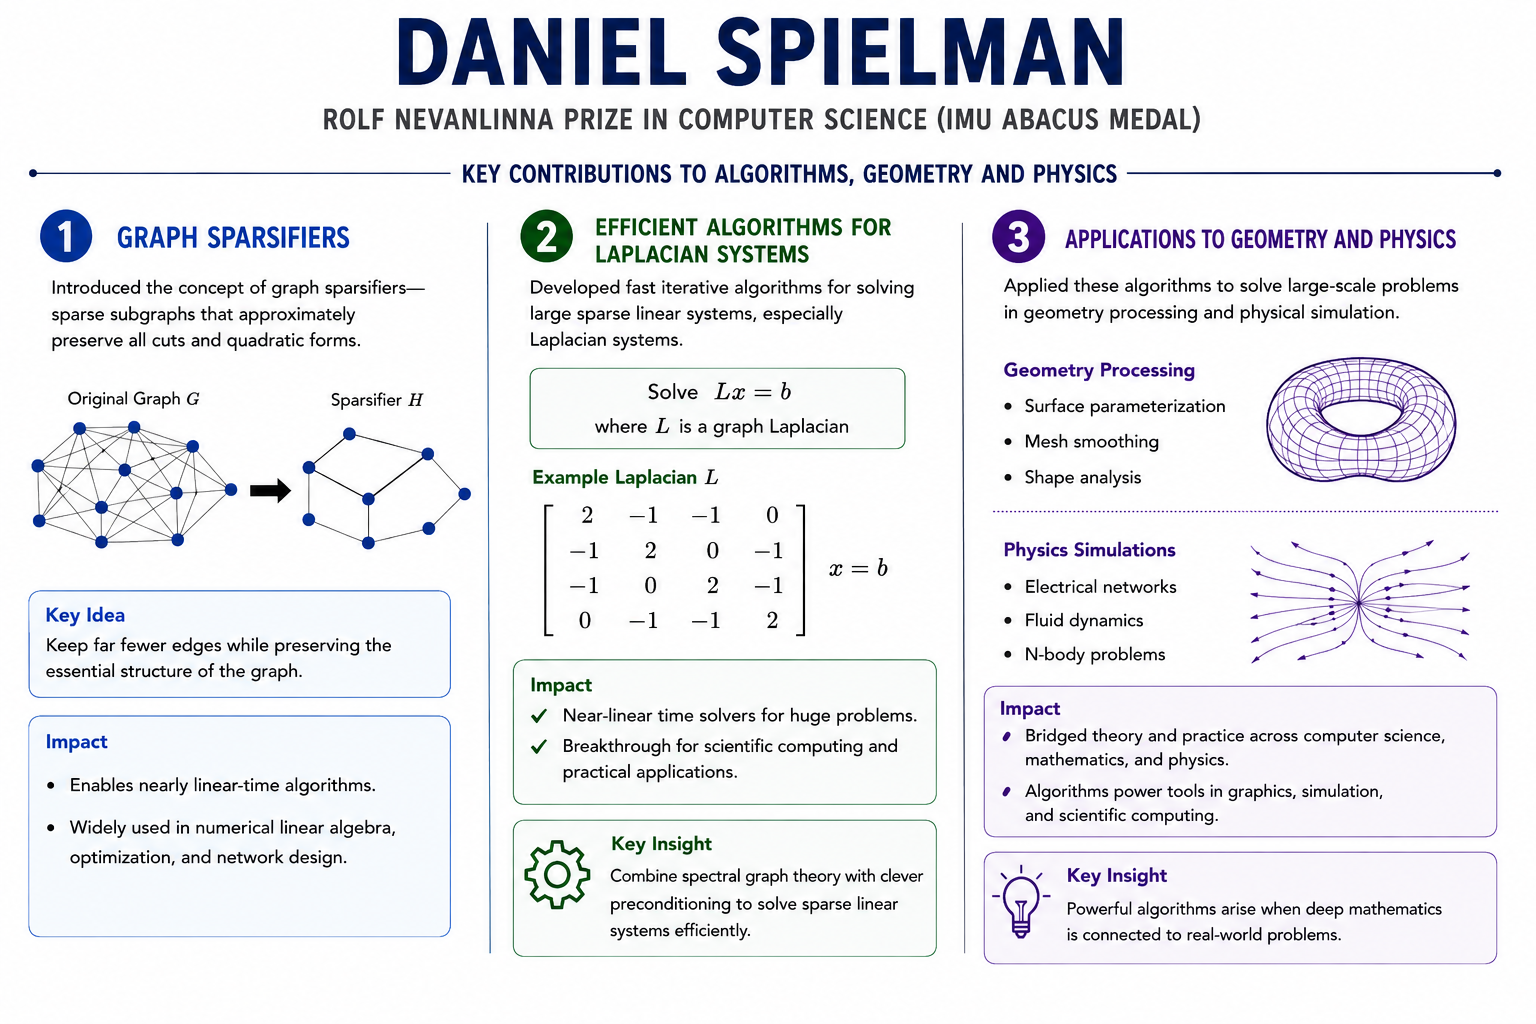
\includegraphics[width=\textwidth]{infographics/abacus8.png}
\end{center}
\targetchapterspacing
\index{Spielman, Daniel}
\booknote{The central habit in this chapter is to translate a network into a matrix and to demand of every approximation one thing: it must preserve the energy geometry of the original graph.}

\section{An Opening Story: Springs on a Water Line}

Three buildings stand in a row, each pair of neighbours joined by a pipe. Pipes resist differences: neighbours with pressures $u$ and $v$ stretch a pipe by $(u-v)^2$. For pressures $2$, $0$, $-1$, the pipes stretch by $(2-0)^2=4$ and $(0-(-1))^2=1$, total tension $5$: every assignment of pressures carries one number, the network's total tension.

Two questions seem far apart. \emph{Where is the weak joint?} A strong cluster meeting another across one rusty pipe lets pressures change on either side while tension stays small---the network is nearly two pieces. \emph{What pressures does the network settle at?} One linked equation per building; for a city, a huge system. Daniel Spielman's 2010 Rolf Nevanlinna Prize recognized that both are the same information read two ways, and that a matrix is the bookkeeping making the connection visible.

\section{The Problem}
Three problems about big networks, all questions a computer must answer quickly.

\noindent\textbf{Solving huge sparse systems.} Physical simulations produce one equation per point, coupling each point to its neighbours. A million-point mesh gives $Lx=b$ with a million unknowns and a handful of nonzeros per row; solving it directly is far too slow.

\noindent\textbf{Finding weak cuts.} Divide a network into two parts so little flows between them: communities, power-grid islands, circuit halves. The question is global---a weak cut is felt across the network, not at one edge---so examining edges one at a time answers nothing.

\noindent\textbf{Explaining practical speed.} The simplex method is excellent in practice yet has an astronomically slow worst case. Both are true; nobody could explain how.

Each was stuck because nobody could read a network's global behaviour, and because worst-case analysis ignored the noise in real inputs.

\section{The World Before}

Gaussian elimination costs about $n^3/3$ operations and destroys sparsity: a $1000\times1000$ grid yields a matrix with a million rows and about five million nonzeros, which elimination fills to roughly $10^{12}$ entries. So huge sparse systems were attacked with iterative methods---conjugate gradients, multigrid---which keep the matrix sparse and, in practice, converged quickly. Provable guarantees were far weaker than observed behaviour, and the fastest methods needed special geometry.

Graph partitioning used flows and heuristics. Finding a minimum cut by max-flow is correct but expensive, and heuristic searches had no guarantee. No one had a theorem saying: this linear-system solution cuts the graph into provably good pieces.

Linear programming was the most embarrassing case. Klee and Minty built a small cube on which the simplex method visits an exponential number of corners---a formal disaster---yet practitioners ran it daily and loved it. Worst-case analysis had no vocabulary for the difference.

Two ingredients were missing: a translation of a discrete graph into a matrix recording its bottlenecks, currents, and mixing faithfully; and an analysis that respects reality---real inputs carry noise, so a proof should be able to call a pathological input fragile.

\section{The New Idea}
Stop looking at one edge at a time. Write the network as a matrix, define an energy on assignments, and let the matrix's eigenvalues---numbers attached to the whole network---carry the answers.

\subsection{The Laplacian: springs as bookkeeping}
Build $L$ with off-diagonal entry $-w_{ij}$ for the edge joining $i$ and $j$ and diagonal entry the sum of the weights meeting $i$: $L=D-A$, degree matrix minus adjacency, the \emph{graph Laplacian}. For an assignment $x$,
\[
x^{\mathsf T}Lx=\sum_{(i,j)}w_{ij}(x_i-x_j)^2,
\]
the opening story's tension: the matrix turns every assignment into an energy.

Which assignments carry little energy for their size? Two dense parts joined by a thin thread admit $+1$ on one part, $-1$ on the other, differing only across the thread. The Rayleigh quotient $x^{\mathsf T}Lx/x^{\mathsf T}x$ measures this ratio; its minimum is the smallest eigenvalue, always $0$ (the constant assignment). The \emph{second-smallest} eigenvalue $\lambda_2$ is small exactly when the graph can be cut cheaply, and its eigenvector rounds into a provably good partition. Cheeger-type inequalities quantify this: the graph's expansion $h$ is sandwiched between a constant multiple of $\lambda_2$ and roughly its square root.

\subsection{Spectral sparsification: a small graph with the same energy}
A spectral sparsifier replaces the graph by a weighted graph with far fewer edges preserving every quadratic form within $(1\pm\eps)$:
\[
(1-\eps)x^{\mathsf T}Lx\leq x^{\mathsf T}\widetilde Lx\leq(1+\eps)x^{\mathsf T}Lx\quad\text{for all }x.
\]
``For all $x$'' is the honesty condition: the small graph imitates the large one on every assignment, so every computation on it is valid for the large one.

\subsection{Recursive preconditioning: nearly-linear solvers}
The energy view also speeds up solving $Lx=b$. An iterative solver converges in steps controlled by the spread of eigenvalues, and a \emph{preconditioner}---a change of coordinates balancing scales---shrinks that spread. Spielman and Teng built it from the graph: a hierarchy of sparsifiers, each level sparse and guaranteeing the next. Result: Laplacian systems solved in nearly linear time, order $m\log^{O(1)}n$.

\subsection{Smoothed analysis: the fragility of worst cases}
The fourth idea concerns the simplex method. Under a specified perturbation model and a specified pivot rule, let an adversary choose the input and then add small random noise to the coefficients. Degenerate configurations---corners where many constraints meet exactly---are typically destroyed, and Spielman and Teng proved polynomial expected running time for their smoothed-analysis setting. Worst cases still exist; the theorem says that the analyzed perturbations make them statistically fragile.

The shift is two-sided: a discrete problem can be translated into linear algebra without losing the structure that matters---bottlenecks become small eigenvalues, cuts become eigenvectors, flows become voltages---and worst cases can be fragile.

\section{How It Works: Worked Examples}
\subsection{A path of three springs}
Three vertices $1,2,3$ in a line, every edge of weight $1$:
\[
L=\begin{pmatrix}1&-1&0\\-1&2&-1\\0&-1&1\end{pmatrix}.
\]
For $x=(1,0,-1)$, the edges stretch by $(1-0)^2=1$ and $(0-(-1))^2=1$, so $x^{\mathsf T}Lx=2$. Multiplying by $L$ gives $L(1,1,1)=(0,0,0)$, $L(1,0,-1)=(1,0,-1)$, $L(1,-2,1)=3(1,-2,1)$, so the eigenvalues are $0,1,3$. The small eigenvalue $1$ says the path splits for the price of one edge; its eigenvector $(1,0,-1)$ points at the cut $\{1\}$ versus $\{2,3\}$.

\subsection{Two tight clusters, one weak thread}
Two tight pairs, $1,2$ and $3,4$, each joined by weight $10$, plus a weak thread of weight $0.1$ joining $2$ to $3$. With $x=(1,1,-1,-1)$, the internal springs stretch nothing and only the thread stretches:
\[
x^{\mathsf T}Lx=0.1\,(1-(-1))^2=0.4,
\]
while $x^{\mathsf T}x=4$, so the Rayleigh quotient is $0.4/4=0.1$: a vector of size $4$ carrying only $0.4$ of energy---the graph splits almost for free. A degree count misses this; the energy reads the weak thread directly. The true second eigenvalue is about $0.0995$, from $(1.01,1,-1,-1.01)$.

\section{The Mathematics in Brief}
\noindent\textbf{The Laplacian and its energy.} For weighted adjacency $w_{ij}$ and degree matrix $D$,
\[
L=D-A,\qquad x^{\mathsf T}Lx=\sum_{(i,j)}w_{ij}(x_i-x_j)^2.
\]
Why it is true: expanding the square, the diagonal degrees collect the $w_{ij}x_i^2$ terms and the off-diagonal entries split the cross terms.

\noindent\textbf{The second eigenvalue detects cheap cuts.} If $h$ is the graph's expansion---the minimum, over sets $S$ of size at most $n/2$, of the weight leaving $S$ divided by $|S|$---then
\[
\frac{\lambda_2}{2}\lesssim h\lesssim\sqrt{2\lambda_2\,d_{\max}}.
\]
Why it is true: an assignment constant on each side of a cheap cut has energy about the cut weight; rounding a small-quotient vector to $\pm1$ loses only the stated factor.

\noindent\textbf{Spectral sparsification.} $\widetilde G$ is an $\eps$-spectral sparsifier of $G$ when
\[
(1-\eps)x^{\mathsf T}Lx\leq x^{\mathsf T}\widetilde Lx\leq(1+\eps)x^{\mathsf T}Lx\quad\text{for all }x.
\]
Why it is true (sketch): sampling each edge with probability proportional to its conductance times its effective resistance matches expected energies on every vector; concentration extends the match to all vectors.

\noindent\textbf{Nearly-linear Laplacian solvers.} An $m$-edge graph's system $Lx=b$ can be solved, to precision $\eps$, in time of order $m\log^{O(1)}n$. Why it is true: sparsify, sparsify the sparsifier, and repeat; each level preconditioners the next, and every level is sparse, so the iterative work is nearly linear.

\noindent\textbf{Effective resistance and spanning trees.} Sending one unit of current from $a$ to $b$, voltages solve $Lx=\delta_a-\delta_b$, and the flow's energy is the effective resistance $R_{ab}$. In a weighted random spanning tree, edge $e$ appears with probability
\[
\Pr[e\in T]=w_e\,R_e,
\]
its conductance times its effective resistance. Why it is true: a consequence of Kirchhoff's matrix-tree theorem, which counts spanning trees through the Laplacian's eigenvalues.

\noindent\textbf{Smoothed analysis.} In a specified smoothed-analysis model, an adversary chooses the input, then coefficients are perturbed by independent noise of scale $\sigma$:
\[
\E[\text{running time}]=\operatorname{poly}(n,\text{input size},1/\sigma).
\]
Why it is true: surviving requires the noise to preserve an exact degeneracy, which has negligible probability; away from degeneracies the work is bounded uniformly.

\section{Limits and Modern Views}
Nearly linear is not fast for small problems: the proofs carry large constants, and an elegant asymptotic solver can lose on a real machine to a well-tuned classical one. Finite precision matters: an eigenvector is never computed exactly, so a solver should be judged by its residual---how far $Lx$ is from $b$---and a partitioning algorithm by the cut quality of the vector it actually produced. Dynamic graphs change, and a sparsifier for the current snapshot is stale after an update; keeping a hierarchy fresh in streaming or distributed settings remains hard. Spectra can hide local structure: two graphs can agree on their largest eigenvalues while differing locally, because an eigenvalue averages over the whole network.

The ideas travelled: spectral clustering treats communities as cheap cuts; image segmentation and scientific simulation gained provable matrix forms; network science reads bottlenecks as fragility; randomized linear algebra sparsifies matrices as a routine step. Spielman's error-correcting codes share the instinct---a sparse bipartite graph connects variable nodes to check nodes, expansion ensures a small corrupted set meets many checks, and local updates catch corruption \cite{spielman-smoothed,spielman-laplacian,spielman-codes}.

\section{Exercises and Self-Study Guide}
\begin{enumerate}[label=\textbf{E\arabic*.}]
\item Compute the Laplacian of the path $1-2-3-4$ with unit edges and the energy $x^{\mathsf T}Lx$ for $x=(1,-1,1,-1)$ and $x=(0,0,1,1)$. Which has the smaller Rayleigh quotient, and where does the path want to be cut?
\hint{For $x=(0,0,1,1)$ only the middle edge stretches.}
\item In the two-cluster graph, show that $y=(2,2,-1,-1)$ rounds to the same cut as $x=(1,1,-1,-1)$ and has Rayleigh quotient $0.09$. How far can pushing the sides apart take you?
\hint{Energy grows quadratically in the stretch, norm only linearly; the quotient can never fall below $\lambda_2$.}
\item Explain why preserving every quadratic form is a stronger promise than preserving average degree.
\hint{A vector $1$ on one cluster and $-1$ on the other has energy equal to the cut weight, which average degree says nothing about.}
\item Give a worst-case input that a small random perturbation would likely change, and explain why.
\hint{A linear program where three constraints meet at one corner: move any constraint a hair and a different pair binds.}
\item Relate expansion in a bipartite code graph to the ability of local checks to detect corruption.
\hint{If a small corrupted set touches few checks, errors hide there; expansion says every small set meets many checks.}
\item Derive the voltage solution for a path with one unit of current entering at one endpoint and leaving at the other.
\hint{One unit flows through every edge, so each edge carries voltage drop $1/w$; set the far endpoint to $0$ and accumulate. Verify $Lx=b$ with $b=(1,0,\dots,0,-1)$.}
\item In the two-cluster graph, the weak thread has effective resistance $10$. Use $\Pr[e\in T]=w_eR_e$ to show why every weighted random spanning tree must contain it.
\hint{For a bridge the probability is $1$, so the identity forces $R_e=1/w_e$.}
\end{enumerate}

\booknote{A final exercise in judgment: whenever a small object claims to stand in for a large one, name the set of questions the small one answers honestly. If you can state the invariant---every energy, within a factor---the substitution is mathematics; if you can only list examples that happened to work, it is hope.}
\clearpage

\chapter{2014:Subhash Khot}
\label{chap:khot}
\begin{center}
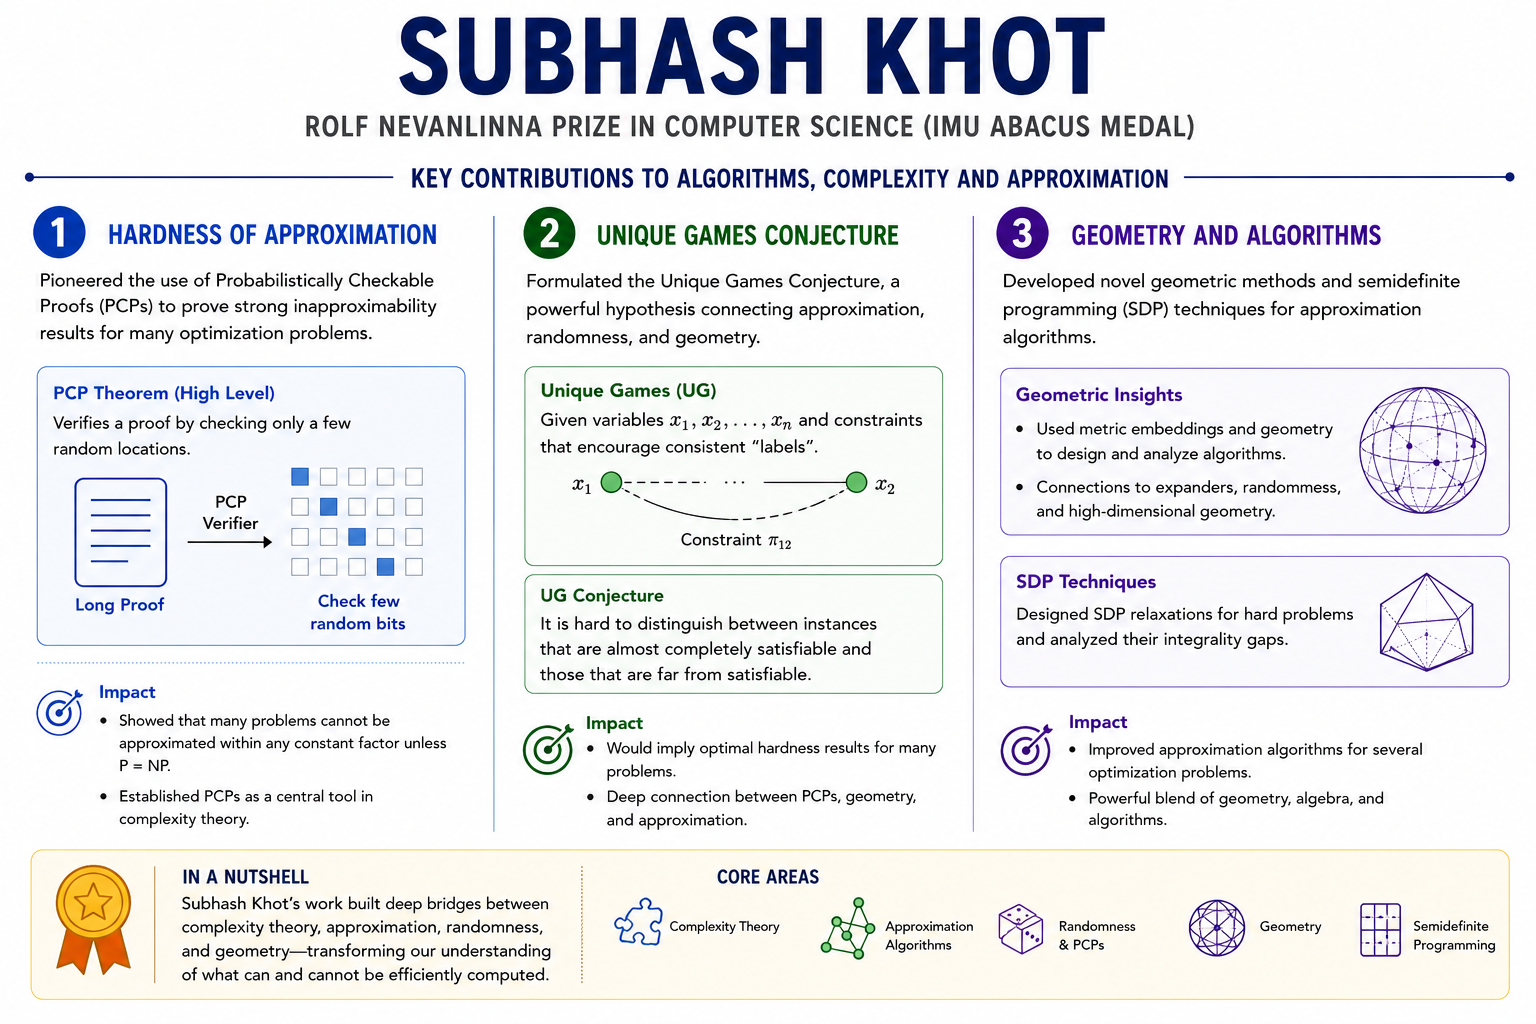
\includegraphics[width=\textwidth]{infographics/abacus9.png}
\end{center}
\targetchapterspacing
\index{Khot, Subhash}

\booknote{The central habit in this chapter is to judge a relaxation by its geometry: the angle between two vectors, not the list of labels, decides which approximation ratio is possible.}

\section{An Opening Story: A Party of Friends With Conflicting Labels}
Four friends---Ana, Bo, Cece, Di---wear tags labeled 0 or 1. Each friendship carries a rule: some pairs must match, others differ. Ana--Bo match, Bo--Cece differ, Cece--Di match, Di--Ana differ. Solution: Ana 0, Bo 0, Cece 1, Di 1.

Change one rule: Di--Ana must match. Walking around the circle forces Di's number to equal Ana's flipped, and to equal Ana's---impossible; the best is three of four rules, 75\%. A thousand friends and ten thousand rules behave the same at scale: each rule satisfiable alone, conflicts colliding around loops. Can a computer tell a party where nearly all rules hold from one where only a tiny fraction do? That question earned Subhash Khot the 2014 Rolf Nevanlinna Prize.

\section{The Problem}
NP-hard problems have no efficient exact algorithm (unless $\mathrm{P}=\mathrm{NP}$), so we accept approximations within a fixed ratio of optimal. Two questions: \emph{what ratio can an algorithm guarantee}, and \emph{what ratio can be proved impossible}? A factor of two may be easy while $1.01$ impossible---not for lack of cleverness but of proof: ruling out ratio $r$ needs instances where the optimum is high, every cheap method is trapped far below it, and a too-good algorithm would solve an NP-hard problem.

Such proofs used to be bespoke; the field wanted one ``mother'' constraint system whose hardness transfers everywhere, and an explanation of why thresholds land exactly where algorithms sit.

\section{The World Before}
\noindent\textbf{Exact optimization is NP-hard.} Since Cook's and Levin's theorems, no efficient exact algorithm exists for essentially every interesting optimization problem; the field retreated to approximation and to proving matching impossibility.

\noindent\textbf{Ratios, problem by problem.} By the early 1990s each problem had its own folklore: scattered, ad hoc proofs producing constants like 2, 1.5, and 0.5, with no unifying explanation.

\noindent\textbf{The PCP theorem.} In the mid-1990s it let every NP proof be checked by a verifier using logarithmically many random bits and querying only a constant number of proof bits; encoded as constraint systems, it became the first general hardness engine. H\aa stad showed MAX-3SAT cannot be beaten past $7/8$, matching the trivial random assignment, but each problem needed a new construction and the tools stalled on two-variable problems like MAX-CUT \cite{hastad-optimal}.

\noindent\textbf{An algorithm at 0.878.} Goemans and Williamson (1995) approximated MAX-CUT within $0.878$ via vectors and a random hyperplane. Unconditional PCP hardness reached only $16/17\approx0.941$; the matching $0.878+\eps$ was beyond the technology, and $0.878$ had no advance explanation \cite{goemans-williamson,hastad-optimal}.

\noindent\textbf{What was missing.} A single conjectured base problem whose hardness transfers everywhere, and a language in which the transfer is automatic. Khot supplied both; the base problem is Unique Games.

\section{The New Idea}
\subsection{A puzzle whose edges are permutations}
A \emph{unique game} is the party puzzle at scale. Vertices carry labels from $[k]$; each edge $(u,v)$ carries a bijection $\pi_e$ demanding $\pi_e(\text{label of }u)=\text{label of }v$. With two labels a permutation is just ``same'' or ``flip.'' Each constraint is one-to-one: fix one endpoint's label and the other's is forced. Every edge is locally trivial, so all difficulty is global, hidden in how permutations compose around cycles.

\subsection{The promise that makes it hard}
The Unique Games Conjecture (2002) concerns a \emph{promise problem}: the instance is either nearly perfect---at least $1-\delta$ of edges satisfiable---or almost empty---at most $\eps$---for tiny $\delta,\eps>0$. The conjecture: for every $\eps,\delta>0$ some label set size $k$ makes \emph{distinguishing the two cases NP-hard}. Fully satisfiable instances are easy on each connected component (guess one label per component and propagate); the difficulty is detecting global consistency when local demands never conflict \cite{khot-unique}.

\subsection{Why the seed is so powerful}
If problem $P$ reduces \emph{from} Unique Games, the promise survives: yes-instances become $P$-instances of value at least $c$, no-instances of value at most $s$. Any algorithm with approximation factor strictly better than $c/s$ would separate the cases. Because reductions are engineered outward from the game, $c/s$ can be tuned to targets like $0.878+\eps$: one hard promise, many exact thresholds.

\subsection{The geometry that fixes the threshold}
The companion tool is the \emph{semidefinite relaxation}. In the Boolean/MAX-CUT case, labels become unit vectors and constraints become angle statements. Rounding returns vectors to labels via a random hyperplane; an edge's survival probability depends only on the angle $\theta$ via $\theta/\pi$. For general Unique Games, the SDP instead uses vector variables for vertex-label pairs together with orthogonality and consistency constraints. The \emph{invariance principle}---high-dimensional discrete systems with no dominant variable behave like Gaussians---carries the game's discrete hardness into Gaussian geometry, where landmark thresholds can be computed exactly and matched to the best-known algorithms.

The conceptual shift: \emph{a single carefully designed constraint system can be the seed of hardness for many optimization problems; the geometry of the relaxation determines the threshold.}

\section{How It Works: Worked Examples}
\subsection{Two four-person parties, label by label}
Friends $A,B,C,D$; labels $\{0,1\}$; rules as equations $x_j=x_i\oplus b_{ij}$:
\begin{center}
\begin{tabular}{llc}
\toprule
Edge & Rule & Equation \\
\midrule
$(A,B)$ & same & $x_B=x_A$ \\
$(B,C)$ & flip & $x_C=x_B\oplus1$ \\
$(C,D)$ & same & $x_D=x_C$ \\
$(D,A)$ & flip & $x_A=x_D\oplus1$ \\
\bottomrule
\end{tabular}
\end{center}
Set $x_A=0$ and walk around: $x_B=0$, $x_C=1$, $x_D=1$, and the last rule needs $x_A=x_D\oplus1=0$---consistent. Two flips around the loop, and $0\oplus1\oplus1=0$; $(0,0,1,1)$ satisfies all four rules.

Instance 2: change the last rule to ``same,'' $x_A=x_D$. The walk gives $x_D=x_A\oplus1$, and the last rule demands $x_A=x_D=x_A\oplus1$---contradiction for either value of $x_A$. Each of the four assignments fails exactly one edge, so the best is $3/4=75\%$.

One flip instead of two. With two labels a cycle is fully satisfiable exactly when its flip count is even; with $k$ labels: \emph{the permutations around every cycle must compose to the identity}. Local constraints are individually satisfiable; only the product of permutations around closed walks decides global feasibility, and a label-recovery problem is hard precisely when this consistency is hard to detect.

\subsection{MAX-CUT: vectors, then a random wall between them}
MAX-CUT partitions a graph's vertices into two sides to maximize crossing edges---the two-label puzzle again, each edge demanding $x_u\ne x_v$.

The SDP relaxation assigns each vertex $i$ a unit vector $v_i$ and maximizes
\[
\sum_{(i,j)} \frac{1-v_i\cdot v_j}{2}.
\]
Rounding: pick a uniformly random direction $r$; put $i$ on the side $\operatorname{sign}(r\cdot v_i)$. Edge $(i,j)$ is cut when the signs disagree, with probability depending only on $\theta=\arccos(v_i\cdot v_j)$:
\[
\Pr[\text{cut}]=\frac{\theta}{\pi}.
\]
Three checks: $v_i\cdot v_j=0$ ($\theta=\pi/2$) gives $1/2$; $v_i=v_j$ ($\theta=0$) gives $0$; $v_i=-v_j$ ($\theta=\pi$) gives $1$.

At the worst angle, $\theta^*\approx0.74\pi$ (about $133^\circ$, $\cos\theta^*\approx-0.69$): the SDP contribution is $(1-(-0.69))/2\approx0.845$, but rounding cuts the edge with probability only $0.74$. The ratio $0.74/0.845\approx0.878$ is the minimum of $(\theta/\pi)\big/\big((1-\cos\theta)/2\big)$ over all angles---exactly the Goemans--Williamson factor. Their theorem: for \emph{every} graph, rounding any SDP solution cuts, in expectation, at least $0.878$ times the SDP value, hence $0.878$ times the optimum. Under Unique Games, beating $0.878+\eps$ is impossible (Khot, Kindler, Mossel, O'Donnell) \cite{goemans-williamson,khot-hardness}.

\section{The Mathematics in Brief}
\emph{The instance.} A Unique Game is a graph $(V,E)$ with label set $[k]$; each edge $e=(u,v)$ carries a bijection $\pi_e:[k]\to[k]$; an assignment $a$ satisfies $e$ when $\pi_e(a_u)=a_v$. Cycles are consistent exactly when their permutations compose to the identity.

\emph{The promise.} Distinguish $(1-\delta)$-satisfiable (some assignment satisfies $\ge1-\delta$ of the edges) from $\eps$-satisfiable (every assignment satisfies $\le\eps$). UGC: for every $\eps,\delta>0$ this is NP-hard for some label set size $k$.

\emph{The gap reduction.} If a reduction from Unique Games to $P$ preserves completeness $c$ and soundness $s$, no algorithm with approximation factor strictly better than $c/s$ can exist under UGC, or it would separate the cases.

\emph{MAX-CUT.} Relax to $\max\sum(1-v_i\cdot v_j)/2$ over unit vectors; round by a random hyperplane with $\Pr[\text{cut}]=\theta/\pi$. The inequality $\theta/\pi\ge\alpha(1-\cos\theta)/2$ with $\alpha\approx0.878567$ yields the approximation factor, and UGC-hardness rules out $\alpha+\eps$: the bounds meet.

\emph{The invariance principle.} A low-degree multilinear polynomial of many weakly correlated discrete variables with no dominant variable is distributed nearly like the same polynomial on Gaussians with matching correlations---many small independent contributions converge to a Gaussian. It moves hardness from discrete games into Gaussian space, where isoperimetric theorems can compute sharp thresholds.

\section{Limits and Modern Views}
\emph{A conjecture, not a theorem.} UGC remains open, so results conditional on it must be labeled as such; some stronger formulations were disproved. The neighbouring \emph{2-to-2 Games Conjecture} (constraints two-to-two instead of one-to-one) was completed in 2018 in an imperfect-completeness form through work by Khot, Minzer, and Safra, building on the reduction and framework of Dinur, Khot, Kindler, Minzer, and Safra. It yields unconditional hardness results for vertex cover approaching $\sqrt2$ (beyond the long-standing $1.36$ bound) and for independent set, and strengthens belief in UGC \cite{dkkms-2to2,kms-2to2}. Specialized families are understood; the general promise is not.

\emph{Unconditional gaps are weaker.} An integrality gap shows one relaxation cannot certify a better ratio; it says nothing about stronger algorithms, while UGC hardness would settle the question.

\emph{Structure beats worst cases.} Hardness is worst-case; sparse graphs, clustered data, and inputs with known distributions carry structure algorithms exploit. The right response to a barrier is diagnosis: ask what the fractional solution knows, what the integral solution requires, and which correlation the rounding step forgot.

\emph{Where the field went.} Sum-of-squares hierarchies seek stronger relaxations; spectral and local algorithms exploit expansion; and, assuming UGC, Raghavendra showed that the best polynomial-time ratio for every constraint satisfaction problem is characterized by the geometry of a suitable SDP relaxation \cite{raghavendra-csp}.

\section{Exercises and Self-Study Guide}
\begin{enumerate}[label=\textbf{E\arabic*.}]
\item Verify both party instances by writing out all four assignments; then build a five-vertex cycle with exactly two flips and show it is fully satisfiable.
\hint{A two-label cycle is satisfiable exactly when its flip count is even; fix one label and propagate.}
\item Explain how the promise---``$(1-\delta)$- or $\eps$-satisfiable''---differs from ``is this instance fully satisfiable?'', and why the latter is easy.
\hint{A promise problem answers only on the two guaranteed input kinds; a fully satisfiable unique game is solved by propagating one guessed label.}
\item For vectors with $v_i\cdot v_j=1/2$ and $v_i\cdot v_j=-1/2$, compute the angle $\theta$, the SDP contribution $(1-v_i\cdot v_j)/2$, and the cut probability $\theta/\pi$. Which angle loses more?
\hint{$\arccos(1/2)=\pi/3$: cut probability $1/3$, contribution $1/4$, ratio $4/3$; only near $\theta^*\approx0.74\pi$ does the ratio fall to $0.878$.}
\item A gap reduction has completeness $c=0.9$ and soundness $s=0.3$. If an algorithm returns at least $\mathrm{OPT}/r$, which $r$ separate yes from no by output size?
\hint{Separation needs $0.9/r>0.3$, so $r<3$; in general the factor ruled out is $c/s$.}
\item Identify a global property of the party cycle that a local pairwise relaxation cannot express.
\hint{Each flip is locally satisfiable by half of all label pairs; only the product of permutations around a loop records feasibility.}
\item Build a tiny integer program whose relaxation beats the integral optimum: cover the triangle, $x_A+x_B\ge1$, $x_B+x_C\ge1$, $x_A+x_C\ge1$, minimize the sum, $x_i\in\{0,1\}$.
\hint{$(1/2,1/2,1/2)$ costs $1.5$; every integral cover costs $2$.}
\item Give a rounding rule that preserves every marginal but violates a pairwise ``must be equal'' constraint with positive probability.
\hint{Independent rounding to 0 with probability $p$: marginals match, but two forced-equal variables agree only with probability $p^2+(1-p)^2$.}
\end{enumerate}

\booknote{A final exercise in judgment: whenever a relaxation seems to declare a problem easy, ask what the fractional solution knows, what the integral solution requires, and which correlation the rounding step forgot.}
\clearpage

\chapter{2018:Constantinos Daskalakis}
\label{chap:daskalakis}
\begin{center}
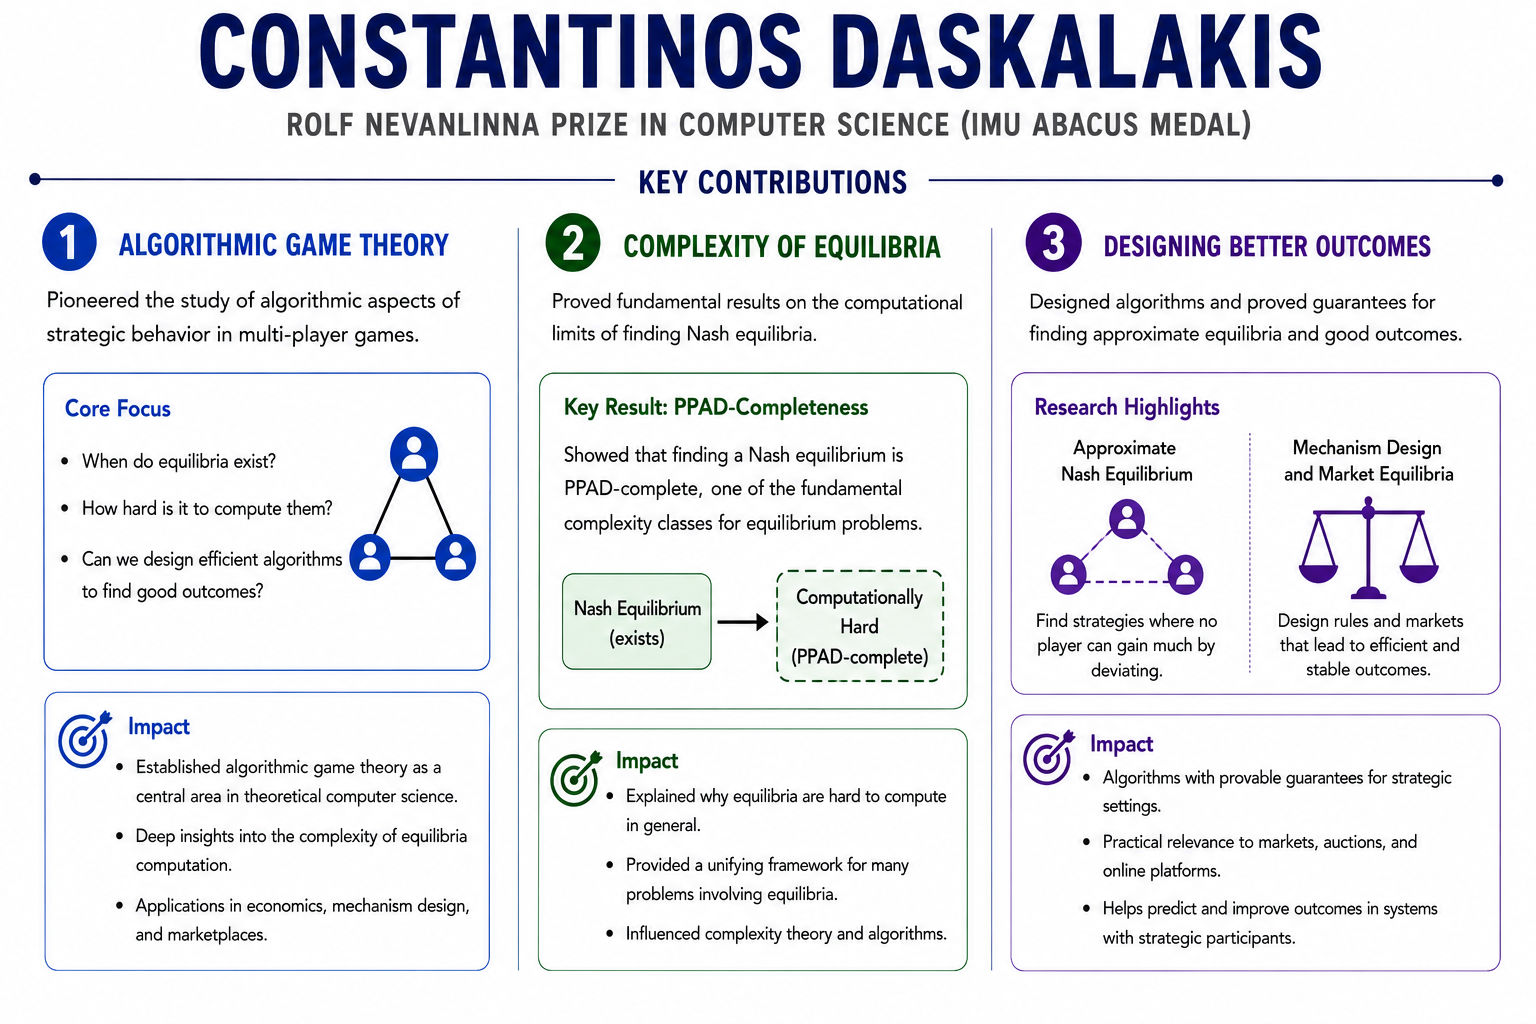
\includegraphics[width=\textwidth]{infographics/abacus10.png}
\end{center}
\targetchapterspacing
\index{Daskalakis, Constantinos}
\booknote{The central habit in this chapter is to keep existence and computation apart: a theorem that a solution exists is not an algorithm for finding it.}

\section{An Opening Story: A Price War Between Two Sellers}

Two coffee sellers, Priya and Malik, face each other across the same street. Each morning each posts a price for a latte, and each profit depends on the other's price: undercut by a dollar and the commuters drift to your window. So each seller's \emph{best} price is a moving target---whatever beats the other's price of yesterday. Starting from \$5 and \$5, Priya drops to \$4.50, Malik answers at \$5.25, Priya drops to \$4.25. They may settle on a stable pair, bounce forever, or wander.

A theorem guarantees a stable pair of prices exists: at some pair, neither seller, facing the other's price, would change anything. But the theorem does not say how to find it, nor what a month of daily adjustments will do. \emph{A stable pair exists} and \emph{here is how to find it} are different claims. This chapter is about the difference.

\section{The Problem}

In a game, each player's best choice depends on everyone else's. A \emph{Nash equilibrium} is a collection of choices---possibly random, since a player may prefer to mix---such that nobody can improve by changing alone. Nash proved in 1950 that every finite game has an equilibrium. That settled existence. The problem here is \emph{computation}: given the rules of a game, find an equilibrium. Existence and calculation are different questions, and a well-defined solution need not be algorithmically accessible.

\section{The World Before}

\noindent\textbf{Nash's proof was non-constructive.} Best responses form a set-valued correspondence rather than a continuous map, so the standard existence proof uses Kakutani's fixed-point theorem (or an equivalent continuous reformulation). The theorem guarantees an equilibrium in the compact convex region of mixed-strategy profiles but gives no recipe for locating it.

\noindent\textbf{Economists treated equilibria as predictions.} The equilibrium of a market---prices where supply meets demand---was a forecast, on the implicit assumption that players or markets would reach it. For decades nobody asked whether anyone or any algorithm could actually find one.

\noindent\textbf{Pivoting algorithms worked in practice.} The Lemke--Howson algorithm and its relatives find equilibria of two-player games by walking around the polytope of profiles. They solve small games quickly, but carry no general guarantee: some games force exponentially long walks.

\noindent\textbf{Continuous space, discrete search.} Brouwer's theorem lives in a continuous region; a computer searches a finite structure, and a grid does not help: a fixed point can sit between grid points, and the grid has exponentially many cells.

What was missing was a language for the difficulty of problems whose solutions are \emph{guaranteed} to exist. Classes like NP capture ``hard to decide''; for search problems with a promised answer, no comparable class existed, nor the reduction machinery to prove one such problem as hard as any other. Those tools were what Daskalakis and his collaborators supplied.

\section{The New Idea}
\subsection{The path picture: PPAD}

Consider a directed graph where every node has at most one arrow in and at most one arrow out. Such finite graphs split into paths and cycles. A node with no arrow entering is a \emph{source}; one with no arrow leaving is a \emph{sink}. Handed a source, following arrows must stop at a sink: the graph is finite, and a revisit would give some node a second incoming arrow---forbidden. The ends of paths come in pairs, and you were given one end.

Now make the graph \emph{implicit}: $2^k$ nodes, not listed, with a small circuit reporting each node's predecessor and successor. This is the setup of \textbf{PPAD} (Polynomial Parity Argument on Directed graphs): total search problems whose solution is guaranteed by exactly this parity/path argument. Given one endpoint of a path, find another---a node whose indegree differs from its outdegree. Following the path always works but may take $2^k$ steps.

\subsection{Nash equilibrium is PPAD-complete}

Daskalakis, Goldberg, and Papadimitriou showed that a game can encode the successor circuit of a PPAD problem: they built games with three or more players whose Nash equilibria encode the ``other end of the path'' of any PPAD instance, so finding an equilibrium is at least as hard as finding that endpoint. Chen and Deng extended this to two-player games; Chen, Deng, and Teng, even to \emph{approximate} equilibria when the allowed error is small. This was the first natural problem known to combine guaranteed existence with provable hardness of search. The difficulty is not a missing algorithm; it is a structural property of the problem class.

\subsection{The same framework, elsewhere}

The reduction template spread to market equilibria, auction bidding, and mechanism design: a solution exists by a fixed-point or parity argument, but computing it is hard in general. Not a blanket claim of hopelessness---special cases have fast algorithms: two-player zero-sum games solve by linear programming; potential games settle under any improving best responses; few players, limited interaction, or special payoffs admit dedicated algorithms. \emph{Easy structure versus hard general case is the whole point.}
\emph{The conceptual shift: a theorem that a solution exists is not an algorithm for finding it, and a problem can be guaranteed-solvable in principle yet provably intractable to search.}

\section{How It Works: Worked Examples}
\subsection{Matching pennies: finding the mixed equilibrium}

Row and Col each choose Heads ($H$) or Tails ($T$). Row receives $+1$ when the choices match and $-1$ when they differ; Col receives the opposite. This zero-sum game has no pure equilibrium: whichever pair you pick, one player wants to switch.

Let Row play $H$ with probability $p$. Against Col's $H$, Row's expected payoff is $p(+1)+(1-p)(-1)=2p-1$; against Col's $T$, it is $p(-1)+(1-p)(+1)=1-2p$. For Col to be willing to mix, Col must be indifferent between $H$ and $T$, so
\[
2p-1=1-2p \quad\Longrightarrow\quad 4p=2 \quad\Longrightarrow\quad p=\tfrac12,
\]
and by symmetry Col also plays $H$ with probability $\tfrac12$.

The equilibrium: both randomize 50/50, each with expected payoff $2p-1=0$. Check it: if Row switches to pure $H$ while Col randomizes, Row's expected payoff is $\tfrac12(+1)+\tfrac12(-1)=0$---no gain. Nobody can improve by deviating, which is the definition of equilibrium. Note the \emph{indifference principle}: at equilibrium, every action played with positive probability must give equal expected payoff, or the player would shift probability to the better one.

\subsection{The PPAD path: existence you can feel but not always walk}

Nodes $0,1,2,3,4$; edges $0\to1$, $1\to2$, $3\to4$. The graph is implicit: a successor circuit answers node by node,
\[
\operatorname{succ}(0)=1,\ \operatorname{succ}(1)=2,\ \operatorname{succ}(2)=\varnothing,\ \operatorname{succ}(3)=4,\ \operatorname{succ}(4)=\varnothing,
\]
with consistent predecessors $\operatorname{pred}(1)=0$, $\operatorname{pred}(2)=1$, $\operatorname{pred}(4)=3$. Sources (no incoming edge): $0$ and $3$; sinks (no outgoing edge): $2$ and $4$. Given source $0$, follow: $\operatorname{succ}(0)=1$, $\operatorname{succ}(1)=2$, $\operatorname{succ}(2)=\varnothing$. The walk stops at $2$: the other end. Two sources, two sinks---ends of paths come in pairs, so knowing one end guarantees another exists.

Why hard? Here the whole graph is drawn, so the answer is obvious. In a real instance the graph has $2^k$ nodes presented only through the circuits: you evaluate them one node at a time, never seeing the whole graph, and the path from your source can have length $2^k$. Walking it takes $2^k$ steps, though the guarantee that the other end exists is airtight. When the successor circuit encodes another hard problem, locating the other end is provably as hard as solving it.

\section{The Mathematics in Brief}

A \emph{finite game} has $n$ players with finite action sets $A_i$. A \emph{mixed strategy} for player $i$ is a distribution $x_i$ over $A_i$; a \emph{profile} $x=(x_1,\dots,x_n)$ collects one per player, giving expected payoff $u_i(x)$. Strategy $x_i$ is a \emph{best response} when $u_i(x_i,x_{-i})\ge u_i(y_i,x_{-i})$ for every $y_i$. A \emph{Nash equilibrium} is a profile where everyone plays a best response---a fixed point of the best-response correspondence. \emph{Why existence is true:} profiles form a compact convex region, each best-response set is nonempty and convex, and the correspondence is upper hemicontinuous; Kakutani's theorem supplies a fixed point.

The \emph{indifference principle} is the workhorse: at equilibrium, actions used with positive probability give equal expected payoff; worse actions get probability zero.

\textbf{PPAD} is the class of total search problems whose guaranteed solution follows from a path/parity argument on an implicitly defined graph: indegree and outdegree each $\le1$; given a source, find a node whose indegree differs from its outdegree. \emph{Why the guarantee holds:} following the unique path from a source cannot loop, so it must reach a sink.

\textbf{The completeness theorem.} Computing a Nash equilibrium of a game with three or more players is PPAD-complete (Daskalakis--Goldberg--Papadimitriou), and remains so for two-player games and even for \emph{approximate} equilibria (Chen--Deng; Chen--Deng--Teng). An $\varepsilon$-equilibrium is a profile where $u_i(x_i,x_{-i})+\varepsilon\ge u_i(y_i,x_{-i})$ for all $y_i$: nobody gains more than $\varepsilon$ by deviating. \emph{Why:} games can encode successor circuits, so an equilibrium encodes the endpoint of a hidden path. \emph{Consequence:} worst-case hardness coexists with fast algorithms on structured instances, and with learning dynamics that may converge to outcomes that are not equilibria.

\section{Limits and Modern Views}

PPAD-completeness is a \emph{worst-case} statement, asymptotic in game size. It does not say real markets are unsolvable: practical instances usually carry structure---few players, symmetric payoffs, sparse interaction---that dedicated algorithms exploit.

Approximation does not dissolve the difficulty: an $\varepsilon$-equilibrium is hard when the required precision is part of the input, and the smaller the error, the more of the hard problem the game encodes. Discretization is no escape: replacing a continuous strategy space by a finite grid changes the game, and the discrete equilibria need not lie near the continuous ones. Learning dynamics may cycle or settle into stable non-equilibrium outcomes---for prediction, those may matter more than the equilibrium itself, shifting the question from \emph{what is the equilibrium?} to \emph{what outcomes can plausible processes generate?}

The field that grew from these results is \emph{algorithmic economics}: auctions and mechanisms where truthfulness, feasibility, and computation fit together. Optimal transport supplies a geometric language for some mechanism-design problems, dual potentials playing the role of prices. The deep lesson: social concepts have computational structure---equilibrium, incentive compatibility, and optimal allocation are algorithmic tasks whose representations determine what can be found, approximated, or predicted \cite{daskalakis-nash,daskalakis-markets}.

\section{Exercises and Self-Study Guide}
\begin{enumerate}[label=\textbf{E\arabic*.}]
\item Biased matching pennies: Row gains $+3$ when both play $H$, $+1$ when both play $T$, $-1$ on a mismatch; Col's payoffs are the negatives. If Row plays $H$ with probability $p$ and Col with probability $q$, find the equilibrium $(p,q)$ and Row's expected payoff.
\hint{Col's mix $q$ must make Row indifferent: equate $q(+3)+(1-q)(-1)$ with $q(-1)+(1-q)(+1)$; then use $p$ to make Col indifferent.}
\item In ordinary matching pennies, show (both play $H$) is an $\varepsilon$-equilibrium for $\varepsilon=2$ but not an equilibrium, and that no pure profile is an equilibrium.
\hint{At $(H,H)$ Row gets $+1$, Col $-1$; compute the best each could do by switching alone and take the larger gain.}
\item Explain why Nash's fixed-point existence proof gives no search algorithm.
\hint{Brouwer guarantees a point but no path to it; a grid search either misses it or faces exponentially many cells.}
\item Trace best-response dynamics in matching pennies from $(H,H)$ and show the play cycles forever.
\hint{Row copies Col and Col plays the opposite: $(H,H)\to(H,T)\to(T,T)\to(T,H)\to(H,H)$.}
\item A seller's price is continuous in $[4,7]$ with unique equilibrium $\$5.37$. Explain how forcing prices onto the grid $\{4,5,6,7\}$ can change the equilibrium.
\hint{The grid game allows different deviations and output points; the continuous equilibrium may lie strictly between grid lines.}
\item No-regret learners in matching pennies never settle, yet their empirical frequencies converge to the equilibrium mix. Why is stable frequency compatible with unstable play?
\hint{Regret compares accumulated average payoff with the best fixed action; in a zero-sum game the frequencies encode the equilibrium while realized actions alternate.}
\item Pick one assumption a market or mechanism-design model relies on---quasi-linear utilities, a known type distribution, or fully rational agents---and explain what happens to the complexity analysis if it is removed.
\hint{Ask which part of the argument used it: a truthfulness proof needs quasi-linear utility, a hardness reduction needs structure encoding arbitrary instances---removing it reopens the complexity question.}
\end{enumerate}

\booknote{A final exercise in judgment: whenever you are told that a solution exists, ask separately how a machine would find it, how the answer would be verified with a certificate, and whether the guarantee survives approximation. If you cannot name the certificate, the existence proof is not yet an algorithm.}
\clearpage

\chapter{2022:Mark Braverman}
\label{chap:braverman}
\begin{center}
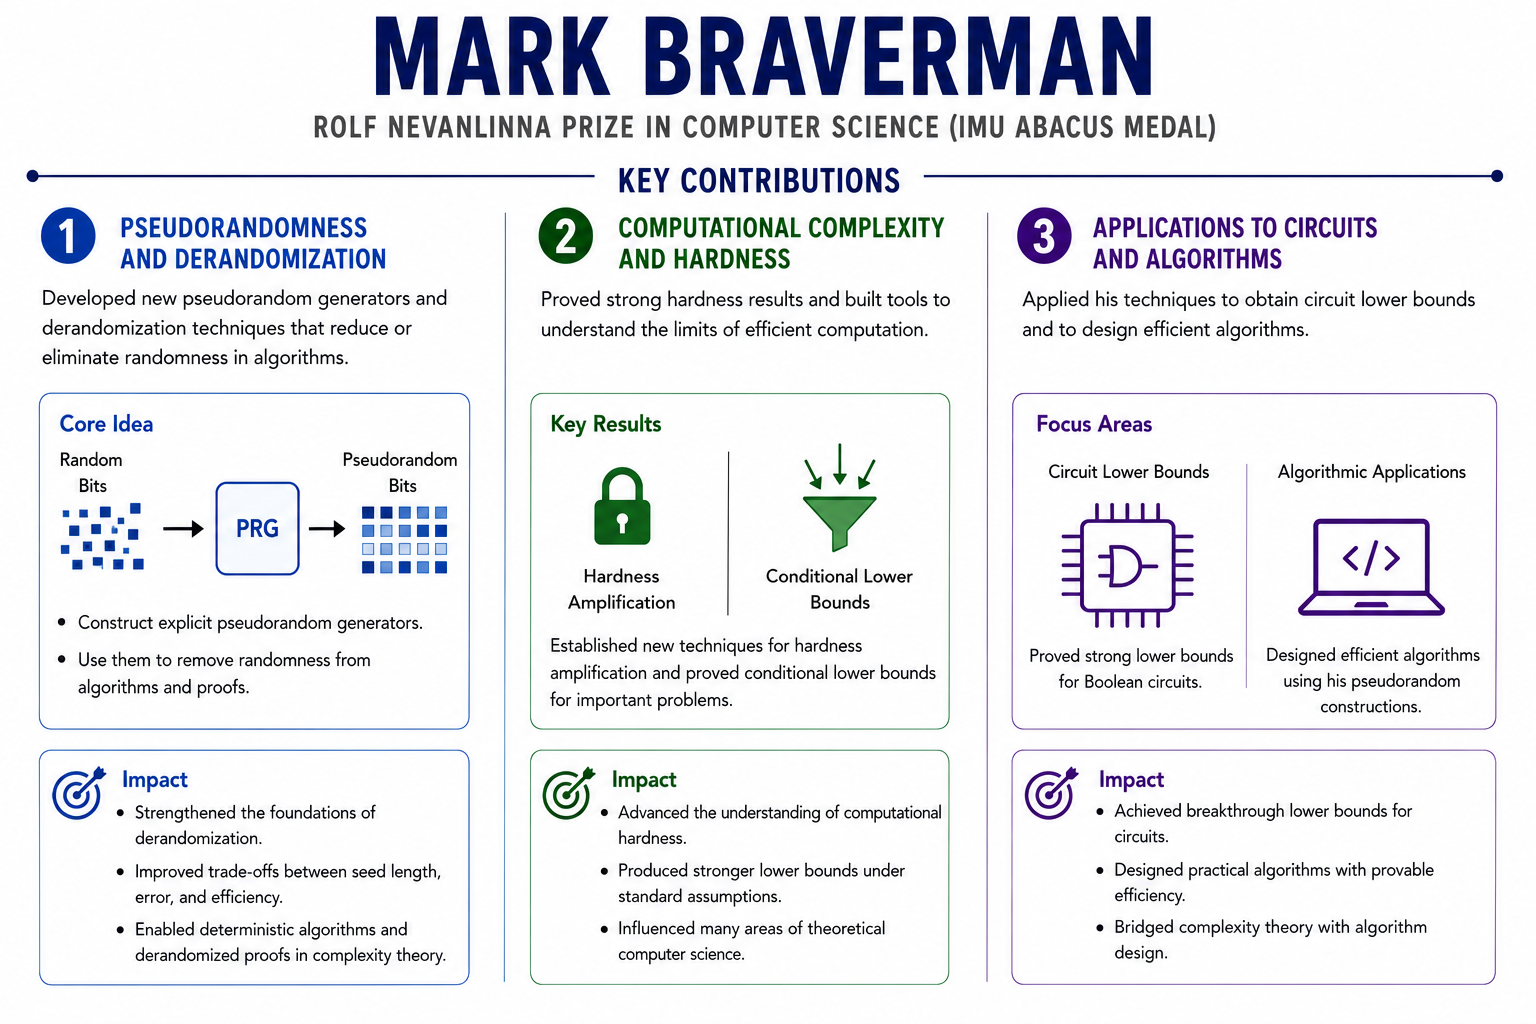
\includegraphics[width=\textwidth]{infographics/abacus11.png}
\end{center}
\normalchapterspacing
\index{Braverman, Mark}
\booknote{The central habit in this chapter is to ask not only what a protocol communicates, but what uncertainty it must destroy before the communication can succeed.}

\section{An Opening Story: The Party That Never Happened}
Two friends, Alice and Bob, sit in separate rooms planning a party. Each has privately decided whether they can come: a card reads ``0'' (no) or ``1'' (yes), and the party is worth planning only if \emph{both} cards read 1. They must agree on the answer, but every text message costs one coin, and they want to spend as few coins as possible. The obvious plan costs two coins: Alice texts her card, Bob texts his. But watch what actually happens. If Alice's card reads 0, the party is already off and Bob's answer changes nothing---the second coin buys nothing at all. The smarter plan is for Alice to text first and for Bob to text only if her card reads 1. Then two coins are needed only when her card reads 1, which happens half the time; on the other half, one coin settles everything.

Now suppose the pack is rigged so that 0-cards are ninety-nine times more common than 1-cards. The second message almost never matters, yet a worst-case budget of two coins still stands. A planner who pays typical costs spends a bit over one coin; an accountant who charges for \emph{information removed} rather than symbols sent demands only about a tenth of a coin. Three currencies, three prices for the same conversation. Deciding which price is honest, and learning to compute it, is the subject of this chapter---the work for which Mark Braverman received the 2022 Abacus Medal.

\section{The Problem}
Alice knows a private input $x$; Bob knows a private input $y$. By exchanging messages according to an agreed protocol, they must compute a function $f(x,y)$---for the party, ``do both cards read 1?''---correctly on every pair of inputs. The classical question is easy to state: how many bits must they exchange in the worst case? The deeper question is harder: what is each bit doing?

A transcript is not just a string; it is a sequence of decisions made under partial knowledge. Alice's message can reveal her card, rule out a whole class of worlds, coordinate a shared random experiment, or merely confirm an event Bob already believed. Counting symbols treats all four uses as equal, like pricing a house by counting its bricks. Two conversations of the same length can have radically different value: one message splits two equally likely worlds, another confirms a world already $99\%$ certain. The field's hardest open problems were about composition---must many independent copies cost many times one copy?---and about leakage: how much does a transcript reveal? Worst-case length could not answer either question.

So ``how many bits?'' and ``how much does the conversation buy?'' are different questions, and the party protocol is a microscope for the difference. The first message (Alice's card) always matters; the second (Bob's, sent half the time) matters only conditionally. A correct measure must charge them differently and let a long but nearly empty conversation cost almost nothing.

\section{The World Before}
Yao's 1979 model fixed the vocabulary: two players, private inputs, agreed rules, and a cost measured as the worst-case number of bits exchanged. The communication complexity $D(f)$ is the smallest worst-case length of any correct protocol, and the field built its power from lower-bound tools proving that specific functions genuinely need many bits.

Two tools dominated. A \emph{fooling set} is a collection of input pairs that all demand separate transcripts: if $(x,y)$ and $(x',y')$ both map to output 1 but the crossed pairs $(x,y')$ and $(x',y)$ map to 0, then no two of them can share a conversation, so the protocol needs at least as many distinct transcripts as the set has elements. The \emph{rank method} is more algebraic: write $f$ as a matrix with rows $x$, columns $y$, entries $f(x,y)$. Every deterministic protocol carves the matrix into monochromatic rectangles, one per transcript, and each rectangle is rank-1. A binary protocol of depth $t$ has at most $2^t$ transcripts, so $2^t$ is at least the matrix's rank. For equality of two $n$-bit strings the matrix is the $2^n\times 2^n$ identity, of rank $2^n$; hence at least $n$ bits are needed, and $n$ suffice. These tools are sharp, elegant, and measure only length.

The tools shared a blind spot: they could not explain why a long protocol might be nearly free. The party protocol has worst-case length 2 bits, yet on a typical conversation its second message is empty and even on the long branch it says one obvious thing; there was no vocabulary for ``this message was nearly predictable.'' Worst-case counting also could not amortize: for deterministic protocols $k$ copies trivially cost $k$ times one copy, but the honest average cost per copy over a stream of independent copies, where randomized protocols may share randomness, had no sharp answer---and neither did the question of how much information a transcript leaks about the inputs. A field built to answer ``how much must they say'' had no language for ``how much is revealed.''

The missing tool was a measure of communication that (i) decomposes round by round, (ii) adds over independent copies, and (iii) can be compared with transcript length. Information theory already had (i) and (ii) in entropy and the chain rule; the creative step was to point that machinery at interactive protocols and make the transcript itself the random variable being measured. The right unit of thought was not the symbol but the uncertainty destroyed.

\section{The New Idea}
The change of unit, in one sentence: charge a protocol for the information its transcript reveals about the inputs, not for the symbols it sends. A message the receiver could already predict is free; a message that splits the remaining uncertainty is expensive. This is the \emph{internal information cost} of the protocol,
\[
\operatorname{IC}_\mu(\Pi)=I(X;\Pi\mid Y)+I(Y;\Pi\mid X),
\]
where $\Pi$ is the random transcript and the conditioning records what each party already knows: Alice holds $X$, Bob holds $Y$, and information already sitting on its own side of the border is not charged for crossing it. (With public randomness $R$ shared by both, condition on $R$ too, since the shared coin is free.) The conditioning is not cosmetic: it is what makes the party protocol cost $3/2$ bits instead of $2$, as the worked example will show.

Three consequences follow from this unit.

\subsection{Compression: little information means few bits}
If a protocol reveals almost nothing, its transcript should be reproducible with almost no communication. From Bob's point of view, Alice's message is a sample from a distribution she can compute; with shared randomness, both players can search the random tape for that sample together, paying only for the part Bob could not have predicted. The compression principle states that a transcript of internal information cost $c$ can be simulated with communication proportional to $c$, up to overhead growing with rounds and error. Its sharpest form, Braverman--Rao's \emph{information equals amortized communication}, is an equality: the honest per-copy cost of many independent copies of a function is exactly the internal information cost of one copy.

\subsection{Direct sums: copies add up}
If one copy needs information $c$, then $k$ independent copies need $kc$. This direct-sum statement looks obvious and is the entire point: information, unlike worst-case length, satisfies the additivity amortized reasoning demands. Independent coordinates contribute independently to the transcript's information---the machinery is the chain rule. The subtlety is that conditioning on a whole transcript can couple coordinates that started independent; the fix is a random-coordinate embedding that converts the $k$-copy protocol into a one-copy protocol of the same per-copy cost.

\subsection{Noise: checkpoints and entangled correction}
Real channels flip bits, and one corrupted message changes the meaning of every later message: the parties may silently disagree about which history they share. Error correction cannot be bolted on beneath the computation, since the players may not even agree on what to correct. Robust interactive protocols must create checkpoints---frequent cheap confirmations that both parties stand on the same transcript---so computation and correction become entangled. In standard interactive-coding models with a fixed noise rate below the permitted threshold, Braverman and collaborators showed that a protocol of length $n$ can be simulated with only a constant-factor communication overhead and arbitrarily small error. The exact guarantee depends on the channel, noise rate, and feedback assumptions; the information viewpoint turned a believed polylogarithmic overhead into a constant.

\section{How It Works: Worked Examples}

\subsection{A warm-up: how much does a noisy coin flip tell us?}
Let $X$ be a fair bit, so $H(X)=1$. Suppose a friend tells us the value of $Z$, obtained by flipping $X$ with probability $p$: if $X=0$ then $Z=1$ with probability $p$; if $X=1$ then $Z=0$ with probability $p$. How much do we learn about $X$ by hearing $Z$?

Write $H(p)=-p\log_2 p-(1-p)\log_2(1-p)$ for the binary entropy function. Given $X$, the observation $Z$ is a coin flip with bias $p$, so $H(Z\mid X)=H(p)$. Meanwhile $Z$ is still a fair bit overall, because flipping a fair coin with probability $p$ leaves it fair: $H(Z)=1$. Therefore
\[
I(X;Z)=H(Z)-H(Z\mid X)=1-H(p).
\]
Check the endpoints. If $p=0$ then $H(0)=0$ and $I=1$: $Z$ always equals $X$, so hearing $Z$ reveals $X$ completely. If $p=1/2$ then $H(1/2)=1$ and $I=0$: $Z$ is a fresh fair coin flip, statistically independent of $X$. Now one interior value. For $p=1/4$,
\[
H(1/4)=-\tfrac14\log_2\tfrac14-\tfrac34\log_2\tfrac34=\tfrac12+\tfrac34(0.415)\approx 0.811,
\]
using $\log_2 4=2$ and $\log_2(3/4)=\log_2 3-2\approx -0.415$. So a $3/4$-reliable observation is worth $I(X;Z)\approx0.189$ bits---less than a fifth of a bit, because most of what it says was already predictable. That is the first concrete lesson of the chapter.

\subsection{The two-bit AND protocol: a conversation worth $3/2$ bits}
Return to the party. $X$ and $Y$ are independent fair bits, and the protocol is the smart one: Alice sends $X$; if $X=1$, Bob sends $Y$; if $X=0$, Bob sends nothing. The three possible transcripts and their probabilities are:
\begin{center}
\begin{tabular}{lcc}
\toprule
Transcript & Input & Probability \\
\midrule
``0'' & $X=0$ & $1/2$ \\
``1,0'' & $X=1$, $Y=0$ & $1/4$ \\
``1,1'' & $X=1$, $Y=1$ & $1/4$ \\
\bottomrule
\end{tabular}
\end{center}
Compute the internal information cost by hand, one term at a time.

\emph{Alice's contribution.} For $I(X;\Pi\mid Y)$, fix $Y=0$. Then $X$ is still a fair bit, so $H(X\mid Y=0)=1$, and the transcript determines $X$: ``0'' means $X=0$, ``1,0'' means $X=1$. Thus $H(X\mid \Pi,Y=0)=0$ and $I(X;\Pi\mid Y=0)=1$. The same with $Y=1$ gives $I(X;\Pi\mid Y=1)=1$, so averaging over $Y$,
\[
I(X;\Pi\mid Y)=\tfrac12\cdot 1+\tfrac12\cdot 1=1.
\]

\emph{Bob's contribution.} For $I(Y;\Pi\mid X)$, split by $X$. If $X=0$, the transcript is always ``0'' and says nothing about $Y$, contributing 0. If $X=1$, the transcript is ``1,Y'' and determines $Y$ exactly, contributing $H(Y\mid X=1)-0=1$. Averaging over $X$,
\[
I(Y;\Pi\mid X)=\tfrac12\cdot 0+\tfrac12\cdot 1=\tfrac12.
\]

The internal information cost is therefore $1+\tfrac12=\tfrac32$ bits, even though the worst-case transcript carries two symbols. The missing half-bit is Bob's message: worth a full bit when sent, it is sent only when $X=1$, so on average it contributes half a bit. A worst-case accountant charges 2 bits; the information accountant charges $3/2$. As a check, the transcript distribution $1/2,1/4,1/4$ has entropy $\tfrac12\cdot1+\tfrac14\cdot2+\tfrac14\cdot2=\tfrac32$ bits, so the external information cost $I(X,Y;\Pi)$ is also $3/2$ here.

Now the rigged pack: keep $Y$ fair but let $\Pr[X=0]=1-\delta$. Bob speaks with probability $\delta$ and then reveals $Y$ fully, so $I(Y;\Pi\mid X)=\delta$. For either fixed $Y$, Alice's message determines $X$, whose entropy is now $h(\delta)$ (the binary entropy of the biased bit), so $I(X;\Pi\mid Y)=h(\delta)$; the cost is $h(\delta)+\delta$. At $\delta=1/2$ this reproduces $\tfrac32$; at $\delta=1/4$ it is about $0.811+0.25\approx1.06$ bits; as $\delta\to0$ it tends to $0$ while the worst-case transcript still holds two symbols. Information and worst-case length are different currencies indeed.

\section{The Mathematics in Brief}
The quantities are few, and each is a compact record of an idea already met. The model, precisely: a \emph{deterministic protocol} for $f$ is a finite binary tree whose internal nodes alternate between the two players; at a node on the player's turn, a bit is sent whose value is a function of that player's input and the transcript so far, and each leaf is labeled by the answer. The \emph{communication complexity} $D(f)$ is the minimum, over correct protocols, of the worst-case depth. Every deterministic protocol of depth $t$ partitions the input matrix into at most $2^t$ monochromatic rectangles, one per transcript, and each rectangle is rank-1; the transcript count is therefore at least the rank of the matrix of $f$ (the \emph{rank method}), and at least the size of any fooling set. For a discrete random variable $X$ with probabilities $p_x$, the entropy is the expected surprise,
\[
H(X)=-\sum_x p_x\log_2 p_x,
\]
measured in bits. The conditional entropy
\[
H(X\mid Y)=\sum_y \PP(Y=y)\,H(X\mid Y=y)
\]
is the uncertainty about $X$ remaining after hearing $Y$, averaged over what $Y$ might say. The mutual information $I(X;Y)=H(X)-H(X\mid Y)$ is the reduction in that uncertainty, and it is symmetric. The chain rule
\[
H(X,Y)=H(X)+H(Y\mid X)
\]
is the algebraic reason everything decomposes: the entropy of a pair is the entropy of the first coordinate plus the conditional entropy of the second. Applied message by message to a transcript $\Pi=(M_1,\dots,M_r)$, it becomes
\[
I(X;\Pi\mid Y)=\sum_{i=1}^r I(X;M_i\mid Y,M_{<i}),
\]
charging each round exactly for the uncertainty that round removes, given everything already said.

The internal information cost of a protocol on input distribution $\mu$ is the quantity this chapter is about,
\[
\operatorname{IC}_\mu(\Pi)=I(X;\Pi\mid Y,R)+I(Y;\Pi\mid X,R),
\]
with $R$ the public randomness, free to both parties. The external information cost $I(X,Y;\Pi)$ instead measures what a third-party observer learns from the whole transcript---a question about leakage rather than negotiation. On top of these definitions stand two theorems. The \emph{compression} theorem says that a transcript of internal information cost $c$ can be simulated with communication roughly $c$ plus an overhead depending on rounds and error---little information, few bits. The \emph{direct-sum} theorem says that $k$ independent copies under the product distribution satisfy
\[
\operatorname{IC}_{\mu^k}(f^k)=k\,\operatorname{IC}_\mu(f):
\]
copies add exactly. Why? Independence makes the transcript's information decompose coordinate by coordinate through the chain rule; the caveat is that conditioning on a shared transcript can couple coordinates that started independent. The proof repairs this by embedding one copy into a random coordinate of the full protocol and averaging: a $k$-copy protocol, restricted to a randomly chosen coordinate, is a valid one-copy protocol of cost equal to the average per-coordinate cost. So one copy can never be cheaper than the average, and $k$ copies need at least $k$ times one copy. Information, unlike length, composes.

The sharpest form is an \emph{equality}, Braverman--Rao's \emph{information equals amortized communication}. Let $D^{\mathrm{pub}}_\mu(f^{\otimes k})$ be the communication cost of the best public-coin protocol computing $k$ independent copies of $f$ under the product distribution. Then
\[
\operatorname{IC}_\mu(f)=\lim_{k\to\infty}\frac{D^{\mathrm{pub}}_\mu(f^{\otimes k})}{k}.
\]
The upper bound (amortized cost is at most information) is compression: a transcript of internal information cost $c$ can be simulated with communication $\sim c$ plus overhead depending on rounds and error, so many copies can be handled at roughly their per-copy information. The lower bound is the direct sum above. Length has no such equality: worst-case length does not add under independent copies in any usable way, which is precisely why the field could not compute an honest per-copy price before information entered.

\section{Limits and Modern Views}
The framework is powerful and, like any measuring instrument, only as good as its calibration \cite{imu2022}. Information complexity is \emph{distributional}: every value is computed under a chosen input distribution, and choosing it is a creative act. A distributional lower bound transfers to a worst-case statement only with care, since a protocol may be cheap on typical inputs and expensive on rare ones, and approximate protocols need explicit error accounting because allowing error changes which uncertainty must be destroyed. Multiparty protocols spread information over many correlated views; quantum protocols replace messages with states whose measurement can destroy information; adaptive settings generate transcripts whose future questions depend on past answers. Each setting needs a refined notion, but the invariant survives: a constrained process must transform uncertainty into knowledge, and that transformation should compose under the operation being studied.

The framework also grew outward \cite{braverman15}. In \emph{streaming} algorithms, a small-space algorithm's answers about a long stream are a transcript in disguise, and communication lower bounds transfer to space through such embeddings. In \emph{data structures}, one encodes a communication problem into memory and query patterns; a too-cheap data structure would yield an implausibly cheap protocol, an approach used for lower bounds on extended formulations of linear programs \cite{braverman11}. In \emph{privacy}, the fields meet in the same object: differential privacy demands that transcript distributions under neighboring databases be hard to distinguish, and Pinsker's inequality
\[
\norm{P-Q}_{\mathrm{TV}}\le\sqrt{\frac{\ln 2}{2}\,D(P\Vert Q)}
\]
(for base-2 divergence) quantifies the bridge from small divergence to small distinguishing power. The lesson is to match the quantity to the guarantee: mutual information is an average while privacy is a worst case over neighbors, so low information does not automatically buy worst-case privacy \cite{braverman14}. Information complexity did not replace communication complexity; it changed the unit of thought, and that unit now circulates wherever a distributed computation must account for what it reveals.

\section{Exercises and Self-Study Guide}
\begin{enumerate}[label=\textbf{E\arabic*.}]
\item In the noisy-bit model, compute $I(X;Z)=1-H(p)$ for $p=1/3$ and $p=1/8$, and verify the endpoints $p=0$ and $p=1/2$ again from scratch.
\hint{Use $H(1/3)\approx0.918$ so $I\approx0.082$, and $H(1/8)\approx0.544$ so $I\approx0.456$; at $p=0$ the observation is exact, at $p=1/2$ it is a fresh fair flip.}
\item Two correlated bits have joint probabilities $\PP(0,0)=\PP(1,1)=3/8$ and $\PP(0,1)=\PP(1,0)=1/8$. Compute the marginals, $H(X)$, $H(Y)$, $H(X,Y)$, and $I(X;Y)$ directly from the joint table.
\hint{Both marginals are fair, so $H(X)=H(Y)=1$ and $H(X,Y)=2\cdot\tfrac38\log_2\tfrac83+2\cdot\tfrac18\log_2 8\approx1.811$; hence $I(X;Y)\approx0.189$ bits---the same number as the $p=1/4$ noisy bit, though the mechanism differs.}
\item Using the same joint table, verify the chain rule $H(X,Y)=H(X)+H(Y\mid X)$ by computing $H(Y\mid X=0)$ and $H(Y\mid X=1)$ and averaging.
\hint{Given $X=0$, $Y$ takes value 0 with probability $3/4$; both conditional entropies are $H(3/4)=H(1/4)\approx0.811$, so $H(Y\mid X)\approx0.811$ and the sum with $H(X)=1$ matches $H(X,Y)$.}
\item Design a public-coin protocol for equality of $n$-bit strings with error at most $1/8$. State precisely which distributional assumption, if any, your information calculation would need.
\hint{Both parties use public randomness to pick a hash $h$ from a 2-universal family into $\{0,1\}^3$ and compare $h(x)$ with $h(y)$; distinct strings collide with probability at most $1/8$. The correctness claim needs no input distribution, but any information-cost computation must fix one, e.g.\ uniform inputs.}
\item Take a one-round protocol in which Alice's message comes from a distribution that depends on her private input---say message ``1'' only when her input is exceptional, probability $\delta$---and attempt to compress it with shared randomness. Identify exactly where the simulation needs Alice's input.
\hint{Shared randomness can sample from a fixed distribution, but Alice's message distribution is conditional on her secret input. The simulator must know when to send the rare message, and describing that event costs about $\log_2(1/\delta)$ bits, which is the information the message really carries.}
\item Formulate a privacy-versus-computation question for a streaming algorithm: what plays the role of the transcript, and what would you charge?
\hint{Let the transcript be the sequence of query answers; charge for information about individual stream items. Adding noise to answers shrinks the divergence between transcripts of neighboring streams (Pinsker bounds the distinguishing power) while raising the error of the answers---the two forces meet in the transcript distribution.}
\item Redo the AND-protocol cost with $\Pr[X=0]=1-\delta$ for $\delta=1/4$, and check that $\delta=1/2$ reproduces the $3/2$-bit cost.
\hint{The answer is $h(\delta)+\delta\approx0.811+0.25\approx1.06$ bits: Bob contributes $\delta$ because he speaks exactly when $X=1$, and Alice contributes $h(\delta)$ because her message determines $X$ for either fixed $Y$.}
\end{enumerate}

\booknote{A final exercise in judgment: when a protocol surprises you by being long but information-cheap, name the messages that are nearly predictable and the uncertainty each one still removes. If you cannot say what a message buys, you cannot say what it costs.}
\clearpage

\chapter{2026:Shayan Oveis Gharan}
\normalchapterspacing
\label{chap:gharan}
\begin{center}
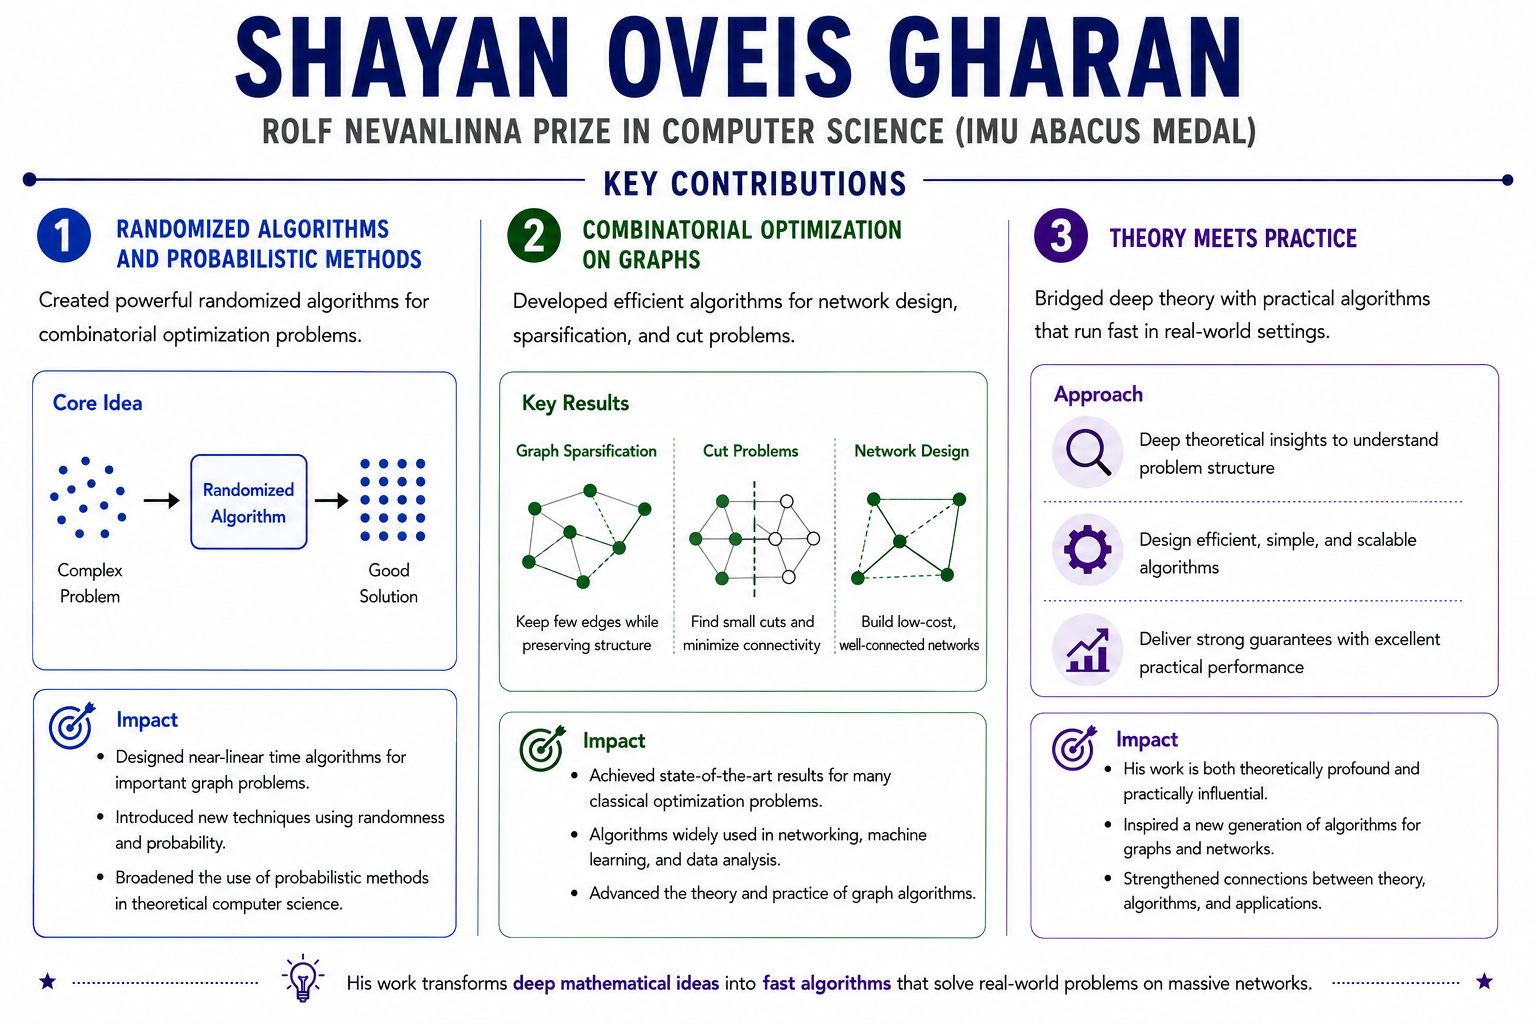
\includegraphics[width=\textwidth]{infographics/abacus12.png}
\end{center}
\index{Oveis Gharan, Shayan}
\booknote{The central habit in this chapter is to encode a combinatorial family as a polynomial, and to read the polynomial's curvature, zeros, and spectra as information about the family.}

\section{An Opening Story: Which Trails Should Stay?}
A small nature reserve has four campsites---north, east, south, and west---joined by five trails forming a square with a diagonal. The rangers must close some trails for maintenance while keeping every campsite reachable from every other. A minimal way to keep the reserve connected is to keep exactly three trails, with none wasted on loops. There are $\binom{5}{3}=10$ ways to choose three of the five trails, but two of those choices form a closed triangle and strand the fourth campsite, leaving $8$ workable choices. Each such choice is a \emph{spanning tree}: three trails that touch all four campsites with no wasted loops.

Now suppose the reserve chooses among the $8$ trees uniformly at random. How likely is each trail to survive? Listing all eight trees answers directly: the diagonal appears in $4$ of them, so it survives with probability $4/8=1/2$; each side trail appears in $5$, so it survives with probability $5/8$. That was easy because the reserve is tiny.

Now add campsites. The complete network on $n$ campsites---every pair directly linked---has $n^{n-2}$ spanning trees: $16$ for $n=4$, about $10^{61}$ (a number with $61$ digits) for $n=40$. The questions ``how many spanning trees?'' and ``how likely is each trail?'' still make sense, but no one will answer them by listing. This is where Oveis Gharan's work begins: the discrete list hides a continuous object---a polynomial---that answers both questions with no listing at all. The 2026 Abacus Medal recognized this habit of reaching for a hidden geometric object when a combinatorial process looks too irregular to control \cite{imu2026}.

\section{The Problem}
Three problems, all phrased as questions a computer must answer without writing out an astronomically large list.

\noindent\textbf{Sampling from a huge family.} Fix a family of combinatorial objects---the spanning trees of a graph, the bases of a matroid, the independent sets of a matroid---and attach a positive weight to every object (for example, the product of weights on its edges). Draw an object at random with probability proportional to its weight. For the four-campsite reserve this is a coin flip among eight trees; for a network of ten thousand sites the family is unimaginably large, yet the answer must come back in seconds.

\noindent\textbf{Approximating the shortest tour.} Given cities with distances obeying the triangle inequality (going directly between two cities is never longer than routing through a third), find the shortest tour that visits every city exactly once. The exact optimum is believed to be computationally hopeless, so the target is a \emph{ratio}: a tour guaranteed to be at most $\alpha$ times the optimum, with $\alpha$ as close to $1$ as possible.

\noindent\textbf{Proving counting inequalities.} Count the independent sets of a matroid by size: $I_k$ independent sets of size $k$. For the uniform matroid on $4$ elements of rank $2$, the counts are $I_0=1$, $I_1=4$, $I_2=6$. Are such sequences always \emph{log-concave}, each term at least the geometric mean of its neighbors, $I_k^2\ge I_{k-1}I_{k+1}$? Mason conjectured a much stronger normalized version in 1978; it stayed open for more than four decades.

All three problems are hard for the same reason: the family is too large to look at, so every argument must summarize the whole family with a smaller object that still remembers the answers.

\section{The World Before}
Before 1976, the travelling salesperson problem had a good heuristic reputation but no provable guarantee. Christofides changed that with an algorithm that is almost ridiculously short to describe, and whose $3/2$ approximation ratio then resisted improvement for roughly forty-five years \cite{christofides76}.

\noindent\textbf{Christofides' architecture.} First build a minimum spanning tree: connect all cities with the cheapest possible set of roads. This costs at most the length of an optimal tour, because deleting one road from any tour leaves a spanning tree. Second, look at the vertices where the tree has an odd number of incident edges---they cannot close into a valid tour yet---and add a minimum-weight perfect matching among exactly those vertices. That matching costs at most half an optimal tour, because an optimal tour, restricted to the odd vertices, splits into two matchings of total length at most the tour. Third, \emph{shortcut}: walk along the tree and the matching and, whenever the walk revisits a city, jump over it. The triangle inequality guarantees that shortcuts never lengthen the tour. Total: $1+\tfrac12=\tfrac32$ times optimal.

\noindent\textbf{Why $3/2$ survived.} The proof is tight: there are instances where the tree alone costs a whole tour and the matching is forced to cost half a tour at the same time. Every improvement attempt used the same division of labor---one argument pays for connectivity, a separate argument pays for parity repair---and each layer kept paying the same bill. After decades it became clear that any real improvement must break the coupling: it must choose a spanning tree whose random choices are correlated with the parity repair that will follow. That requires a distribution over trees with very specific statistical properties, which is exactly what nobody had.

\noindent\textbf{Markov chains, one family at a time.} To sample from a huge family, a standard tool is a \emph{Markov chain}: start with any object, make small random changes (drop an edge, add an edge), and hope the walk quickly forgets where it started. The obstacle is proving \emph{rapid mixing}. Before the work in this chapter, mixing proofs were done family by family with ad hoc tools---conductance arguments that hunt for a bottleneck, couplings that pair two walks and show they meet. Each success looked different, and there was no common certificate a newcomer could reuse.

\noindent\textbf{Log-concavity sat in convex geometry.} Log-concave sequences and functions had a rich life in convex geometry and probability---Brunn--Minkowski theory, Alexandrov--Fenchel inequalities, the geometry of polytopes---but almost nobody connected them to algorithms. Mason's 1978 conjecture about the normalized counts $I_k/\binom nk$ sat exactly at this intersection: clearly combinatorial, provable by no combinatorial tool known then.

\section{The New Idea}
The unifying move is to change the type of the object being studied. A family of discrete objects becomes a single polynomial, and the polynomial's geometry---where it is concave, where its zeros live, what its spectrum is---becomes a certificate that algorithms can consume. Four named ideas form the toolkit.

\subsection{A family becomes a polynomial}
For a graph $G$ with an edge variable $z_e$ per edge, define the \emph{spanning-tree polynomial}
\[
T_G(z)=\sum_{\mathcal{T}\text{ spanning tree}}\;\prod_{e\in\mathcal{T}} z_e,
\]
one monomial per tree. The polynomial is a storage device: the coefficient of a monomial counts the trees containing that set of edges. More importantly, derivatives are exactly the operations an algorithm needs. Setting $z_e=0$ \emph{forbids} edge $e$; differentiating with respect to $z_e$ \emph{forces} it. The ratio $z_e\,\partial_{z_e}\log T_G$, evaluated at $z_e=1$, is the probability that a uniformly random spanning tree contains edge $e$. A combinatorial question about a huge family has become a calculus question about one object.

\subsection{Log-concavity and negative dependence}
A positive polynomial $p$ is \emph{log-concave} on the positive orthant when $\log p$ bends downward in every direction there. The word is geometry, but it can support useful statistical consequences: in the strongly log-concave and matroid settings relevant here, it underlies mixing results and known negative-dependence consequences. Plain log-concavity alone is not equivalent to negative dependence. The stronger hypotheses also survive the operations an algorithm needs: conditioning (take a derivative) and restriction (set variables to zero). A proof that the relevant polynomial is strongly log-concave is therefore a promise that the whole sequence of conditional distributions the algorithm creates will stay well behaved.

\emph{Stable polynomials} are the mechanism that produces log-concavity. A multivariate polynomial is stable when it has no zeros with all variables in the upper half-plane; this is the natural generalization of a one-variable polynomial with all real roots. Real-rootedness was already known to force log-concavity of coefficient sequences, and stability inherits that power in many variables while being closed under exactly the operations---differentiation, specialization, limits---that a proof needs.

\subsection{Spectral independence: a local certificate}
For a distribution on subsets, define the \emph{influence} of one element on another: how much does conditioning on one element being present change the marginal probability of another? A large influence entry is a suspicion of a bottleneck; a large \emph{eigenvalue} of the influence matrix is the real disease, because a matrix can have small entries yet greatly amplify a well-chosen direction. \emph{Spectral independence} requires the largest eigenvalue of every influence matrix---under \emph{every} partial assignment the chain might encounter---to stay bounded. This converts ``prove there is no hidden bottleneck'' into ``bound the eigenvalues of some small matrices,'' and it is exactly the local certificate a fast-mixing proof needs.

\subsection{Entropic rounding: how $3/2$ fell}
The last idea closes the TSP story. Solve a fractional relaxation of the tour problem: a point $x$ in a polytope that mixes connectivity and parity information and costs at most the optimal tour. Then round it to a real tour. The old rounding rules chose edges independently and paid the same parity bill every time. The new rule is \emph{entropic rounding}: choose the distribution over spanning trees with maximum entropy among all distributions whose marginals match $x$, then sample from it. Because the tree polynomial has the required stability and correlation properties, the sampled tree is globally correlated in exactly the way the parity repair needs, and the two bills---connectivity and parity---can no longer both be maximally expensive at once. The result: approximation ratio $3/2-\eps$ for a fixed constant $\eps>10^{-36}$ \cite{karlin-tsp}, the first improvement over Christofides in nearly half a century.

The conceptual shift, in one line: \emph{a family of trees can be a determinant; a distribution can be a polynomial; correlations can be an operator; a mixing proof can be a curvature argument.}

\section{How It Works: Worked Examples}
\subsection{The triangle: three trees, one polynomial}
Take the triangle on vertices $\{1,2,3\}$ with edge weights $a$ (between $1$ and $2$), $b$ (between $2$ and $3$), and $c$ (between $1$ and $3$). Every spanning tree omits exactly one edge, so the spanning-tree polynomial is
\[
T(a,b,c)=ab+ac+bc.
\]
Set $a=b=c=1$. Then $T=3$: the triangle has three spanning trees. Edge $a$ appears in the trees $\{ab,ac\}$, two out of three, so a uniformly random tree contains edge $a$ with probability $2/3$.

Now the polynomial answers the same question by calculus. The derivative
\[
a\,\frac{\partial T}{\partial a}=a(b+c)=1\cdot(1+1)=2
\]
counts, with weight, the trees containing edge $a$; dividing by $T=3$ gives $2/3$. Equivalently, the \emph{logarithmic derivative}
\[
a\,\frac{\partial}{\partial a}\log T=\frac{a(b+c)}{ab+ac+bc}=\frac{2}{3}
\]
is the marginal probability. \emph{A derivative that looks analytic is a probability.}

\subsection{A resistor agrees}
Now treat each edge as a $1$-ohm resistor and compute the \emph{effective resistance} between the endpoints of edge $a$: the resistance of the whole network seen from those two terminals. The route through $b$ and $c$ in series has resistance $1+1=2$ ohms; the direct edge $a$ is a $1$-ohm path in parallel with it, so
\[
R_{\mathrm{eff}}=\frac{1\cdot 2}{1+2}=\frac{2}{3}\ \text{ohms}.
\]
The electrical identity behind random spanning trees (Kirchhoff) says: the probability that an edge belongs to the random tree equals its conductance times the effective resistance between its endpoints. The conductance is $1$, so the probability is $2/3$ again. Two computations that look completely different---counting trees, and reducing resistor networks---deliver the same number. That coincidence is the pattern: \emph{write the partition function, differentiate it, read the derivative as a marginal, and recognize the marginal as a physical quantity.}

The identity is not a special case of equal weights. Try $a=1$, $b=2$, $c=3$: the polynomial gives $T=11$ and probability $a(b+c)/T=5/11$. The series path $b,c$ has resistance $1/2+1/3=5/6$; in parallel with the $1$-ohm edge,
\[
R_{\mathrm{eff}}=\frac{1}{1+6/5}=\frac{5}{11},
\]
and conductance times resistance is $5/11$ again.

\subsection{Mason's conjecture on a small matroid}
A sequence $x_0,x_1,\ldots$ is \emph{log-concave} when $x_k^2\ge x_{k-1}x_{k+1}$ for every $k$: each term is at least the geometric mean of its neighbors. The binomial coefficients $\binom 4k=1,4,6,4,1$ are log-concave, since $4^2=16\ge 1\cdot 6=6$ and $6^2=36\ge 4\cdot 4=16$.

The uniform matroid $U_{2,4}$ keeps every subset of $\{1,2,3,4\}$ of size at most $2$ independent. Its counts are $I_0=1$, $I_1=4$, $I_2=6$---the entries of the binomial row, by design. Mason's conjecture (now a theorem of Anari, Liu, Oveis Gharan, and Vinzant \cite{anari20}) says the \emph{normalized} counts are log-concave:
\[
\left(\frac{I_k}{\binom nk}\right)^2\ge \frac{I_{k-1}}{\binom n{k-1}}\cdot\frac{I_{k+1}}{\binom n{k+1}},
\]
where $n$ is the number of elements of the matroid---for $U_{2,4}$, $n=4$. (Do not normalize by the rank $\binom rk$; the ground-set size $n$ is the right denominator.) Clearing denominators gives the working form
\[
I_k^2\ge I_{k-1}\,I_{k+1}\,\frac{(k+1)(n-k+1)}{k(n-k)}.
\]
Check $k=1$ for $U_{2,4}$:
\[
I_1^2=16,\qquad I_0\,I_2\,\frac{2\cdot 4}{1\cdot 3}=1\cdot 6\cdot\frac{8}{3}=16.
\]
Equality---the uniform matroid is the perfectly balanced case, exactly where the bound is sharp.

The conjecture is meaningful for matroids that are not uniform. Take the graphic matroid of the complete graph $K_4$: its elements are the $6$ edges, and independent sets are forests. The counts are $I_0=1$, $I_1=6$, $I_2=15$ (any two edges), $I_3=16$ (the spanning trees, by Cayley's formula $n^{n-2}=16$), and $I_4=0$. Here $n=6$, and the $k=2$ check reads
\[
I_2^2=225,\qquad I_1\,I_3\,\frac{(3)(5)}{(2)(4)}=6\cdot 16\cdot\frac{15}{8}=180,
\]
and $225\ge 180$ holds. The plain sequence $1,6,15,16$ is log-concave too ($15^2=225\ge 6\cdot 16=96$), but the normalized inequality is strictly stronger, and it is the strong form that powers the algorithms: it is exactly the statement that the independence polynomial is log-concave in the sense needed for fast sampling.

\section{The Mathematics in Brief}
\emph{The spanning-tree polynomial is a determinant.} The matrix-tree theorem: form the weighted Laplacian $L$ with diagonal entries equal to the sum of the edge weights incident to a vertex and off-diagonal entries $-w_{uv}$; delete any one row and column; the determinant is exactly $T_G(z)$. Determinants are more than a computation trick: they give the polynomial a spectral life, including its stability, that pure combinatorics cannot see.

\emph{Log-concavity is a statement about covariance.} For a positive polynomial $p$, the Hessian
\[
\nabla^2\log p=\frac{p\,\nabla^2p-(\nabla p)(\nabla p)^{\mathsf T}}{p^2}
\]
is negative semidefinite exactly when $p$ is log-concave. The first derivatives of $\log p$ are marginal probabilities; the second derivatives, after subtracting products of first derivatives, are conditional covariances. Negative semidefiniteness says these covariances are nonpositive in every direction: negative dependence, uniformly. The ``why'': the numerator is a covariance-like object in disguise, and concavity forbids any direction in which including one element systematically amplifies another.

\emph{Influence matrices.} For a distribution on binary variables and a partial assignment $\tau$, define
\[
\Psi^\tau_{ij}=\PP(X_j=1\mid X_i=1,\tau)-\PP(X_j=1\mid X_i=0,\tau).
\]
Spectral independence requires $\lambda_{\max}(\Psi^\tau)\le C$ for every $\tau$. The eigenvalue, not the entries, is the right measure: the all-ones matrix has every entry $1$ but operator norm $m$, and a chain that must navigate such a collective push needs to know about it.

\emph{Local certificates, global mixing.} The payoff theorem (Asadi, Oveis Gharan, and Saberi \cite{asadi20}; sharpened by Anari, Liu, Oveis Gharan, and Vinzant \cite{anari21}) applies under specific strong log-concavity, spectral-independence, and chain hypotheses; plain log-concavity by itself is not a universal mixing theorem. Under those hypotheses, the relevant local chain mixes rapidly. Sampling then becomes a usable subroutine, and counting rides on it: a telescoping product of partition-function ratios, each factor estimated from samples at a nearby parameter, yields a fully polynomial randomized approximation scheme for counting matroid bases \cite{anari19}.

\emph{The TSP, in two layers.} The subtour-elimination linear program relaxes tours to fractional vectors $x_e$ on edges, costing at most the optimum tour. The rounding layer chooses a distribution over spanning trees whose marginals match $x$ and which has maximum entropy among all such distributions; the relevant stability and strong log-concavity properties of $T_G$ supply the correlation control that keeps the parity-repair bill in check. The layers are inseparable: a relaxation that sees structure is useless without a rounding rule that respects it.

\section{Limits and Modern Views}
The certificate-based picture has boundaries worth knowing before they bite.

\noindent\textbf{Certificates can be hard to verify.} A polynomial may be log-concave or stable, but checking that property computationally is not free, and a theorem about an inaccessible certificate does not by itself produce an algorithm.

\noindent\textbf{Chain steps can be expensive.} Fast mixing is measured in number of steps; the steps themselves must be cheap, and a local move over a huge family may involve a determinant or a linear-system solve per step. The true running time is steps times per-step cost.

\noindent\textbf{Constants hide in guarantees.} The metric TSP improvement is $3/2-\eps$ for a fixed constant $\eps>10^{-36}$ \cite{karlin-tsp}---a genuine theoretical milestone that does not change the number on a real logistics invoice. Approximation theory measures ratios asymptotically; practice measures constants.

\noindent\textbf{Log-concavity fails at phase transitions.} Real systems have regimes---high density, sharp thresholds---where the balanced, negatively dependent world breaks down and bottlenecks reappear. The certificates are true only where their hypotheses hold, and knowing where they fail is part of using them.

The field moved outward from these boundaries. The geometry-of-polynomials program now touches approximate counting, high-dimensional statistical physics, convex geometry, and algebraic combinatorics via Hodge theory; spectral independence has become a standard tool for spin systems and other Gibbs distributions; entropic rounding opened a research line on correlation-aware rounding beyond TSP. Open directions include weaker stability notions that still imply negative dependence, adaptive and nonreversible chain designs, and approximate or learned certificates. The habit of this chapter---encode, then read geometry---survives every one of these changes.

\section{Exercises and Self-Study Guide}
\begin{enumerate}[label=\textbf{E\arabic*.}]
\item List all spanning trees of a path on four vertices and write its weighted spanning-tree polynomial.
\hint{A spanning tree of a four-vertex graph has three edges, and the path has exactly three. There is exactly one tree; the polynomial is a single monomial, and every edge marginal is $1$. Compare with the triangle, where every tree omits one edge.}
\item For the triangle with weights $a=1$, $b=2$, $c=3$, compute the probability that a random weighted tree contains edge $a$, in two ways: from the polynomial $T=ab+ac+bc$, and from the series--parallel effective resistance between the endpoints.
\hint{Both give $5/11$: the series path $b,c$ has resistance $1/2+1/3=5/6$, and in parallel with the $1$-ohm edge the effective resistance is $1/(1+6/5)=5/11$.}
\item Verify Mason's inequality $I_k^2\ge I_{k-1}I_{k+1}(k+1)(n-k+1)/\bigl(k(n-k)\bigr)$ for $U_{2,4}$ at $k=1$ and for the graphic matroid of $K_4$ at $k=2$.
\hint{Use $n=4$ for $U_{2,4}$ and $n=6$ for $K_4$ (the number of edges, not the rank $3$). The counts are $1,4,6$ and $1,6,15,16$; the two checks are equality and $225\ge 180$.}
\item Build the two-state Markov chain with transition matrix $\begin{pmatrix}1-a&a\\b&1-b\end{pmatrix}$. Find its stationary distribution and eigenvalues, and decide when mixing is fast.
\hint{The stationary distribution is proportional to $(b,a)$; the eigenvalues are $1$ and $1-a-b$, so the spectral gap $a+b$ controls the mixing speed.}
\item Give a matrix whose every entry is small but whose operator norm is large.
\hint{The all-ones matrix $J$ has $\norm{J}=m$ while every entry is $1$: the vector $(1,\ldots,1)$ is an eigenvector with eigenvalue $m$. Small entries can still push collectively.}
\item Design a local Markov chain for sampling independent sets of a small graph, and identify a likely bottleneck.
\hint{Use Glauber dynamics: add or delete a vertex while maintaining independence. On a star graph the chain must cross between ``center chosen'' and ``center absent''; thin cuts between such regions control the mixing time.}
\item Compute the total variation distance between the distributions $\mu=(0.9,0.1)$ and $\nu=(0.7,0.3)$ on $\{0,1\}$, and explain what the number means.
\hint{$\norm{\mu-\nu}_{\mathrm{TV}}=\frac12\sum_x\abs{\mu(x)-\nu(x)}=\frac12(0.2+0.2)=0.2$; it is the largest probability gap any event can detect.}
\end{enumerate}

\booknote{A final exercise in judgment: whenever a polynomial makes a combinatorial theorem easy, ask what the polynomial made invisible. It answers questions about marginals, correlations, and counts instantly; it does not show you any single object. Decide, for one of your own problems, whether the algorithm needs a specific object or only its statistics---and if it needs the object, find the way back out.}
\clearpage

\backmatter
\chapter*{Sources and Further Reading}
\addcontentsline{toc}{chapter}{Sources and Further Reading}
\begin{thebibliography}{99}
\bibitem{imu2022} International Mathematical Union, ``Abacus Medal 2022: Mark Braverman,'' official award page, 2022. \url{https://www.mathunion.org/imu-awards/imu-abacus-medal/abacus-medal-2022}.
\bibitem{imu2026} International Mathematical Union, ``Abacus Medal 2026: Shayan Oveis Gharan,'' official award page, 2026. \url{https://www.mathunion.org/imu-awards/imu-abacus-medal/abacus-medal-2026}.
\bibitem{imu-history} International Mathematical Union, ``Rolf Nevanlinna Prize -- Prestigious Award in Mathematical Information Sciences,'' official winners list and history. \url{https://www.mathunion.org/imu-awards/rolf-nevanlinna-prize}.
\bibitem{braverman14} M. Braverman and A. Rao, ``Information equals amortized communication,'' \emph{Proceedings of the 55th IEEE Symposium on Foundations of Computer Science}, 2014.
\bibitem{braverman11} M. Braverman and A. Moitra, ``An information complexity approach to extended formulations,'' \emph{Proceedings of the 43rd ACM Symposium on Theory of Computing}, 2011.
\bibitem{braverman15} M. Braverman, ``Interactive information complexity,'' \emph{Foundations and Trends in Theoretical Computer Science}, 2015.
\bibitem{christofides76} N. Christofides, ``Worst-case analysis of a new heuristic for the travelling salesman problem,'' technical report, Graduate School of Industrial Administration, Carnegie--Mellon University, 1976.
\bibitem{karlin-tsp} A. R. Karlin, N. Klein, and S. Oveis Gharan, ``A (slightly) improved approximation algorithm for metric TSP,'' 2020. arXiv:2007.01409.
\bibitem{asadi20} A. Asadi, S. Oveis Gharan, and A. Saberi, ``Mixing time of the Glauber dynamics for strongly log-concave distributions,'' \emph{Proceedings of the 61st IEEE Symposium on Foundations of Computer Science}, 2020.
\bibitem{anari19} N. Anari, K. Liu, S. Oveis Gharan, and C. Vinzant, ``Log-concave polynomials II: High-dimensional walks and an FPRAS for counting bases of a matroid,'' \emph{Proceedings of the 60th IEEE Symposium on Foundations of Computer Science}, 2019.
\bibitem{anari20} N. Anari, K. Liu, S. Oveis Gharan, and C. Vinzant, ``Log-concave polynomials III: Mason's conjecture for independent sets of matroids,'' \emph{Combinatorica}, 2020.
\bibitem{anari21} N. Anari, K. Liu, S. Oveis Gharan, and C. Vinzant, ``Log-concave polynomials IV: Exchange properties, tight mixing times, and near-linear time sampling of forests,'' \emph{Proceedings of the 54th ACM Symposium on Theory of Computing}, 2022.
\bibitem{spielman12} D. A. Spielman and S.-H. Teng, ``Spectral partitioning works: Planar graphs and finite element meshes,'' \emph{Linear Algebra and its Applications}, 2007.
\bibitem{mcmullen72} P. McMullen, ``The maximum numbers of faces of a convex polytope,'' \emph{Mathematica}, 1970.
\bibitem{tarjan-union} R. E. Tarjan, ``Efficiency of a good but not linear set union algorithm,'' \emph{Journal of the ACM}, 1975.
\bibitem{tarjan-dfs} R. E. Tarjan, ``Depth-first search and linear graph algorithms,'' \emph{SIAM Journal on Computing}, 1972.
\bibitem{valiant-counting} L. G. Valiant, ``The complexity of computing the permanent,'' \emph{Theoretical Computer Science}, 1979.
\bibitem{valiant-learning} L. G. Valiant, ``A theory of the learnable,'' \emph{Communications of the ACM}, 1984.
\bibitem{razborov-monotone} A. A. Razborov, ``Lower bounds on the monotone complexity of some Boolean functions,'' \emph{Soviet Mathematics--Doklady}, 31 (1985), 354--357.
\bibitem{alon-boppana} N. Alon and R. B. Boppana, ``The monotone complexity of Boolean functions,'' \emph{Combinatorica}, 7 (1987), 1--22.
\bibitem{razborov-circuit} A. A. Razborov, ``Unprovability of lower bounds on the circuit size in certain fragments of bounded arithmetic,'' \emph{Izvestiya: Mathematics}, 1995.
\bibitem{wigderson-interactive} S. Goldwasser, S. Micali, and C. Rackoff, ``The knowledge complexity of interactive proof systems,'' \emph{SIAM Journal on Computing}, 1989.
\bibitem{wigderson-zk} O. Goldreich, S. Micali, and A. Wigderson, ``Proofs that yield nothing but their validity or all languages in NP have zero-knowledge proof systems,'' \emph{Journal of the ACM}, 1991.
\bibitem{shor-factoring} P. W. Shor, ``Algorithms for quantum computation: discrete logarithms and factoring,'' \emph{Proceedings of the 35th IEEE Symposium on Foundations of Computer Science}, 1994.
\bibitem{shor-error} P. W. Shor, ``Scheme for reducing decoherence in quantum computer memory,'' \emph{Physical Review A}, 1995.
\bibitem{sudan-list} M. Sudan, ``Decoding of Reed Solomon codes beyond the error-correction bound,'' \emph{Journal of Complexity}, 1997.
\bibitem{sudan-pcp} S. Arora and S. Safra, ``Probabilistic checking of proofs: a new characterization of NP,'' \emph{Journal of the ACM}, 1998.
\bibitem{kleinberg-hits} J. M. Kleinberg, ``Authoritative sources in a hyperlinked environment,'' \emph{Journal of the ACM}, 1999.
\bibitem{kleinberg-smallworld} J. M. Kleinberg, ``The small-world phenomenon: an algorithmic perspective,'' \emph{Proceedings of the 32nd ACM Symposium on Theory of Computing}, 2000.
\bibitem{kleinberg-bursts} J. Kleinberg, ``Bursty and hierarchical structure in streams,'' \emph{Proceedings of the 8th ACM SIGKDD International Conference on Knowledge Discovery and Data Mining}, 2002.
\bibitem{spielman-smoothed} D. A. Spielman and S.-H. Teng, ``Smoothed analysis of algorithms: why the simplex algorithm usually takes polynomial time,'' \emph{Journal of the ACM}, 2004.
\bibitem{spielman-laplacian} D. A. Spielman and S.-H. Teng, ``Nearly-linear time algorithms for graph partitioning, graph sparsification, and solving linear systems,'' \emph{Proceedings of the 36th ACM Symposium on Theory of Computing}, 2004.
\bibitem{spielman-codes} D. A. Spielman, ``Linear-time encodable and decodable error-correcting codes,'' \emph{Proceedings of the 27th ACM Symposium on Theory of Computing}, 1996.
\bibitem{khot-unique} S. Khot, ``On the power of unique 2-prover 1-round games,'' Proceedings of the 34th ACM Symposium on Theory of Computing, 2002.
\bibitem{khot-hardness} S. Khot, G. Kindler, E. Mossel, and R. O'Donnell, ``Optimal inapproximability results for MAX-CUT and other 2-variable CSPs?,'' \emph{SIAM Journal on Computing}, 2007.
\bibitem{goemans-williamson} M. X. Goemans and D. P. Williamson, ``Improved approximation algorithms for maximum cut and satisfiability problems using semidefinite programming,'' \emph{Journal of the ACM}, 42(6), 1115--1145, 1995.
\bibitem{hastad-optimal} J. H\aa stad, ``Some optimal inapproximability results,'' \emph{Journal of the ACM}, 48(4), 798--859, 2001.
\bibitem{raghavendra-csp} P. Raghavendra, ``Optimal algorithms and inapproximability results for every CSP?,'' \emph{Proceedings of the 40th ACM Symposium on Theory of Computing}, 2008.
\bibitem{dkkms-2to2} I. Dinur, S. Khot, G. Kindler, D. Minzer, and M. Safra, ``Towards a proof of the 2-to-1 games conjecture?,'' \emph{Proceedings of the 50th ACM Symposium on Theory of Computing}, 376--389, 2018.
\bibitem{kms-2to2} S. Khot, D. Minzer, and M. Safra, ``Small set expansion in the shortcode graph and the 2-to-2 conjecture,'' arXiv:1804.08662, 2018.
\bibitem{daskalakis-nash} C. Daskalakis, P. W. Goldberg, and C. H. Papadimitriou, ``The complexity of computing a Nash equilibrium,'' \emph{SIAM Journal on Computing}, 2009.
\bibitem{daskalakis-markets} C. Daskalakis, A. Deckelbaum, and C. Tzamos, ``Mechanism design via optimal transport,'' \emph{Proceedings of the 14th ACM Conference on Electronic Commerce}, 2013.
\end{thebibliography}
\printindex
\end{document}
